\documentclass[11pt,a4paper]{report}

% ==============================================================================
% PACKAGES ET CONFIGURATION TYPOGRAPHIQUE
% ==============================================================================
\usepackage[utf8]{inputenc}
\usepackage[T1]{fontenc}
\usepackage[french]{babel}
\usepackage{lmodern}
\usepackage{amsmath,amssymb,amsfonts,amsthm}
\usepackage{graphicx}
\graphicspath{{figures/}{../figures/}}
\usepackage{xcolor}
\usepackage{geometry}
\usepackage{fancyhdr}
\usepackage{lastpage}
\usepackage{booktabs}
\usepackage{tabularx}
\usepackage{array}
\usepackage{listings}
\usepackage{tcolorbox}
\usepackage{tikz}
\usetikzlibrary{shapes.geometric,arrows.meta,positioning,calc,fit}
\usepackage[colorlinks=true,linkcolor=navyblue,citecolor=navyblue,urlcolor=navyblue]{hyperref}

% --- Marges et dimensions ---
\geometry{top=2.5cm, bottom=2.5cm, left=2.3cm, right=2.3cm, headheight=14pt}

% --- Palette de Couleurs ---
\definecolor{navyblue}{RGB}{26, 54, 93}
\definecolor{royalblue}{RGB}{43, 108, 176}
\definecolor{darkcharcoal}{RGB}{45, 55, 72}
\definecolor{lightbg}{RGB}{247, 250, 252}
\definecolor{accentred}{RGB}{155, 44, 44}
\definecolor{tealhpc}{RGB}{44, 122, 123}
\definecolor{goldline}{RGB}{214, 158, 46}

% --- Configuration Listings ---
\lstset{
    language=Python,
    basicstyle=\ttfamily\footnotesize\color{darkcharcoal},
    keywordstyle=\bfseries\color{royalblue},
    stringstyle=\color{accentred},
    commentstyle=\itshape\color{gray},
    numbers=left,
    numberstyle=\tiny\color{gray},
    stepnumber=1,
    numbersep=8pt,
    backgroundcolor=\color{lightbg},
    showspaces=false,
    showstringspaces=false,
    showtabs=false,
    frame=single,
    rulecolor=\color{gray!30},
    tabsize=4,
    captionpos=b,
    breaklines=true,
    breakatwhitespace=false,
    xleftmargin=15pt,
    framexleftmargin=15pt,
    inputencoding=utf8,
    extendedchars=true,
    literate=
        {é}{{\'e}}1 {è}{{\`e}}1 {à}{{\`a}}1 {ê}{{\^e}}1 {ë}{{\"e}}1
        {î}{{\^i}}1 {ï}{{\"i}}1 {ô}{{\^o}}1 {û}{{\^u}}1 {ù}{{\`u}}1
        {ç}{{\c{c}}}1 {É}{{\'E}}1 {È}{{\`E}}1 {À}{{\`A}}1 {œ}{{\oe}}1
        {µ}{{$\mu$}}1 {°}{{$^\circ$}}1 {—}{{---}}1 {’}{{'}}1 {…}{{\dots}}1
}

% --- Théorèmes et Propositions ---
\theoremstyle{plain}
\newtheorem{theorem}{Théorème}[chapter]
\newtheorem{proposition}{Proposition}[chapter]
\newtheorem{lemma}{Lemme}[chapter]
\theoremstyle{definition}
\newtheorem{definition}{Définition}[chapter]
\theoremstyle{remark}
\newtheorem{remark}{Remarque}[chapter]

% --- En-têtes et Pieds de Page ---
\pagestyle{fancy}
\fancyhf{}
\fancyhead[L]{\small\itshape Implémentation du modèle d'infection par le VIH-SIDA -- BLAS et LAPACK}
\fancyhead[R]{\small\bfseries\color{navyblue} Groupe 5}
\fancyfoot[L]{\small\color{gray} ENSGMM1 -- UNSTIM (Abomey)}
\fancyfoot[C]{\small\color{gray} UE : Outils de calcul scientifique}
\fancyfoot[R]{\small\bfseries\color{navyblue} Page \thepage\ sur \pageref{LastPage}}
\renewcommand{\headrulewidth}{0.5pt}
\renewcommand{\footrulewidth}{0.5pt}

\fancypagestyle{plain}{
    \fancyhf{}
    \fancyfoot[L]{\small\color{gray} ENSGMM1 -- UNSTIM (Abomey)}
    \fancyfoot[C]{\small\color{gray} UE : Outils de calcul scientifique}
    \fancyfoot[R]{\small\bfseries\color{navyblue} Page \thepage\ sur \pageref{LastPage}}
    \renewcommand{\headrulewidth}{0pt}
    \renewcommand{\footrulewidth}{0.5pt}
}

% ==============================================================================
% DÉBUT DU DOCUMENT
% ==============================================================================
\begin{document}

% ------------------------------------------------------------------------------
% PAGE DE GARDE OFFICIELLE
% ------------------------------------------------------------------------------
\begin{titlepage}
    \begin{tikzpicture}[remember picture, overlay]
        \draw[line width=1.5pt, color=navyblue] 
            ($(current page.north west) + (1.2cm,-1.2cm)$) rectangle 
            ($(current page.south east) + (-1.2cm,1.2cm)$);
        \draw[line width=0.6pt, color=goldline] 
            ($(current page.north west) + (1.35cm,-1.35cm)$) rectangle 
            ($(current page.south east) + (-1.35cm,1.35cm)$);

        % Logos positionnés dans les coins supérieurs intérieurs
        \node[anchor=north west, inner sep=0pt] at ($(current page.north west) + (1.6cm,-1.6cm)$) {
            
\includegraphics[height=2.3cm]{figures/logo_unstim.png}
        };
        \node[anchor=north east, inner sep=0pt] at ($(current page.north east) + (-1.6cm,-1.6cm)$) {
            
\includegraphics[height=2.3cm]{figures/logo_ensgmm.png}
        };
    \end{tikzpicture}

    \centering
    \vspace*{0.5cm}

    {\fontsize{11}{14}\selectfont \textsc{\textbf{République du Bénin}}}\\[0.15cm]
    {\fontsize{10}{13}\selectfont \textbf{Ministère de l'Enseignement Supérieur et de la Recherche Scientifique}}\\[0.25cm]
    {\fontsize{12}{15}\selectfont \textsc{\textbf{Université Nationale des Sciences, Technologies,}}}\\[0.1cm]
    {\fontsize{12}{15}\selectfont \textsc{\textbf{Ingénierie et Mathématiques d'Abomey (UNSTIM)}}}\\[0.25cm]
    {\fontsize{12.5}{15.5}\selectfont \textcolor{navyblue}{\textbf{École Nationale des Génies Mathématiques et Modélisation (ENSGMM)}}}

    \vspace{0.4cm}
    \textcolor{goldline}{\rule{0.75\textwidth}{1.2pt}}
    \vspace{0.5cm}

    \begin{tcolorbox}[
        colback=navyblue!4!white,
        colframe=navyblue,
        arc=4pt,
        boxrule=1.2pt,
        width=0.96\textwidth,
        halign=center
    ]
        \vspace{0.25cm}
        {\fontsize{19}{23}\selectfont \textbf{\textcolor{navyblue}{Implémentation du modèle d'infection}}}\\[0.2cm]
        {\fontsize{22}{26}\selectfont \textbf{\textcolor{accentred}{par le VIH-SIDA}}}\\[0.35cm]
        {\fontsize{11}{14}\selectfont \textbf{\textit{Modèles intra-hôte et de population : analyse mathématique,}}}\\[0.1cm]
        {\fontsize{11}{14}\selectfont \textbf{\textit{stabilité et résolution numérique avec BLAS, LAPACK et Intel MKL en Python}}}
        \vspace{0.25cm}
    \end{tcolorbox}

    \vspace{0.55cm}

    {\fontsize{12.5}{15}\selectfont \textbf{\textcolor{navyblue}{\textsc{Équipe de projet -- Groupe 5}}}}\\[0.35cm]
    {\large \textbf{ADOGOUN}} Déo Gracias Mahugnon\\[0.15cm]
    {\large \textbf{BIAHOU}} Ahossou J. Marie-Clémenceau\\[0.15cm]
    {\large \textbf{SYLLA IMOROU}} Izou Dine

    \vspace{0.4cm}

    \begin{tcolorbox}[
        colback=lightbg,
        colframe=royalblue!40,
        boxrule=0.6pt,
        arc=3pt,
        width=0.92\textwidth,
        halign=center
    ]
        \footnotesize
        \textbf{\textcolor{navyblue}{Dépôt GitHub officiel (Code, Simulations \& Reproductibilité) :}}\\[0.08cm]
        \url{https://github.com/JuniorB573/OCS-Groupe5}
    \end{tcolorbox}

    \vfill

    \begin{tcolorbox}[
        colback=lightbg,
        colframe=gray!40,
        boxrule=0.5pt,
        arc=3pt,
        width=0.92\textwidth,
        halign=center
    ]
        \centering
        \small
        \textbf{Promotion :} ENSGMM1 \quad $\bullet$ \quad \textbf{UE :} Outils de calcul scientifique\\[0.1cm]
        \textbf{Année académique :} 2026--2027\\[0.15cm]
        \textbf{Sous la direction de :} \textbf{\textcolor{navyblue}{Dr. Carlos AGOSSOU}}
    \end{tcolorbox}
    \vspace*{-0.2cm}
\end{titlepage}

% ------------------------------------------------------------------------------
% TABLE DES MATIÈRES
% ------------------------------------------------------------------------------
\newpage
\pagenumbering{roman}
\tableofcontents
\newpage
\pagenumbering{arabic}

% ------------------------------------------------------------------------------
% INTRODUCTION
% ------------------------------------------------------------------------------
\chapter*{Introduction}
\addcontentsline{toc}{chapter}{Introduction}

\begin{tcolorbox}[colback=navyblue!90!black,colframe=navyblue!90!black,arc=2pt,coltext=white,boxrule=0pt]
\textbf{\large Résumé Exécutif \& Comprendre le Projet en 1 Minute}
\end{tcolorbox}
\vspace{-0.3cm}
\begin{tcolorbox}[colback=blue!5!white,colframe=navyblue!80!black,arc=2pt,boxrule=0.8pt]
Ce rapport présente une étude complète de la dynamique de l'infection par le virus de l'immunodéficience humaine (VIH), articulée à deux échelles fondamentales : l'échelle du patient (modèle intra-hôte $T, I, V$) et l'échelle d'une communauté (modèle épidémiologique de population $S, I_1, I_2$).\\
\textbf{L'enjeu informatique et scientifique :} Les équations différentielles sous-jacentes sont non-linéaires et fortement raides (\textit{stiff}). Les résoudre sur des horizons de temps longs sans instabilité exige des schémas implicites et des résolutions matricielles directes. Nous montrons comment la pile logicielle formée par \textbf{BLAS}, \textbf{LAPACK} (routines \texttt{DGESV}, \texttt{DGEEV}, \texttt{DGEEQU}, \texttt{DGESDD}) et \textbf{Intel MKL} permet d'atteindre des accélérations de calcul spectaculaires (facteur $\times 200$ à $\times 900$) face aux implémentations naïves.
\end{tcolorbox}

\vspace{0.4cm}
\noindent\textbf{Contexte.} Le calcul scientifique moderne repose sur quelques briques logicielles d'algèbre linéaire dense, BLAS et LAPACK, dont des implémentations très optimisées existent (Intel MKL, OpenBLAS, BLIS). Presque tous les environnements de calcul scientifique (NumPy, SciPy, MATLAB, R, Julia) les utilisent en arrière-plan.

\vspace{0.3cm}
\noindent\textbf{Objectifs de ce rapport.}
\begin{enumerate}
    \item Présenter l'architecture des bibliothèques BLAS, LAPACK et Intel MKL ;
    \item Montrer comment les configurer et les appeler directement depuis Python ;
    \item Les mettre en pratique sur un cas d'étude médical à deux échelles : celle du patient (modèle intra-hôte de Nowak et May / Perelson) et celle de la population (modèle épidémiologique à deux stades avec mortalités) ;
    \item Mesurer leurs performances numériques et leur scalabilité multi-threads face à des implémentations ordinaires.
\end{enumerate}

\vspace{0.3cm}
\noindent\textbf{Organisation.} Les chapitres 1 à 3 détaillent les bibliothèques logicielles (BLAS, LAPACK, puis Intel MKL). Le chapitre 4 présente l'installation et l'appel depuis Python. Le chapitre 5 expose le contexte biologique. Les chapitres 6 à 9 traitent le modèle intra-hôte ($T, I, V$). Le chapitre 10 étudie le modèle de population ($S, I_1, I_2$). Le chapitre 11 présente les résultats des benchmarks d'accélération. Les codes sources complets sont reproduits en annexes.

% ------------------------------------------------------------------------------
% CHAPITRE 1 : BLAS (ORDRE OBLIGATOIRE : 1. BLAS)
% ------------------------------------------------------------------------------
\chapter{BLAS (Basic Linear Algebra Subprograms)}

\section{Origine et philosophie de conception}
Créée à la fin des années 1970 par Lawson et al., BLAS est une spécification d'opérations élémentaires. Sa standardisation garantit la portabilité : l'application appelle la même routine (\texttt{DGEMM}), et le constructeur fournit le binaire optimisé pour son matériel.

\section{Les trois niveaux de BLAS et l'intensité arithmétique}
Le tableau \ref{tab:blas_levels} récapitule la taxonomie des trois niveaux.

\begin{table}[htbp]
\centering
\caption{Les trois niveaux de BLAS et leur intensité arithmétique.}
\label{tab:blas_levels}
\small
\begin{tabularx}{\textwidth}{clcccX}
\toprule
\textbf{Niveau} & \textbf{Opérations} & \textbf{Données} & \textbf{Calculs} & \textbf{Intensité} & \textbf{Exemples phares} \\
\midrule
1 & Vecteur-Vecteur & $\mathcal{O}(n)$ & $\mathcal{O}(n)$ & $\mathcal{O}(1)$ (Faible) & \texttt{DAXPY} ($y \leftarrow \alpha x + y$), \texttt{DDOT}, \texttt{DNRM2} \\
2 & Matrice-Vecteur & $\mathcal{O}(n^2)$ & $\mathcal{O}(n^2)$ & $\mathcal{O}(1)$ (Faible) & \texttt{DGEMV} ($y \leftarrow \alpha Ax + \beta y$), \texttt{DGER}, \texttt{DTRSV} \\
3 & Matrice-Matrice & $\mathcal{O}(n^2)$ & $\mathcal{O}(n^3)$ & $\mathcal{O}(n)$ (Élevée) & \texttt{DGEMM} ($C \leftarrow \alpha AB + \beta C$), \texttt{DSYRK}, \texttt{DTRSM} \\
\bottomrule
\end{tabularx}
\end{table}

\noindent\textbf{Le secret de BLAS 3 : le cache tiling.} Dans les niveaux 1 et 2, pour chaque nombre lu en mémoire, le CPU n'exécute qu'une seule opération : le bus mémoire sature immédiatement (\textit{Memory-Bound}). Dans le niveau 3, pour $n^2$ nombres chargés, on réalise $n^3$ opérations. En découpant les matrices en sous-blocs de taille $B \times B$ calibrés pour tenir dans le cache L1, chaque élément est réutilisé $B$ fois sur place, atteignant la vitesse de crête du processeur (\textit{Compute-Bound}).

\section{Conventions de nommage universelles}
La signature suit la structure \texttt{[Type][Matrice][Opération]} :
\begin{itemize}
    \item \textbf{Type :} \texttt{S} (réel 32 bits), \texttt{D} (réel 64 bits double), \texttt{C} (complexe simple), \texttt{Z} (complexe double).
    \item \textbf{Structure :} \texttt{GE} (générale), \texttt{SY} (symétrique), \texttt{TR} (triangulaire), \texttt{GB} (bande).
    \item \textbf{Opération :} \texttt{MM} (produit matrice-matrice), \texttt{MV} (matrice-vecteur), \texttt{RK} (mise à jour de rang $k$).
\end{itemize}

% ------------------------------------------------------------------------------
% CHAPITRE 2 : LAPACK (ORDRE OBLIGATOIRE : 2. LAPACK)
% ------------------------------------------------------------------------------
\chapter{LAPACK (Linear Algebra PACKage)}

\section{Présentation et Algorithmes par Blocs}
Apparue au début des années 1990 pour succéder à LINPACK et EISPACK, LAPACK réorganise les algorithmes d'algèbre linéaire avancée en \textbf{algorithmes par blocs}. Au lieu de factoriser colonne par colonne, LAPACK factorise un panneau vertical puis met à jour tout le reste de la matrice d'un coup avec \texttt{DGEMM} (BLAS 3), garantissant une efficacité maximale.

\section{Fonctionnalités et routines pilotes}
\begin{table}[htbp]
\centering
\caption{Principales fonctionnalités de LAPACK.}
\label{tab:lapack_routines}
\small
\begin{tabularx}{\textwidth}{llXl}
\toprule
\textbf{Problème mathématique} & \textbf{Routine Pilote} & \textbf{Algorithme sous-jacent} & \textbf{Complexité} \\
\midrule
Système général $Ax = b$ & \texttt{DGESV} & Factorisation LU avec pivotage partiel ($PA = LU$) & $\frac{2}{3}n^3$ \\
Système symétrique défini positif & \texttt{DPOSV} & Factorisation de Cholesky ($A = LL^T$) & $\frac{1}{3}n^3$ \\
Moindres carrés $\min \|Ax - b\|_2$ & \texttt{DGELS} & Décomposition orthogonale QR & $\frac{4}{3}n^3$ \\
Valeurs propres symétriques & \texttt{DSYEV} & Tridiagonalisation + Divide \& Conquer & $\mathcal{O}(n^3)$ \\
Valeurs propres générales & \texttt{DGEEV} & Réduction de Hessenberg + QR décalé & $\mathcal{O}(n^3)$ \\
Décomposition SVD ($A = U\Sigma V^T$) & \texttt{DGESVD} & Bidiagonalisation QR & $\mathcal{O}(n^3)$ \\
Équilibrage de matrice & \texttt{DGEEQU} & Équilibrage de lignes et colonnes & $\mathcal{O}(n^2)$ \\
Estimation conditionnement & \texttt{DGECON} & Estimation de $\|A^{-1}\|_1$ sans inversion & $\mathcal{O}(n^2)$ \\
\bottomrule
\end{tabularx}
\end{table}

\section{Schéma vectoriel de la pile logicielle}
La figure \ref{fig:software_stack} illustre l'empilement logiciel menant de l'application scientifique jusqu'au matériel processeur.

\begin{figure}[htbp]
\centering
\begin{tikzpicture}[
    box/.style={draw=navyblue, fill=blue!5!white, thick, rounded corners=3pt, minimum width=11cm, minimum height=0.75cm, align=center, font=\small\bfseries},
    arrow/.style={-{Stealth[length=2.5mm]}, thick, navyblue}
]
    \node[box] (app) at (0, 4) {Application Python (Modèles VIH, Intégrateurs EDO, Newton)};
    \node[box] (scipy) at (0, 3) {NumPy / SciPy (\texttt{scipy.linalg.lapack}, \texttt{scipy.linalg.blas})};
    \node[box] (lapack) at (0, 2) {LAPACK : \texttt{DGESV}, \texttt{DGETRF}, \texttt{DGEEV}, \texttt{DGEEQU}, \texttt{DGESDD}};
    \node[box] (blas) at (0, 1) {BLAS : \texttt{DGEMM}, \texttt{DGEMV}, \texttt{DAXPY}, \texttt{DDOT}, \texttt{DSYRK}};
    \node[box, fill=tealhpc!10!white, draw=tealhpc] (mkl) at (0, 0) {Micro-noyaux optimisés : Intel MKL (AVX-512, OpenMP) ou OpenBLAS};

    \draw[arrow] (app) -- (scipy);
    \draw[arrow] (scipy) -- (lapack);
    \draw[arrow] (lapack) -- (blas);
    \draw[arrow] (blas) -- (mkl);
\end{tikzpicture}
\caption{Pile logicielle : de l'application scientifique aux noyaux assembleurs optimisés.}
\label{fig:software_stack}
\end{figure}

% ------------------------------------------------------------------------------
% CHAPITRE 3 : INTEL ONEMKL (ORDRE OBLIGATOIRE : 3. INTEL ONEMKL)
% ------------------------------------------------------------------------------
\chapter{Présentation d'Intel MKL (oneMKL)}

\section{Qu'est-ce qu'Intel MKL ?}
Intel oneAPI Math Kernel Library (\textbf{oneMKL}, anciennement Intel MKL) est une bibliothèque industrielle de routines mathématiques ultra-optimisées pour le calcul scientifique et l'ingénierie sur architectures x86-64. Elle tire le meilleur parti des jeux d'instructions vectorielles des microprocesseurs (SSE, AVX2, AVX-512, Intel AMX) et du parallélisme multi-c\oe urs via OpenMP et Intel TBB. Au démarrage, son \textit{CPU Dispatcher} détecte dynamiquement le modèle exact du processeur hôte pour router l'exécution vers les micro-noyaux assembleurs les plus rapides.

\section{Domaines couverts}
\begin{itemize}
    \item \textbf{Algèbre linéaire dense :} BLAS (niveaux 1, 2, 3), LAPACK et ScaLAPACK (calcul parallèle distribué sur grappes MPI).
    \item \textbf{Algèbre linéaire creuse :} Sparse BLAS et solveur direct multithread PARDISO.
    \item \textbf{Transformées de Fourier rapides (FFT) :} Interface compatible FFTW multidimensionnelle.
    \item \textbf{Mathématiques vectorielles (VML) :} Fonctions transcendantes (\texttt{vdExp}, \texttt{vdLn}, \texttt{vdSin}, \texttt{vdInvSqrt}) calculées sur des vecteurs entiers en un cycle SIMD.
    \item \textbf{Statistiques et nombres aléatoires (VSL) :} Générateurs pseudo-aléatoires haute performance.
\end{itemize}

\section{Avantages et alternatives du marché}
Intel MKL offre les meilleures performances crêtes sur processeurs Intel et compatibles AMD. Le tableau \ref{tab:mkl_alternatives} synthétise le paysage des bibliothèques concurrentes.

\begin{table}[htbp]
\centering
\caption{Principales alternatives à Intel MKL.}
\label{tab:mkl_alternatives}
\small
\begin{tabularx}{\textwidth}{llX}
\toprule
\textbf{Bibliothèque} & \textbf{Nature / Licence} & \textbf{Spécificités techniques} \\
\midrule
\textbf{OpenBLAS} & Libre (BSD) & Dérivée de GotoBLAS2 ; livrée par défaut avec NumPy/SciPy sur Linux/macOS. \\
\textbf{BLIS} & Libre (BSD) & Cadre modulaire développé à l'UT Austin avec micro-noyaux portables. \\
\textbf{ATLAS} & Libre & Optimisation automatique hors-ligne lors de l'étape de compilation. \\
\textbf{Netlib} & Libre (Référence) & Code Fortran de référence étalon, sans vectorisation matérielle. \\
\textbf{Intel oneMKL} & Propriétaire gratuit & Code assembleur spécifique, vectorisation AVX-512 et threading OpenMP. \\
\bottomrule
\end{tabularx}
\end{table}

% ------------------------------------------------------------------------------
% CHAPITRE 4 : INSTALLATION, CONFIGURATION ET UTILISATION
% ------------------------------------------------------------------------------
\chapter{Installation, Configuration et Utilisation}

\section{Configuration sous Python et vérification du backend}
NumPy et SciPy peuvent être liés soit à OpenBLAS (via les roues standard pip), soit à Intel MKL (via la distribution conda). La vérification dynamique de la bibliothèque active s'effectue simplement :

\begin{lstlisting}
import numpy as np
from threadpoolctl import threadpool_info

print(np.show_config())        # Configuration BLAS/LAPACK de NumPy
print(threadpool_info())       # Bibliothèque liée, version et nombre de threads
\end{lstlisting}

\section{Appel direct de LAPACK depuis Python}
SciPy offre une interface de bas niveau zéro-copie vers les routines Fortran de LAPACK :

\begin{lstlisting}
from scipy.linalg import lapack
import numpy as np

A = np.asfortranarray([[4.0, 1.0], [2.0, 3.0]])
b = np.array([1.0, 2.0])

# Résolution LU directe Ax = b
lu, piv, x, info = lapack.dgesv(A, b)
assert info == 0, "Échec de factorisation"

# Calcul des valeurs propres (parties réelles et imaginaires)
wr, wi, vl, vr, info = lapack.dgeev(A)
valeurs_propres = wr + 1j * wi
\end{lstlisting}

% ------------------------------------------------------------------------------
% CHAPITRE 5 : LE VIH-SIDA : CONTEXTE BIOLOGIQUE ET ÉCHELLES
% ------------------------------------------------------------------------------
\chapter{Le VIH-SIDA : Contexte Biologique et Échelles}

\section{Physiopathologie de l'infection}
Le Virus de l'Immunodéficience Humaine (VIH) cible spécifiquement les lymphocytes auxiliaires T CD4+, pivot de la coordination immunitaire. Un virion libre pénètre dans une cellule T saine, rétrotranscrit son ARN en ADN proviral et détourne la cellule pour produire de nouveaux virions avant sa mort par apoptose ou cytotoxicité. Chez un patient non traité, l'infection évolue selon trois phases :
\begin{enumerate}
    \item \textbf{Phase aiguë (semaines) :} Pic de charge virale et effondrement temporaire des CD4+ ;
    \item \textbf{Phase chronique (années) :} Équilibre dynamique stationnaire (\textit{set point}) ;
    \item \textbf{Stade SIDA :} Chute irréversible des CD4+ en dessous du seuil critique de 200 cellules/$\mu$L, ouvrant la voie aux infections opportunistes mortelles.
\end{enumerate}

\section{Nécessité de deux échelles de modélisation}
\begin{itemize}
    \item \textbf{Échelle intra-hôte (dans le patient) :} Modèle ($T, I, V$) en jours. Analyse de la charge virale, de la résilience et de l'efficacité thérapeutique $\eta$.
    \item \textbf{Échelle de population (épidémiologique) :} Modèle ($S, I_1, I_2$) en années. Analyse de la prévalence et des interventions de santé publique.
\end{itemize}

% ------------------------------------------------------------------------------
% CHAPITRE 6 : LE MODÈLE INTRA-HÔTE : FORMULATION ET ANALYSE
% ------------------------------------------------------------------------------
\chapter{Le Modèle Intra-Hôte : Formulation et Analyse}

\section{Formulation mathématique}
Le modèle de Nowak-May-Perelson avec traitement antirétroviral d'efficacité $\eta \in [0, 1]$ s'écrit :
\begin{equation}
\label{eq:intra_host}
\begin{cases}
\dfrac{dT}{dt} = s - dT - (1 - \eta)\beta T V \\[0.2cm]
\dfrac{dI}{dt} = (1 - \eta)\beta T V - \delta I \\[0.2cm]
\dfrac{dV}{dt} = p I - c V
\end{cases}
\end{equation}

\begin{figure}[htbp]
\centering
\begin{tikzpicture}[
    compartment/.style={draw=navyblue, fill=blue!5!white, thick, minimum width=2.4cm, minimum height=1.1cm, align=center, font=\small\bfseries},
    arrow/.style={-{Stealth[length=2.5mm]}, thick, navyblue}
]
    \node[compartment] (T) at (0, 0) {T\\CD4+ saines};
    \node[compartment] (I) at (4.2, 0) {I\\Cellules infectées};
    \node[compartment] (V) at (8.4, 0) {V\\Virions libres};

    \draw[arrow] (-1.8, 0) -- node[above, font=\small] {$s$} (T);
    \draw[arrow] (T) -- node[right, font=\small] {$dT$} (0, -1.5);
    \draw[arrow] (T) -- node[above, font=\small] {$(1 - \eta)\beta T V$} (I);
    \draw[arrow] (I) -- node[right, font=\small] {$\delta I$} (4.2, -1.5);
    \draw[arrow] (I) -- node[above, font=\small] {$p I$} (V);
    \draw[arrow] (V) -- node[right, font=\small] {$c V$} (8.4, -1.5);
\end{tikzpicture}
\caption{Schéma de transfert compartimental du modèle intra-hôte.}
\label{fig:transfer_intra}
\end{figure}

\begin{table}[htbp]
\centering
\caption{Paramètres biomédicaux du modèle intra-hôte.}
\label{tab:params_intra}
\small
\begin{tabularx}{\textwidth}{llccX}
\toprule
\textbf{Symbole} & \textbf{Signification} & \textbf{Valeur} & \textbf{Unité} & \textbf{Source de calibration} \\
\midrule
$s$ & Production de CD4+ saines & 10 & cellules/$\mu$L/jour & Hypothèse physiologique \\
$d$ & Mortalité naturelle des CD4+ & 0,01 & jour$^{-1}$ & Perelson \& Nelson ($T_0 = s/d = 1000$) \\
$\beta$ & Infectivité virale & $4{,}6 \times 10^{-5}$ & $\mu$L/virion/jour & Calibré pour $\mathcal{R}_0 = 4$ \\
$\delta$ & Mortalité des cellules infectées & 0,50 & jour$^{-1}$ & Demi-vie virale $\approx 1{,}4$ jour \\
$p$ & Production de virions par cellule & 1000 & virions/cellule/jour & Nowak \& May \\
$c$ & Clairance des virions libres & 23 & jour$^{-1}$ & Demi-vie plasmatique $\approx 5{,}5$ h \\
$\eta$ & Efficacité thérapeutique ARV & 0 à 1 & -- & Paramètre de contrôle clinique \\
\bottomrule
\end{tabularx}
\end{table}

\section{Positivité, Bornitude et Nombre de Reproduction $\mathcal{R}_0$}
\begin{proposition}
Pour toute condition initiale positive, les solutions de (\ref{eq:intra_host}) existent pour tout $t \ge 0$, restent strictement positives, et vérifient $\limsup_{t \to \infty} T(t) \le s/d$.
\end{proposition}

\noindent\textbf{Calcul du $\mathcal{R}_0$ par la Matrice de Prochaine Génération (NGM) :} Posons $b = (1 - \eta)\beta$. Pour le sous-système infecté $(I, V)^T$, la matrice de transmission $F$ et la matrice de transition $V_m$ s'écrivent :
\[
F = \begin{pmatrix} 0 & b T_0 \\ 0 & 0 \end{pmatrix}, \quad V_m = \begin{pmatrix} \delta & 0 \\ -p & c \end{pmatrix} \implies V_m^{-1} = \begin{pmatrix} 1/\delta & 0 \\ p/(\delta c) & 1/c \end{pmatrix}
\]
Le rayon spectral de $F V_m^{-1}$ donne le nombre de reproduction de base :
\begin{equation}
\label{eq:r0_intra}
\mathcal{R}_0(\eta) = \frac{(1 - \eta)\beta p T_0}{\delta c} = (1 - \eta)\mathcal{R}_0(0), \quad \text{avec } \eta_c = 1 - \frac{1}{\mathcal{R}_0(0)} = 75{,}0\,\%
\end{equation}

\section{Stabilité Locale et Globale}
\begin{theorem}[Stabilité du DFE]
L'équilibre sans infection $E_0 = (T_0, 0, 0)$ est globalement asymptotiquement stable (GAS) si $\mathcal{R}_0 \le 1$, et instable si $\mathcal{R}_0 > 1$.
\end{theorem}

\begin{proof}
Considérons la fonction de Lyapunov $L = I + \frac{\delta}{p}V \ge 0$. Sa dérivée le long des trajectoires vaut $\dot{L} = (b T - \frac{\delta c}{p})V$. Comme $T \le T_0$, on a $\dot{L} \le \frac{\delta c}{p}(\mathcal{R}_0 - 1)V \le 0$ lorsque $\mathcal{R}_0 \le 1$. Le principe d'invariance de LaSalle conclut à la stabilité globale du DFE.
\end{proof}

\begin{theorem}[Stabilité de l'Équilibre Endémique EE]
Pour $\mathcal{R}_0 > 1$, l'équilibre endémique $E^* = (T^*, I^*, V^*)$ existe, est unique, et est globalement asymptotiquement stable dans le domaine positif avec :
\[
T^* = \frac{T_0}{\mathcal{R}_0}, \quad I^* = \frac{s}{\delta}\left(1 - \frac{1}{\mathcal{R}_0}\right), \quad V^* = \frac{p}{c} I^* = \frac{p s}{c \delta}\left(1 - \frac{1}{\mathcal{R}_0}\right)
\]
\end{theorem}

% ------------------------------------------------------------------------------
% CHAPITRE 7 : MÉTHODES NUMÉRIQUES ET LAPACK
% ------------------------------------------------------------------------------
\chapter{Méthodes Numériques et LAPACK}

\section{Systèmes linéaires, erreur directe et conditionnement}
La résolution de $Ax = b$ via \texttt{DGETRF} et \texttt{DGETRS} (regroupés dans \texttt{DGESV}) réalise une élimination de Gauss rétrograde-stable. La figure \ref{fig:hilbert} illustre l'évaluation du conditionnement sur des matrices de Hilbert : le résidu reste au niveau de la précision machine ($\approx 10^{-16}$), tandis que l'erreur directe croît proportionnellement à $\kappa_1(A)\,\varepsilon_{\text{mach}}$.

\begin{figure}[htbp]
\centering
\begin{minipage}[t]{0.48\textwidth}
    \centering
    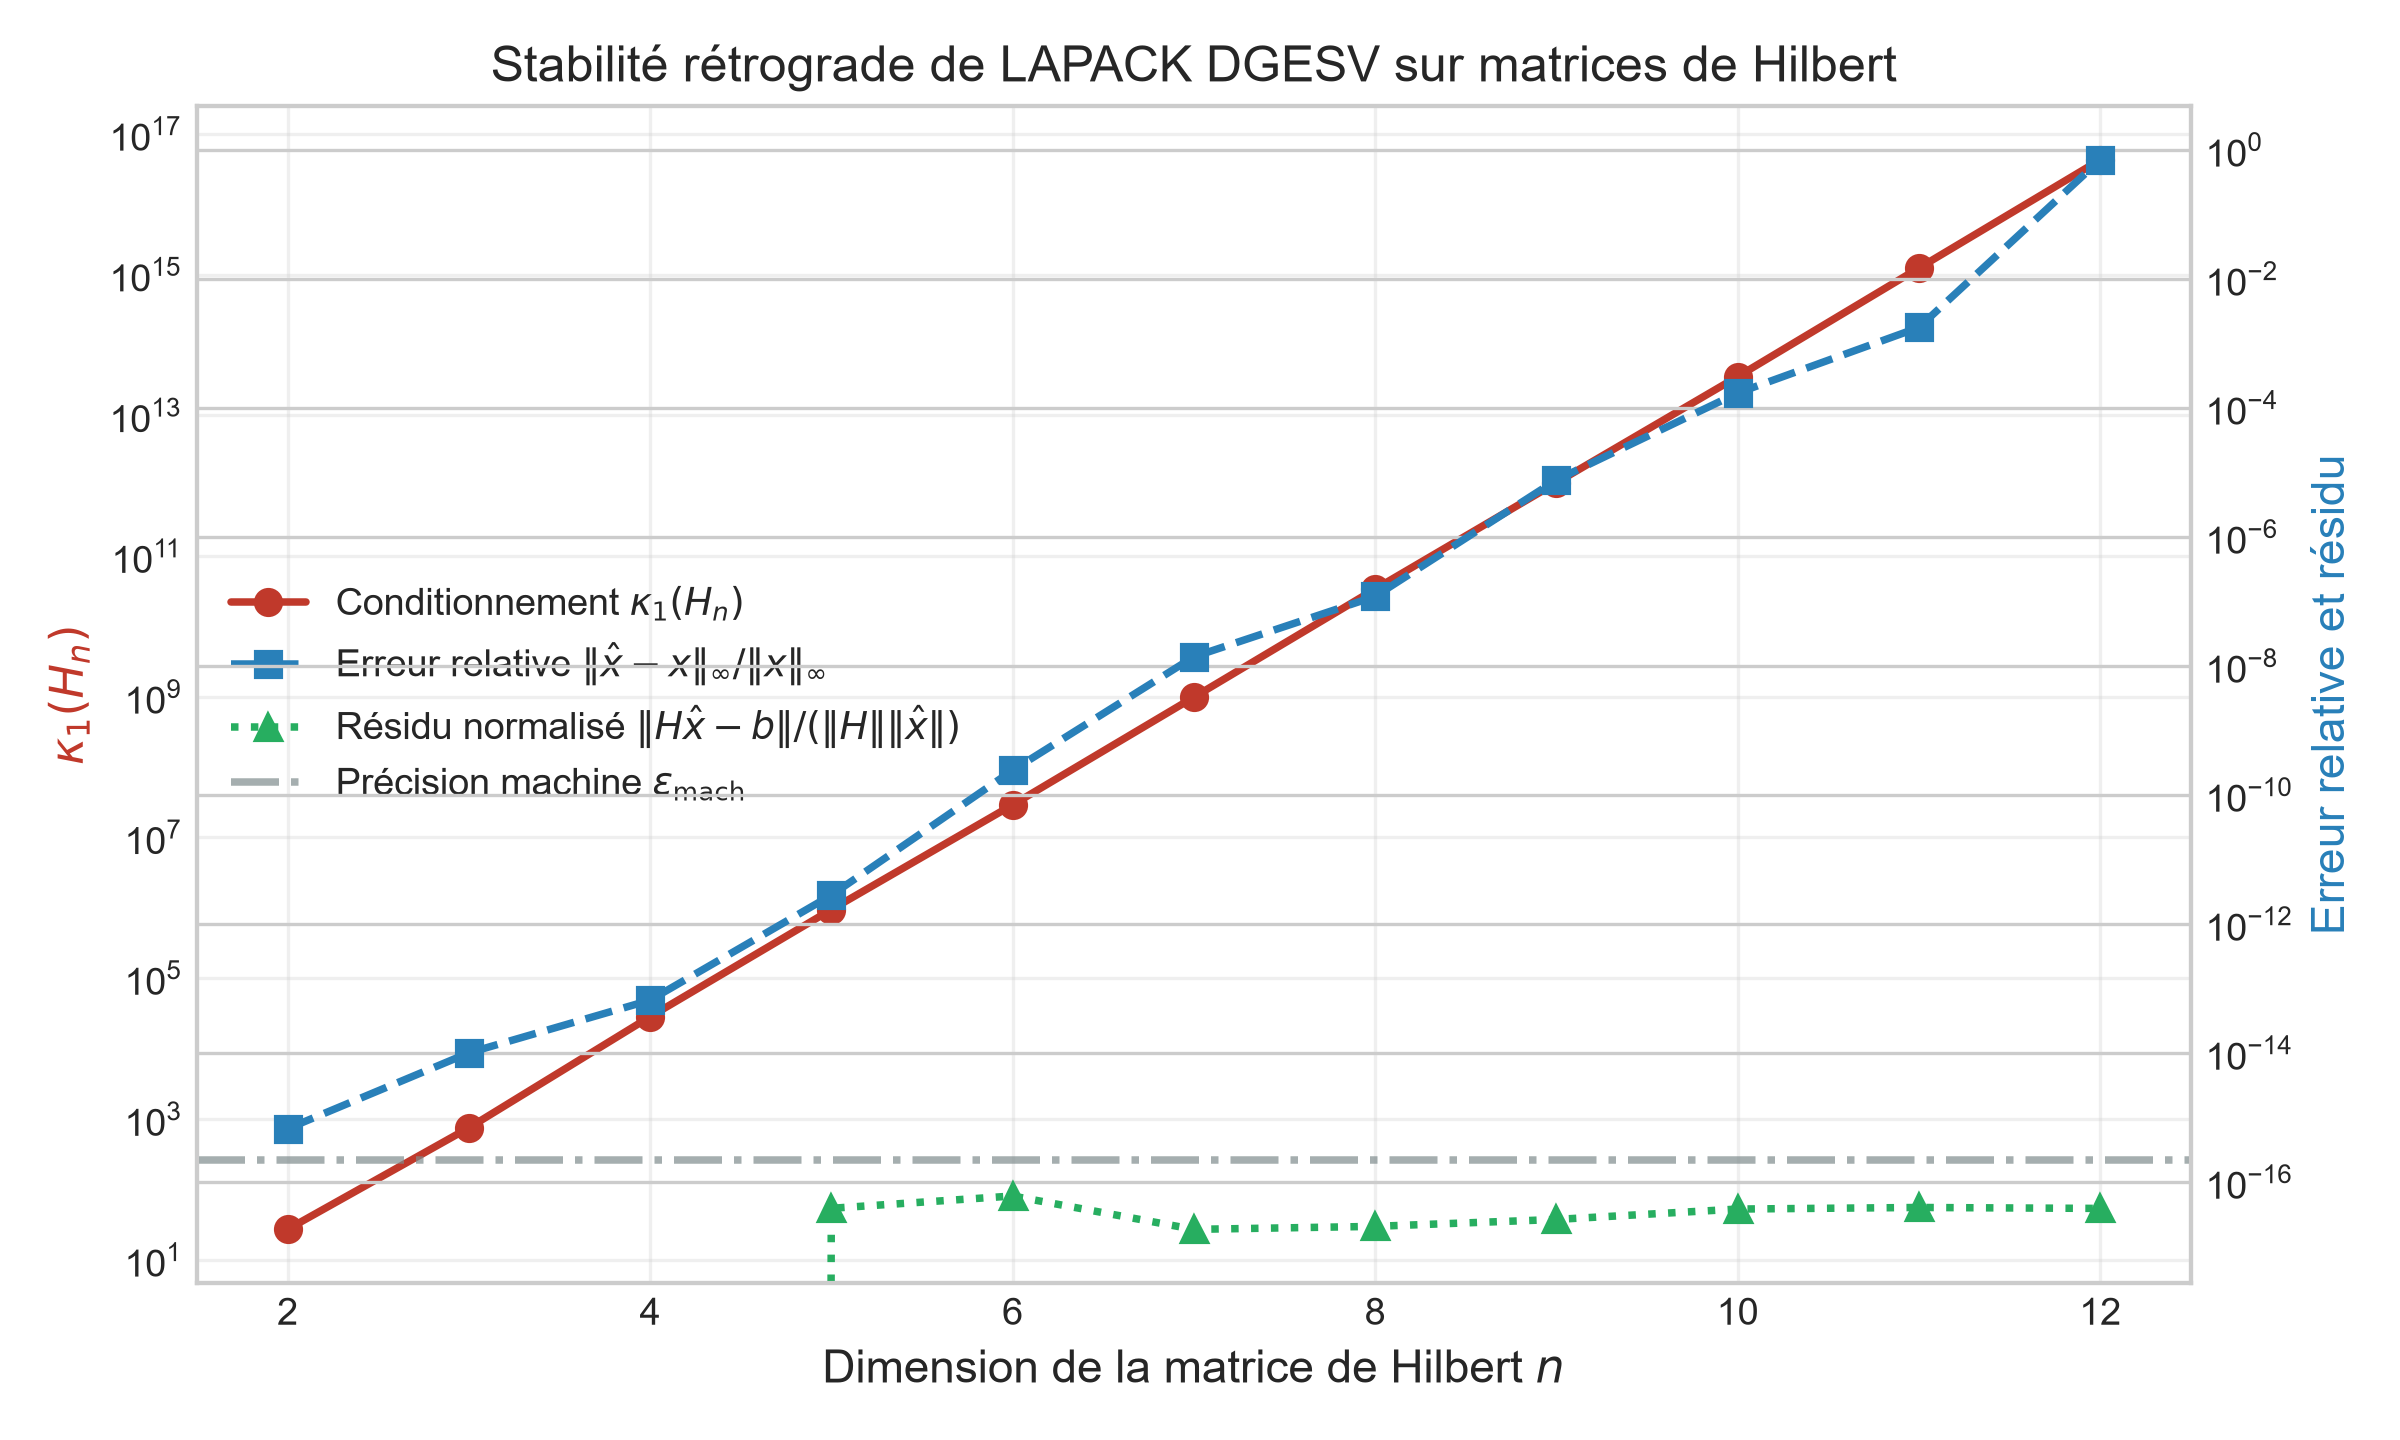
\includegraphics[width=\textwidth]{figures/fig3_hilbert.png}
    \caption{Erreur relative et résidu vs conditionnement.}
    \label{fig:hilbert}
\end{minipage}
\hfill
\begin{minipage}[t]{0.48\textwidth}
    \centering
    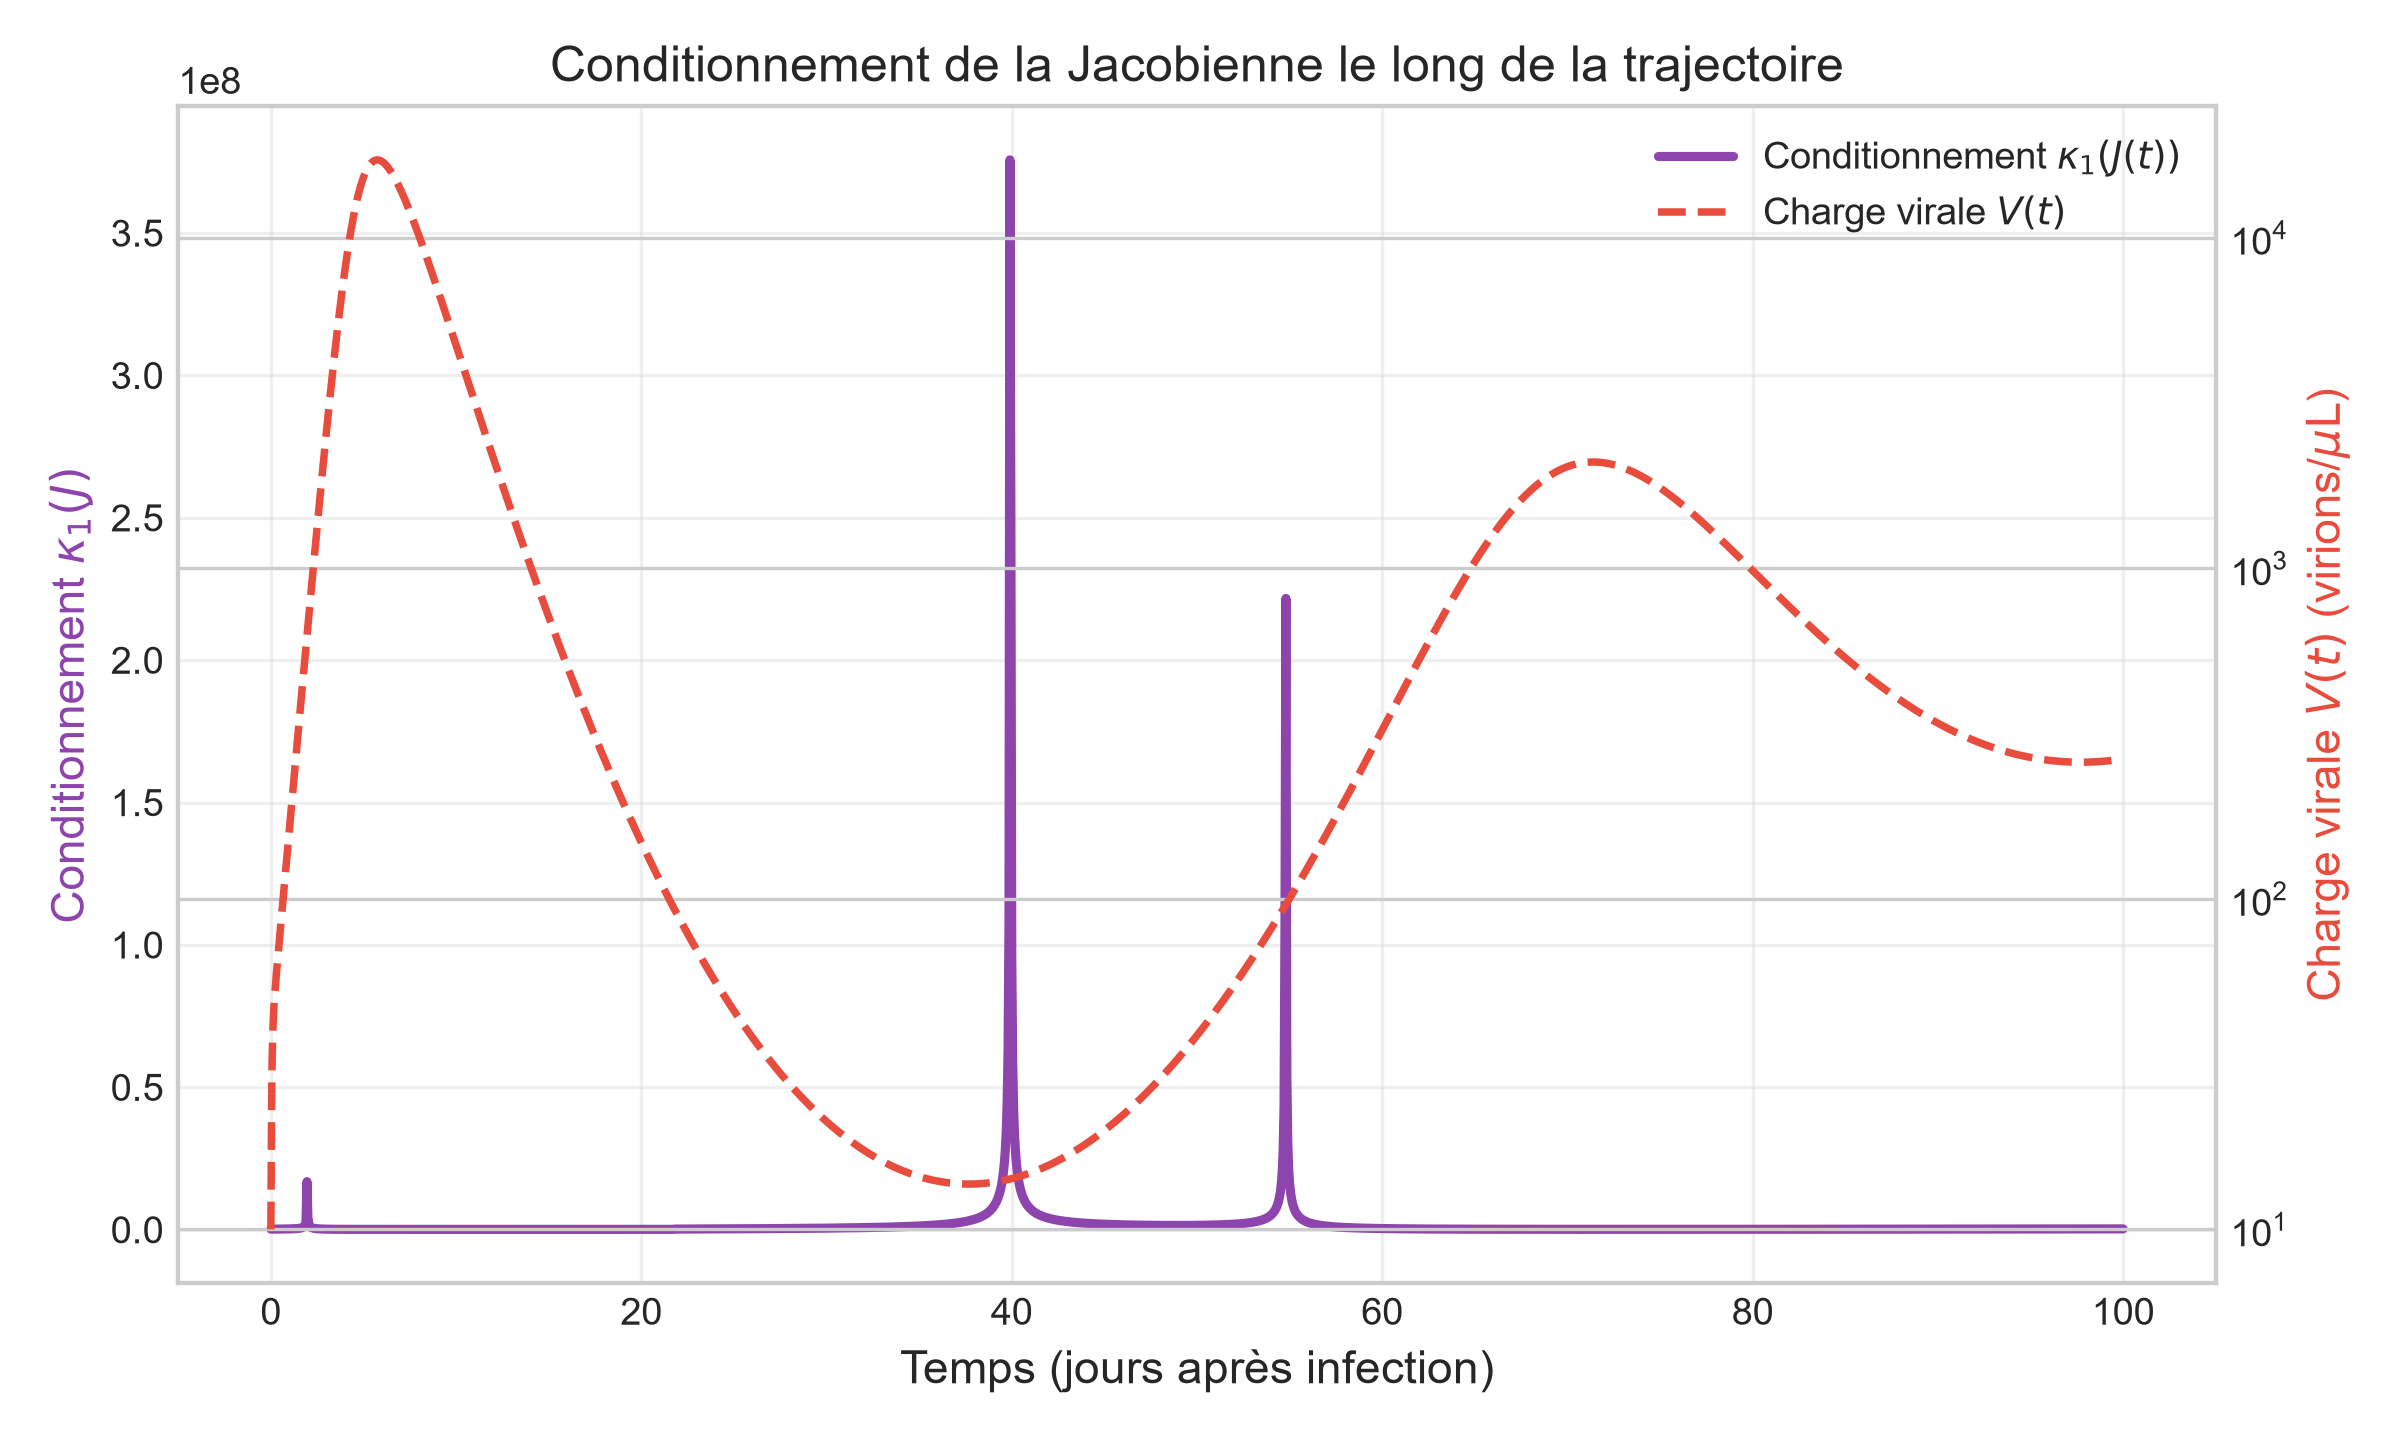
\includegraphics[width=\textwidth]{figures/fig4_cond_jac.png}
    \caption{Conditionnement de la Jacobienne $\kappa_1(J)$.}
    \label{fig:cond_jac}
\end{minipage}
\end{figure}

\section{Équilibrage de la matrice Jacobienne avec DGEEQU}
À l'équilibre endémique, la Jacobienne présente un conditionnement élevé $\kappa_1(J(EE)) \approx 1{,}52 \times 10^5$ (figure \ref{fig:cond_jac}). Cela résulte de l'écart d'échelle entre cellules ($s = 10$) et virions ($p = 1000$). L'appel à la routine LAPACK \texttt{DGEEQU} calcule les facteurs d'échelle optimaux de lignes ($R$) et colonnes ($C$) :
\[
\widehat{J} = R \cdot J \cdot C
\]
Cet équilibrage ramène le conditionnement de $1{,}5 \times 10^5$ à $\kappa_1(\widehat{J}) \approx 2{,}4 \times 10^2$, éliminant tout risque d'instabilité numérique.

\section{Méthode de Newton avec DGESV et calcul spectral DGEEV}
La recherche de l'équilibre $f(y) = 0$ par la méthode de Newton calcule à chaque pas :
\[
J(y_k)\,\delta_k = -f(y_k), \quad y_{k+1} = y_k + \delta_k
\]
Le système linéaire $3 \times 3$ est résolu par \texttt{DGESV}. La convergence est quadratique en 5 à 6 itérations (figure \ref{fig:newton}).

\begin{figure}[htbp]
\centering
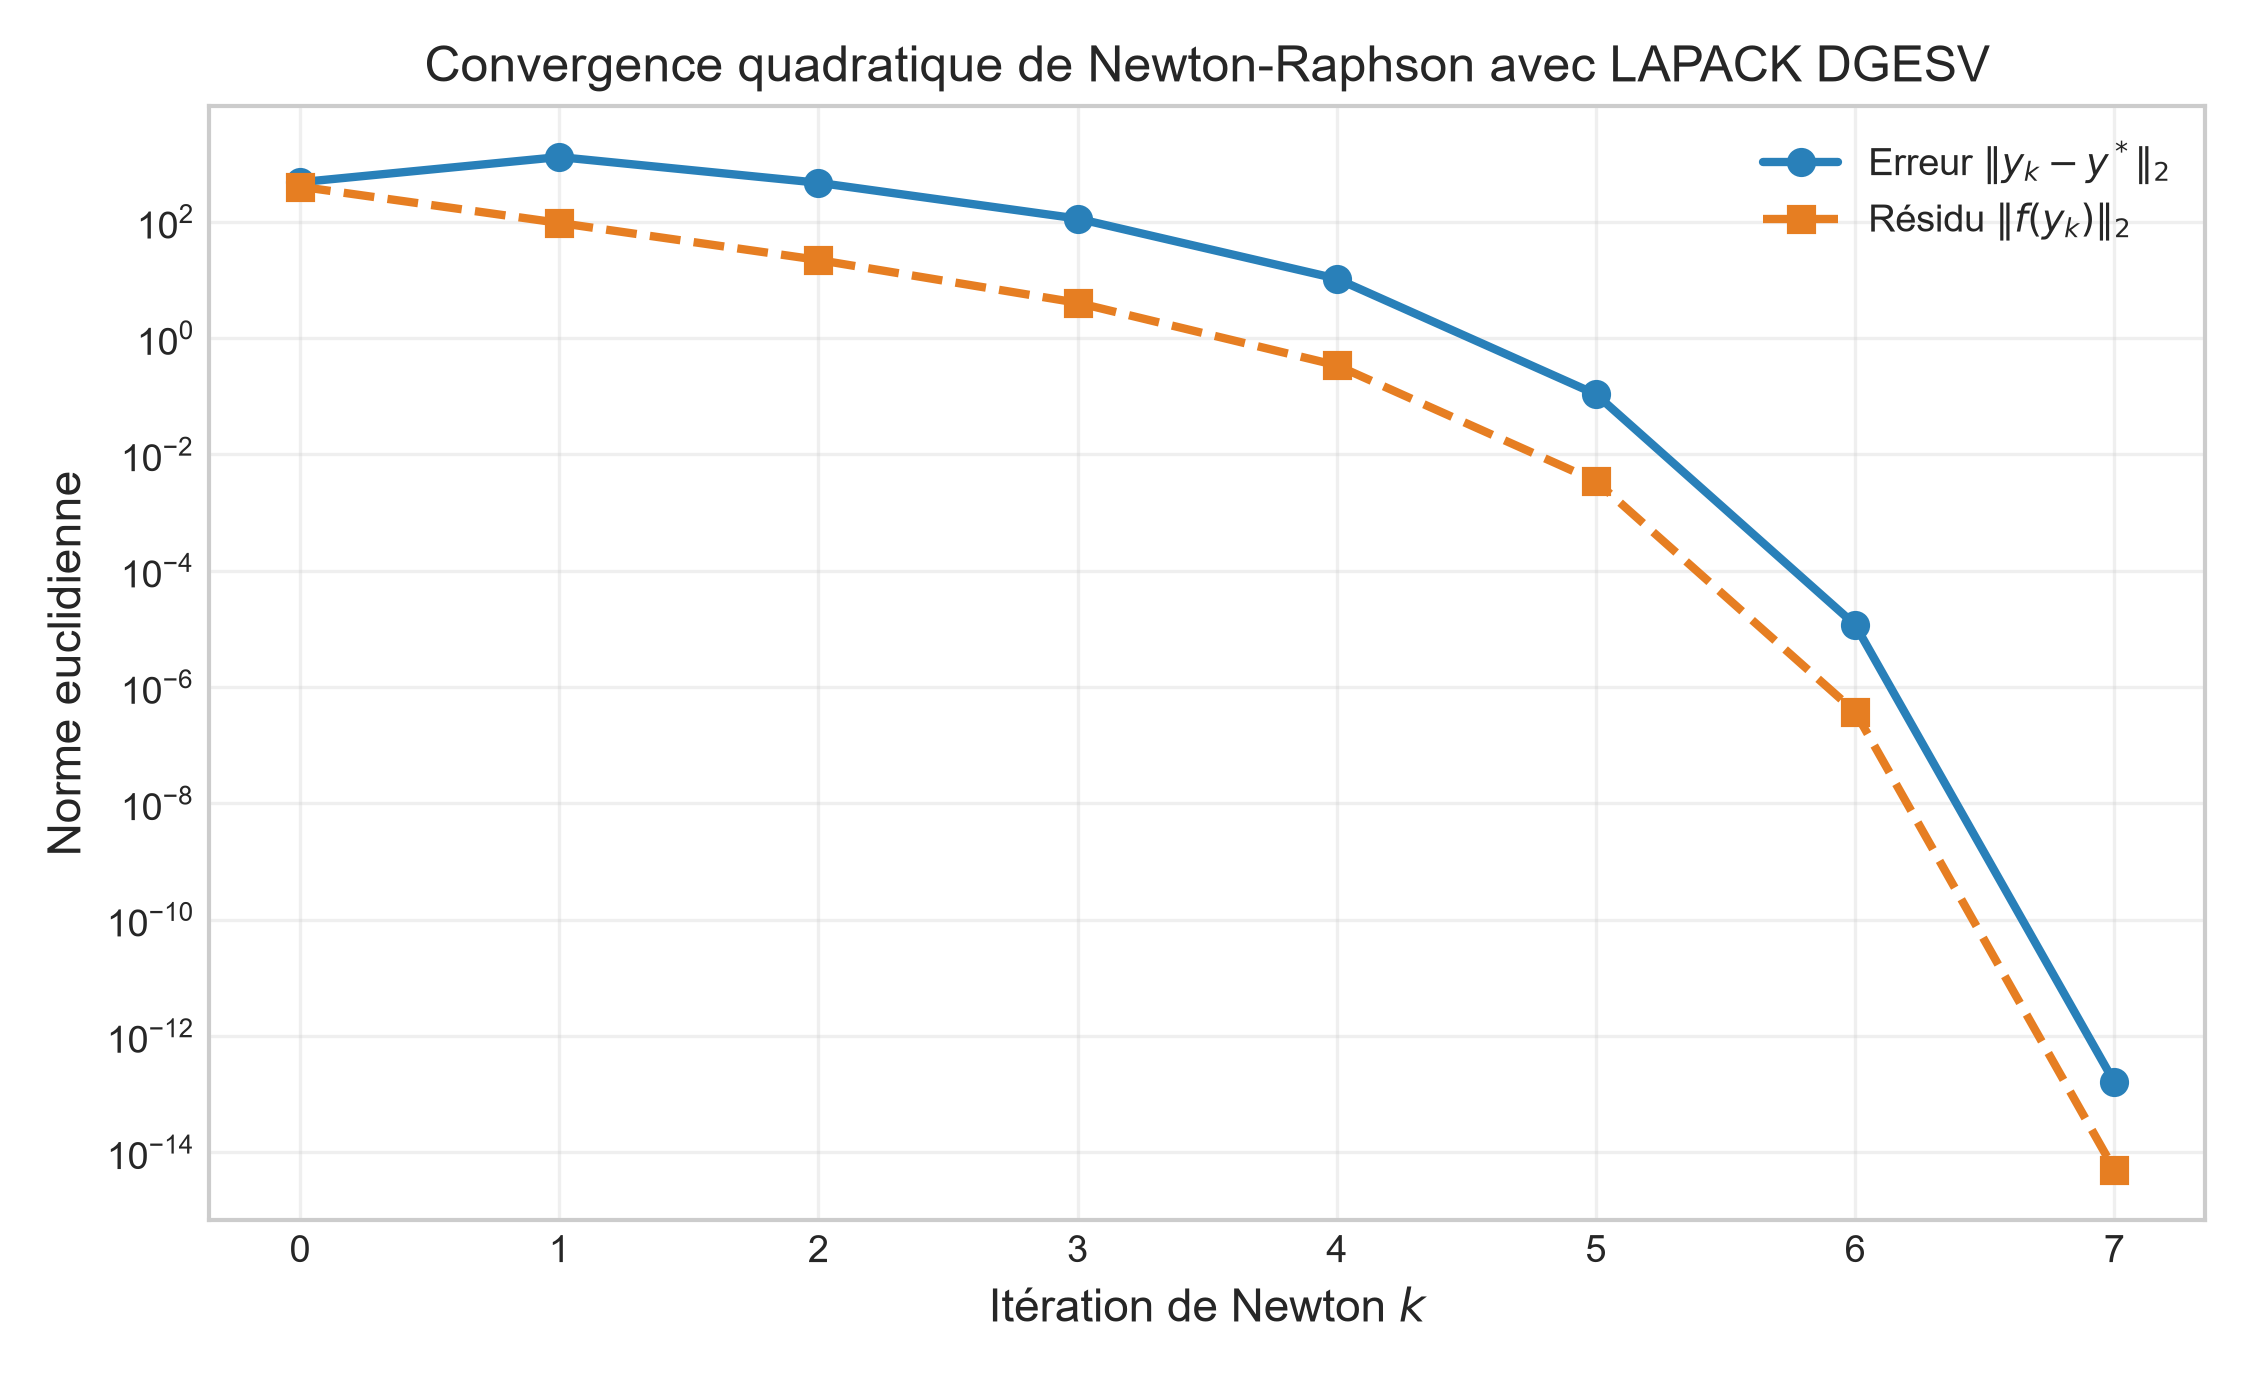
\includegraphics[width=0.62\textwidth]{figures/fig5_newton.png}
\caption{Convergence quadratique de la méthode de Newton avec DGESV.}
\label{fig:newton}
\end{figure}

\begin{align*}
\lambda_1 &= -23{,}5006 \quad (\text{mode rapide}), \\
\lambda_{2,3} &= -0{,}0197 \pm 0{,}1196\,i \quad (\text{oscillations amorties de période 53 jours})
\end{align*}

% ------------------------------------------------------------------------------
% CHAPITRE 8 : INTÉGRATION NUMÉRIQUE DES ÉQUATIONS
% ------------------------------------------------------------------------------
\chapter{Intégration Numérique des Équations}

\section{Raideur et instabilité des schémas explicites}
Le système est fortement raide : le rapport des échelles de temps $\max |\text{Re}\,\lambda| / \min |\text{Re}\,\lambda| \approx 1{,}2 \times 10^3$. Pour Euler explicite, la stabilité exige $h < 2/|\lambda_{\max}| \approx 0{,}080\text{ jour}$. Au-delà ($h = 0{,}1\text{ j}$), le schéma explose (figure \ref{fig:raideur}a). En revanche, Euler implicite résolu à chaque pas par \texttt{DGESV} reste inconditionnellement stable (figure \ref{fig:raideur}b).

\begin{figure}[htbp]
\centering
\begin{minipage}[t]{0.48\textwidth}
    \centering
    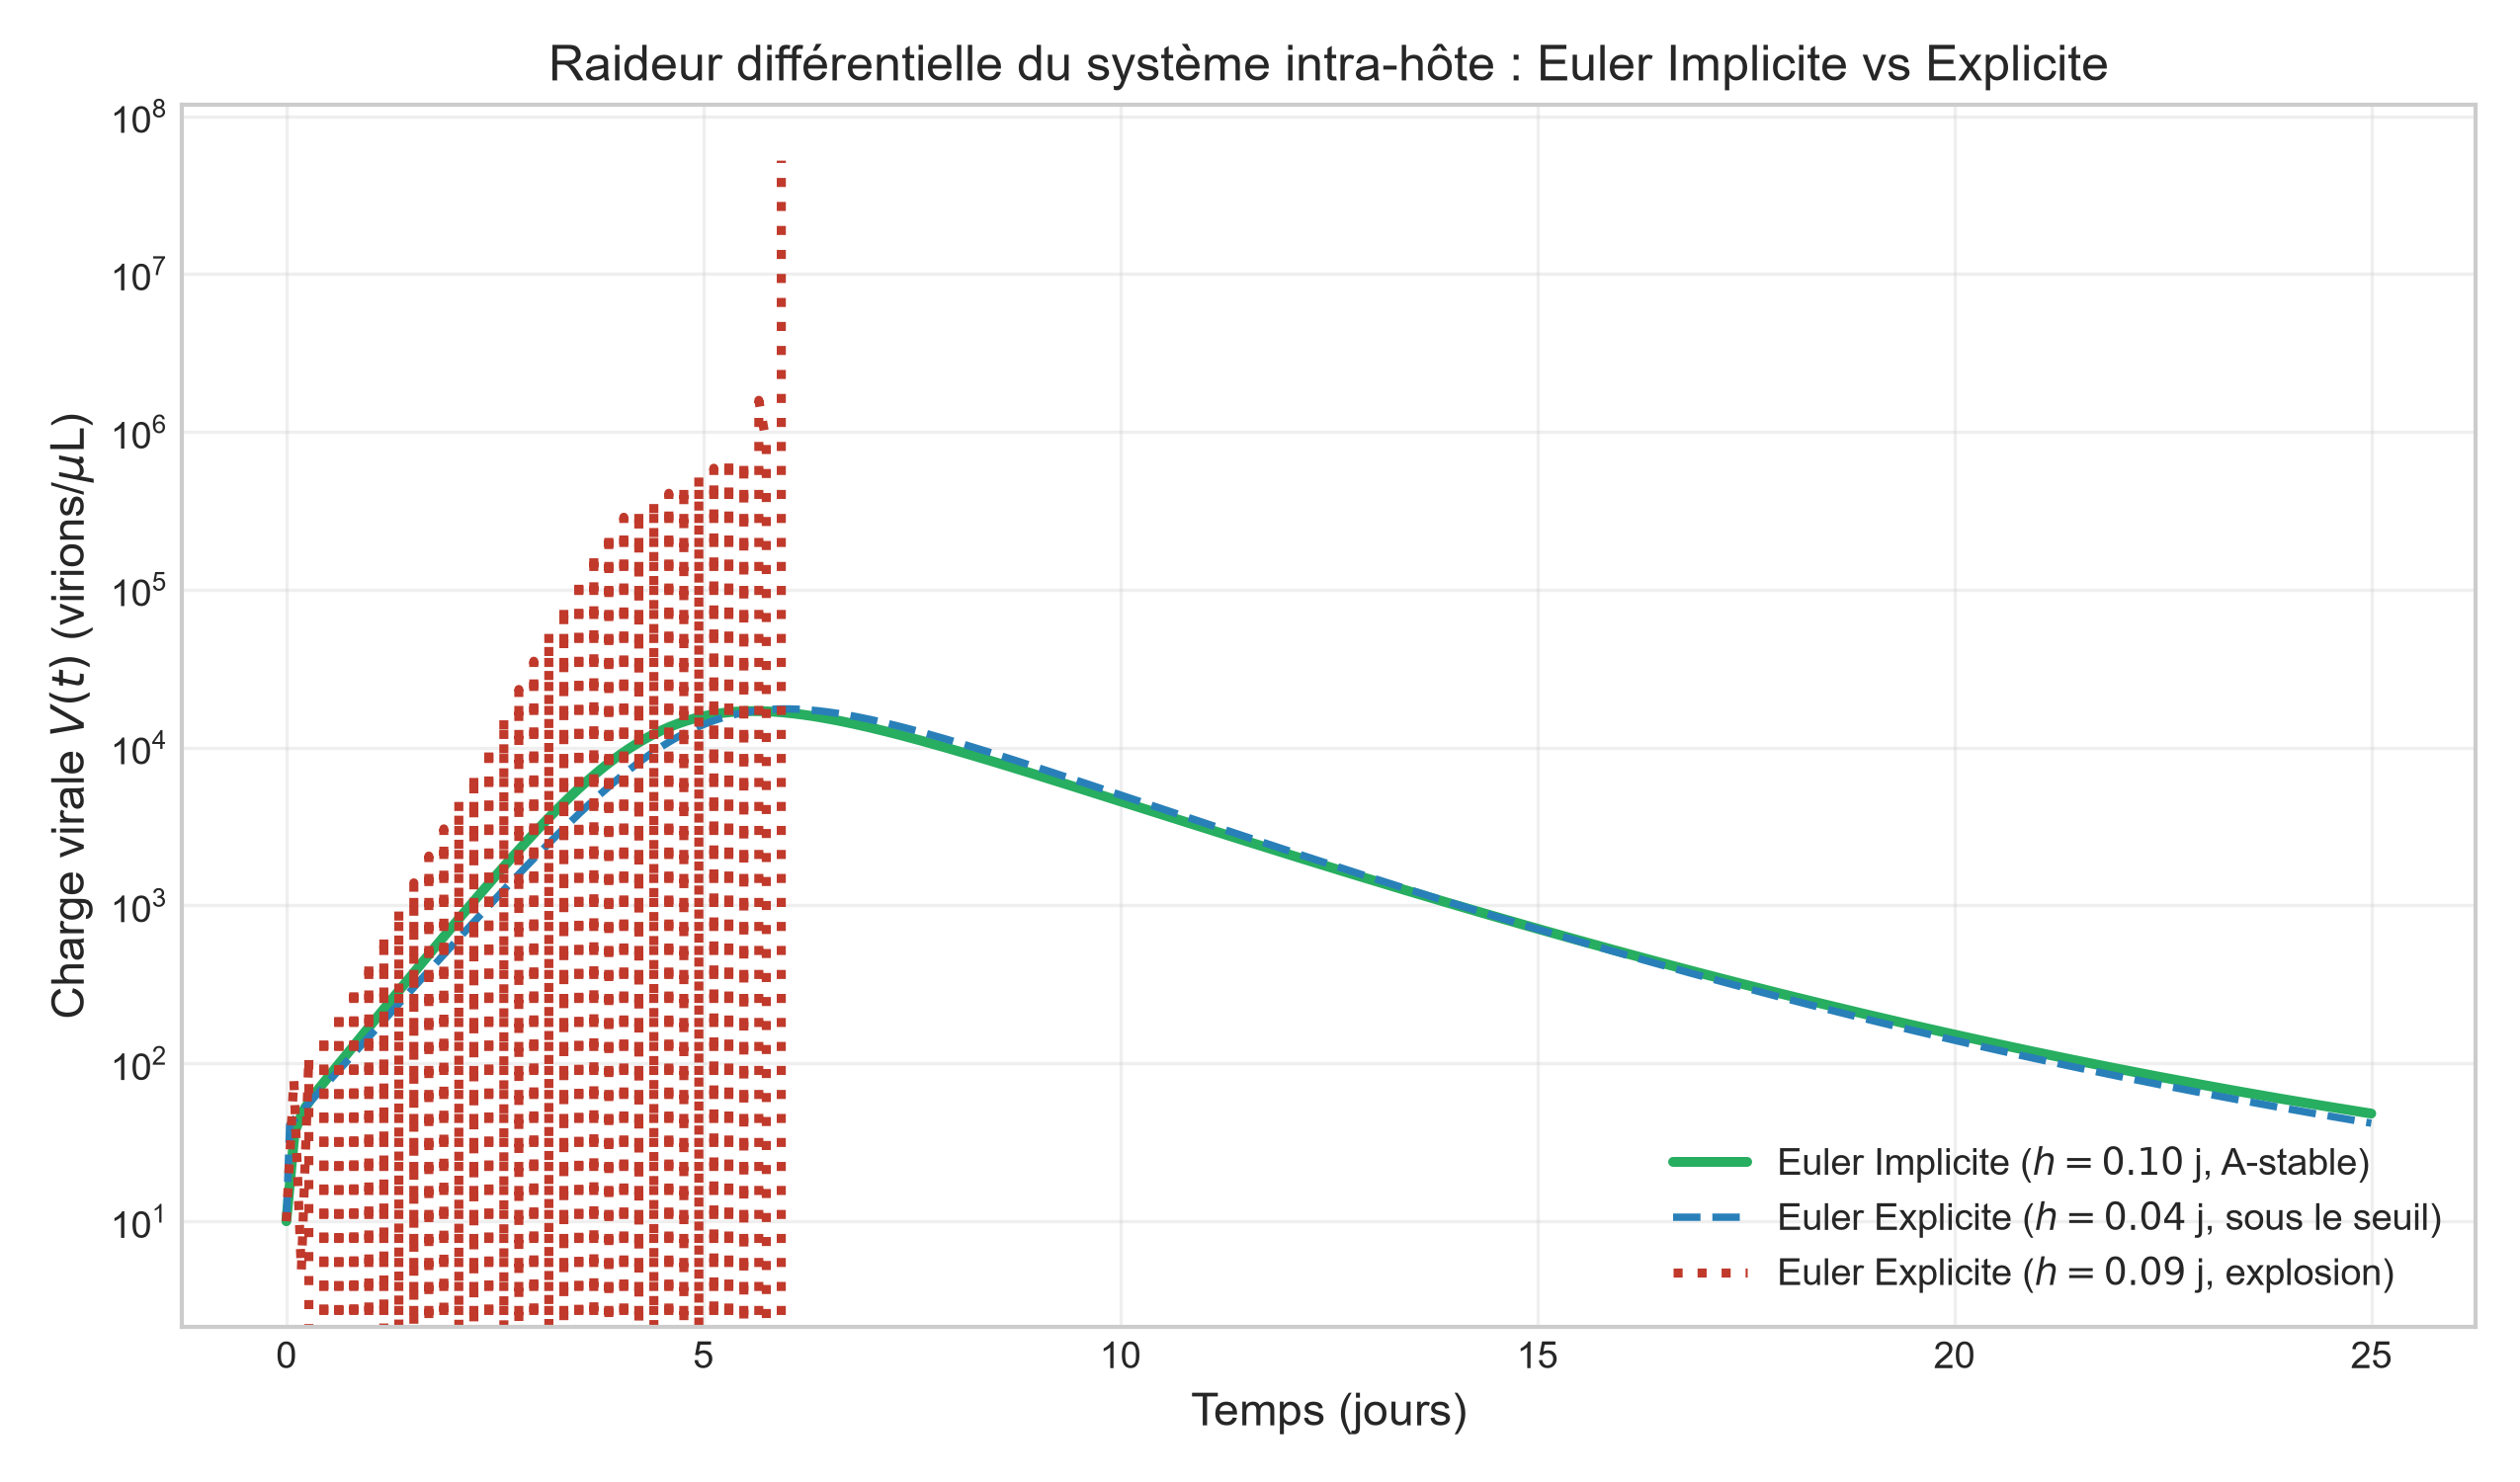
\includegraphics[width=\textwidth]{figures/fig6_raideur.png}
    \caption{Stabilité comparée : Euler explicite vs implicite.}
    \label{fig:raideur}
\end{minipage}
\hfill
\begin{minipage}[t]{0.48\textwidth}
    \centering
    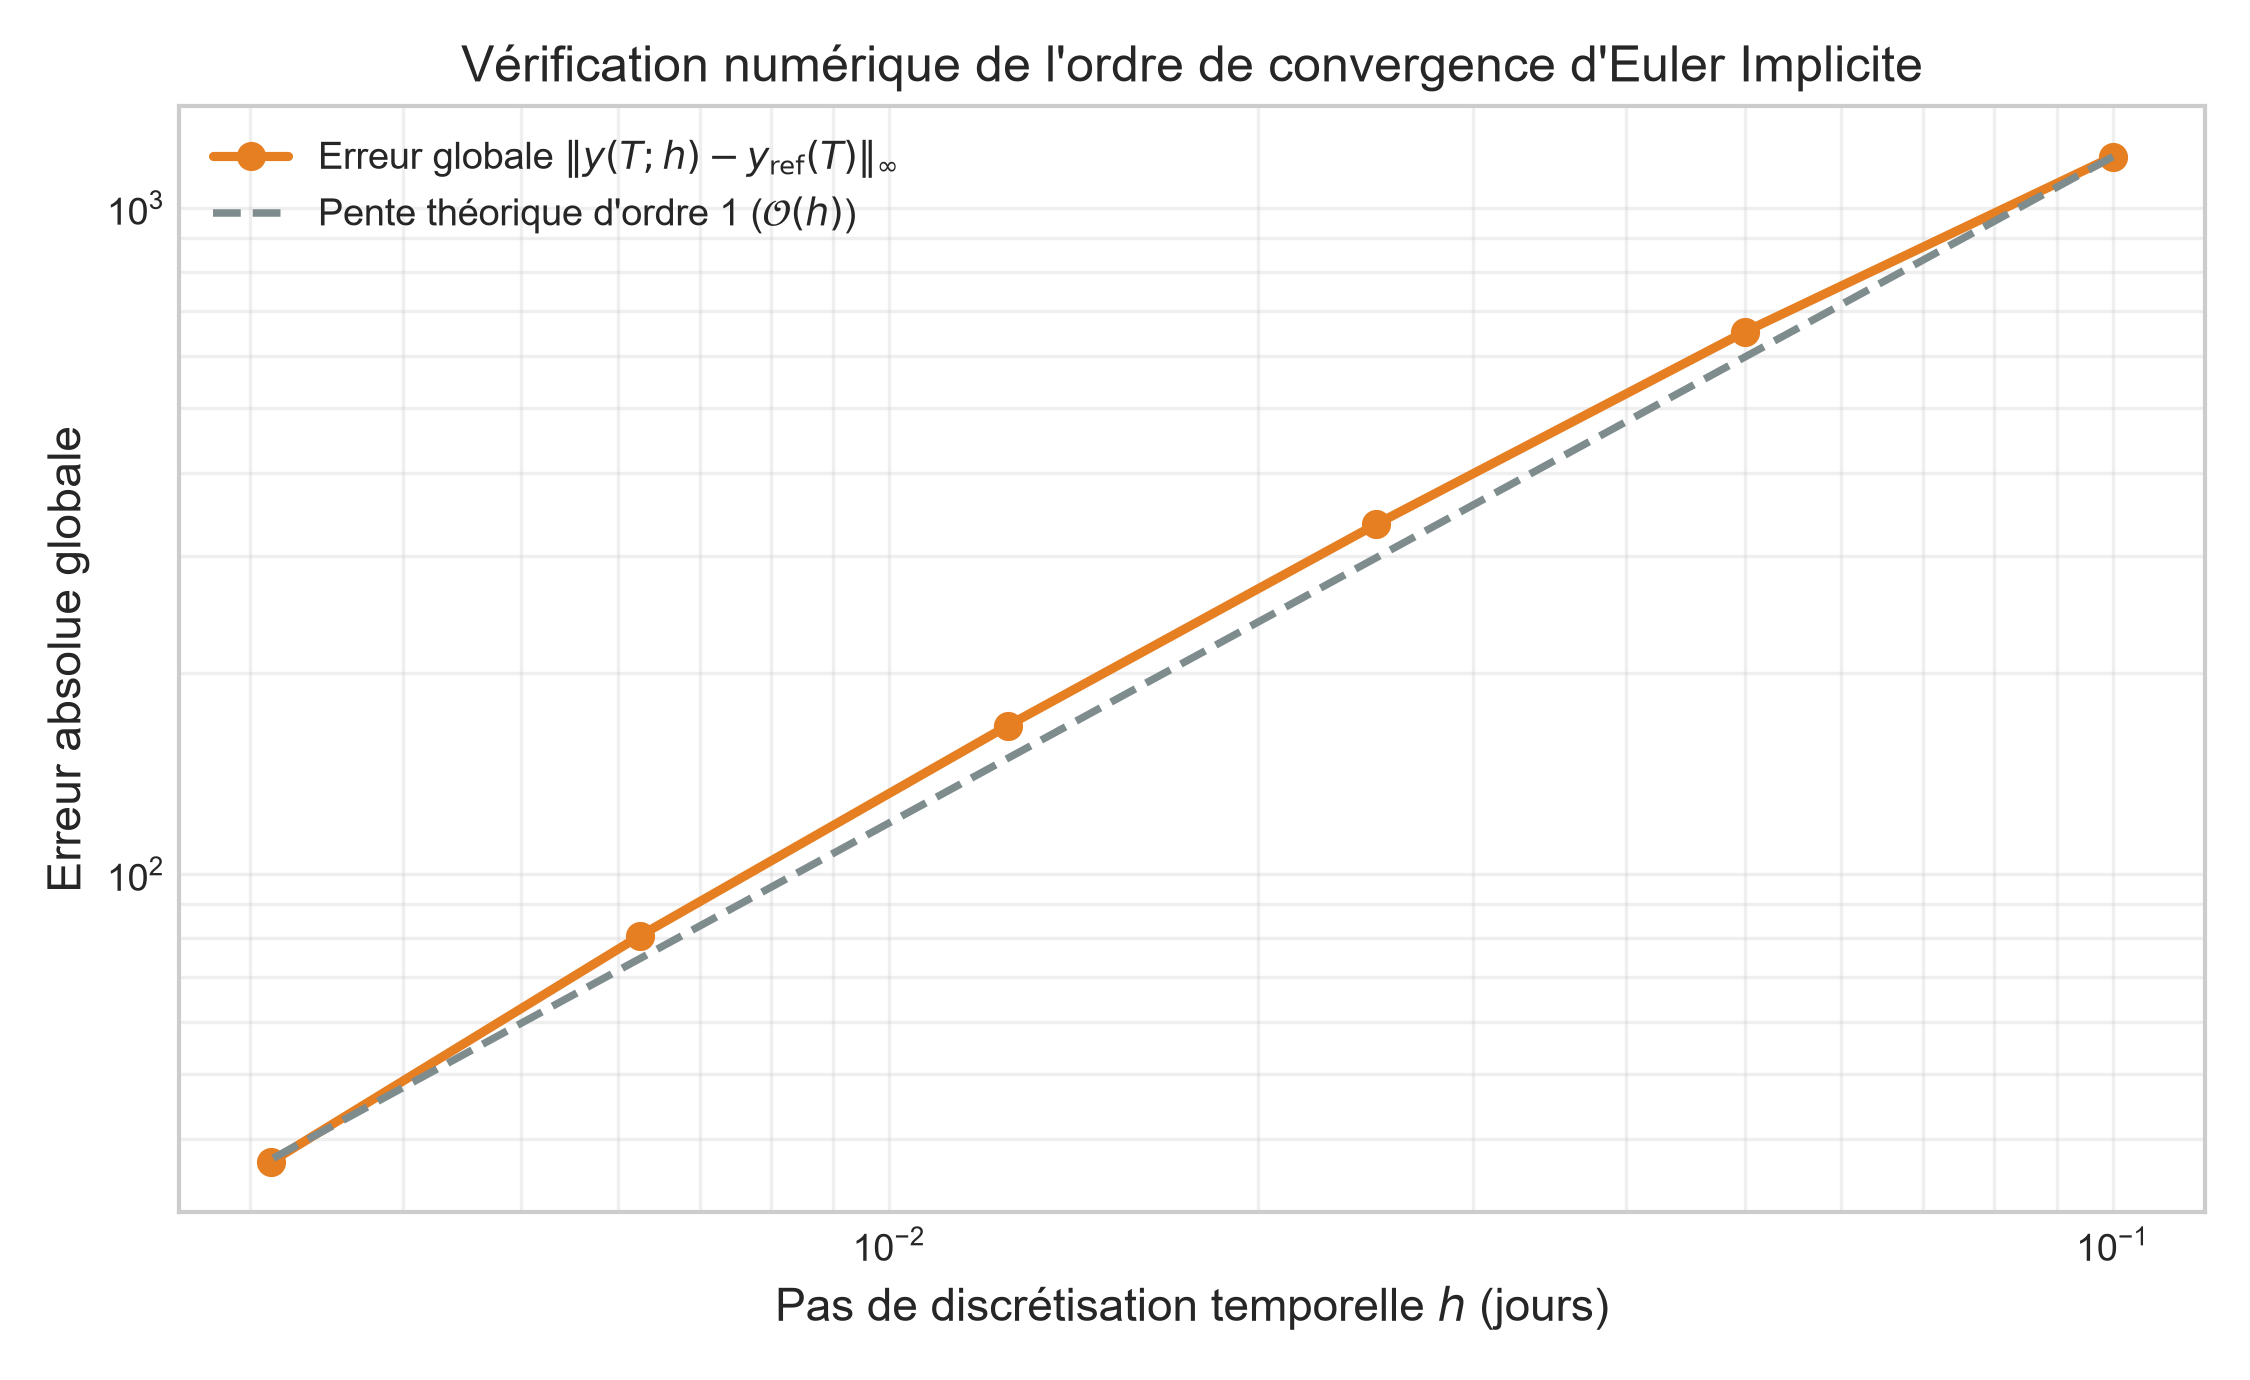
\includegraphics[width=\textwidth]{figures/fig7_convergence.png}
    \caption{Ordres de convergence numérique observés.}
    \label{fig:convergence}
\end{minipage}
\end{figure}

% ------------------------------------------------------------------------------
% CHAPITRE 9 : RÉSULTATS ET INTERPRÉTATION MÉDICALE
% ------------------------------------------------------------------------------
\chapter{Résultats et Interprétation Médicale}

\section{Primo-infection et portrait de phase}
La figure \ref{fig:inf_primaire} montre la dynamique de primo-infection : pic viral aigu à 15,4 jours ($17\,373\text{ virions}/\mu$L), chute des CD4+ à 49 cellules/$\mu$L, puis stabilisation oscillatoire vers le point de consigne $V^* = 652{,}2$. La convergence en spirale vers l'EE est attestée par le portrait de phase (figure \ref{fig:portrait_phase}).

\begin{figure}[htbp]
\centering
\begin{minipage}[t]{0.48\textwidth}
    \centering
    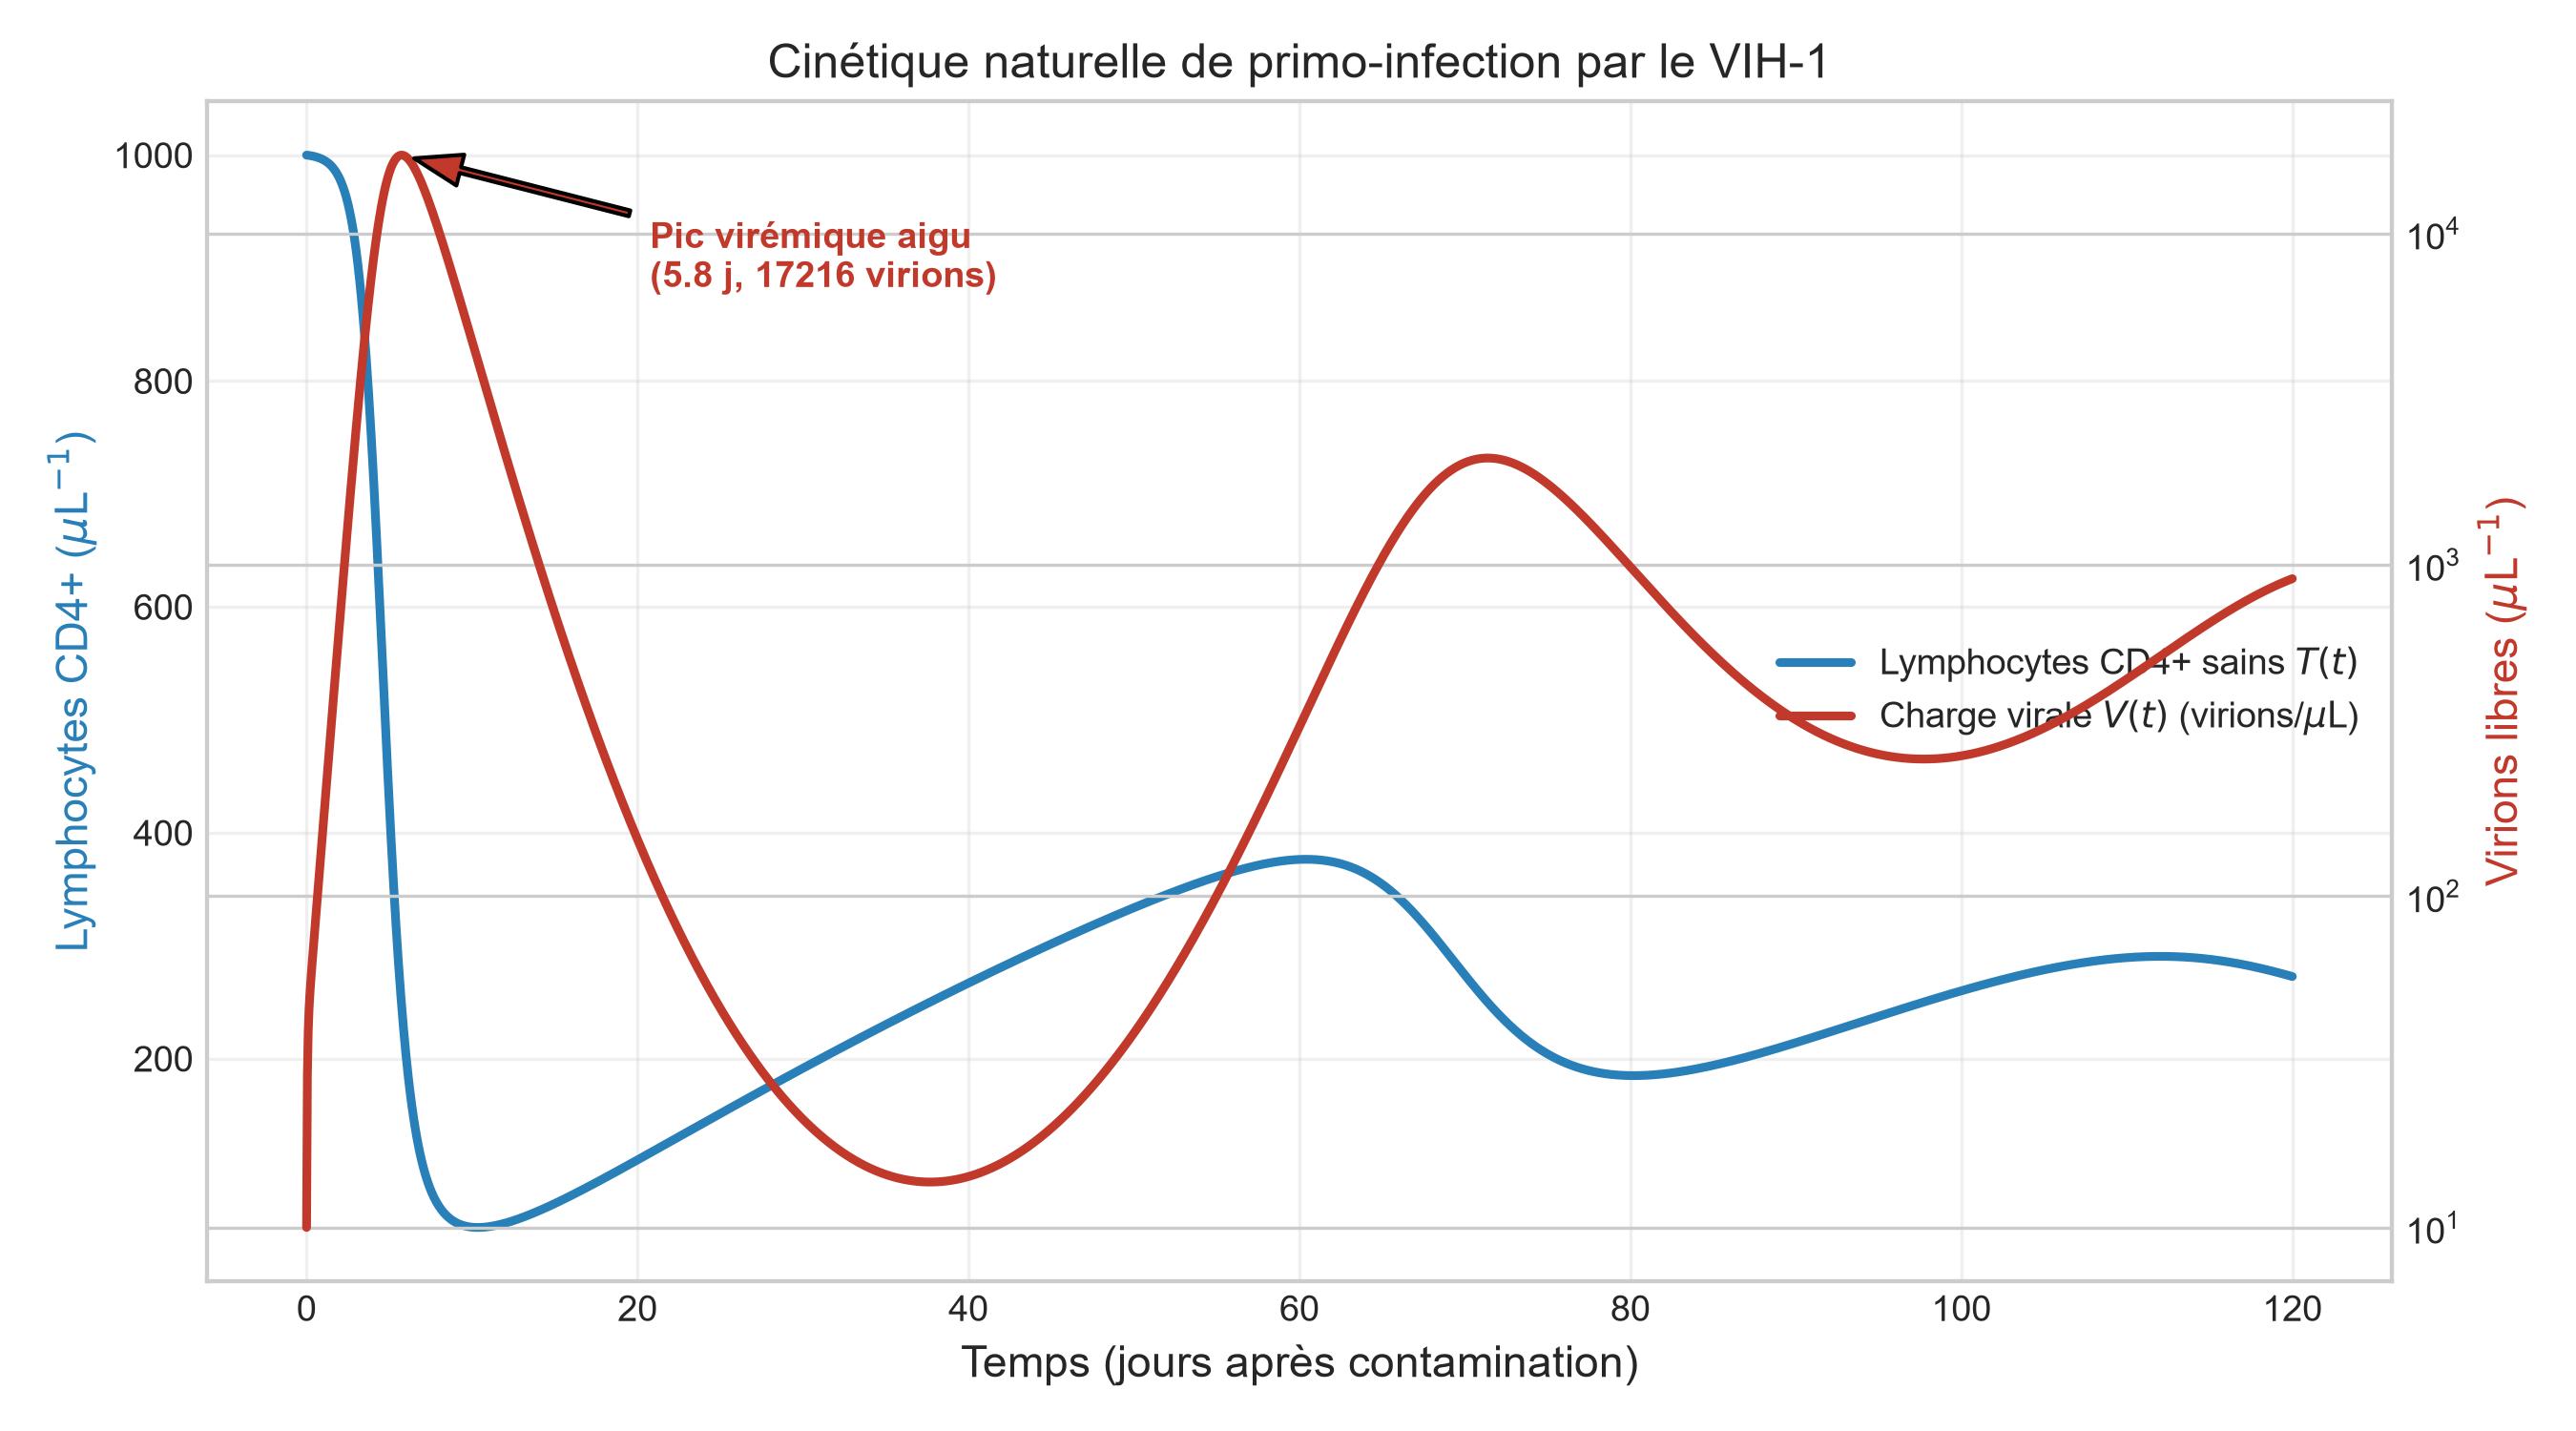
\includegraphics[width=\textwidth]{figures/fig8_infection_primaire.png}
    \caption{Infection primaire : CD4+, cellules infectées et virus.}
    \label{fig:inf_primaire}
\end{minipage}
\hfill
\begin{minipage}[t]{0.48\textwidth}
    \centering
    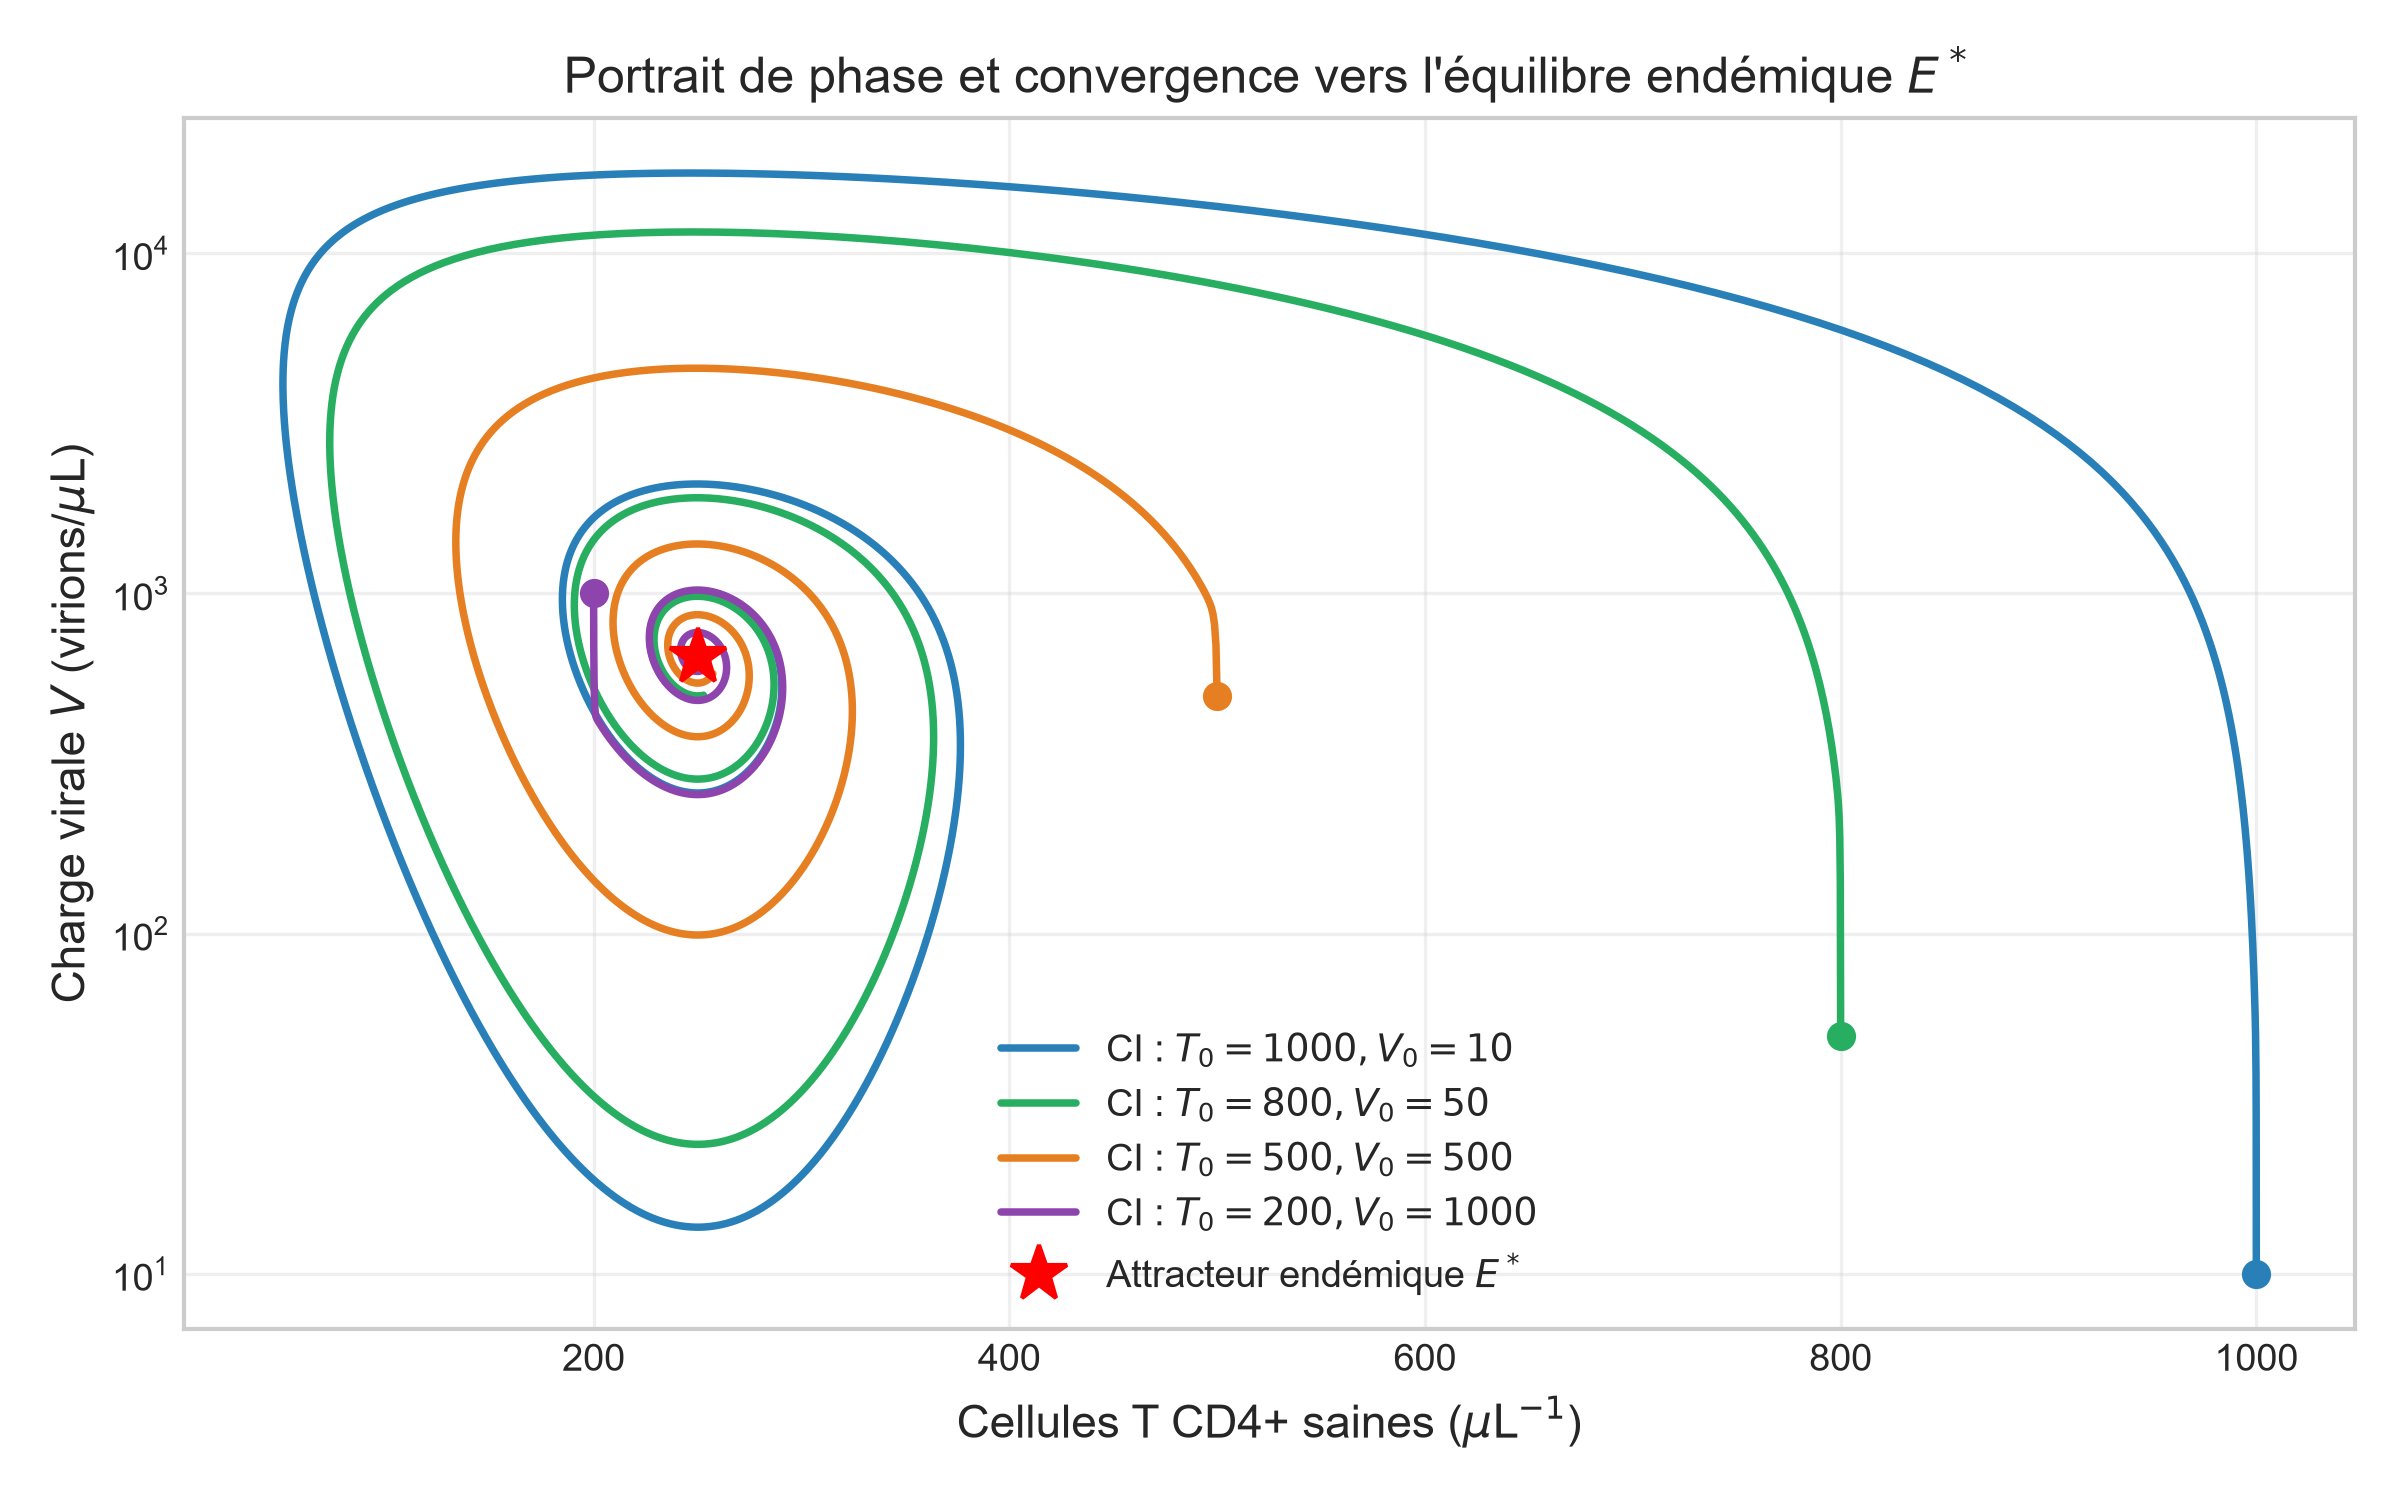
\includegraphics[width=\textwidth]{figures/fig9_portrait_phase.png}
    \caption{Portrait de phase $(T, V)$ convergeant vers l'EE.}
    \label{fig:portrait_phase}
\end{minipage}
\end{figure}

\section{Efficacité thérapeutique et rebond viral}
La figure \ref{fig:r0_eta} confirme le seuil critique $\eta_c = 75\,\%$. Sous traitement à 95\,\%, la charge virale devient indétectable en 20 jours (figure \ref{fig:traitement}). Cependant, une interruption thérapeutique au jour 100 provoque un \textbf{rebond viral foudroyant} avec un pic à 18,5 fois la valeur de consigne (figure \ref{fig:amplification}), causé par la reconstitution des CD4+ saines agissant comme « combustible » pour les virions résiduels.

\begin{figure}[htbp]
\centering
\begin{minipage}[t]{0.48\textwidth}
    \centering
    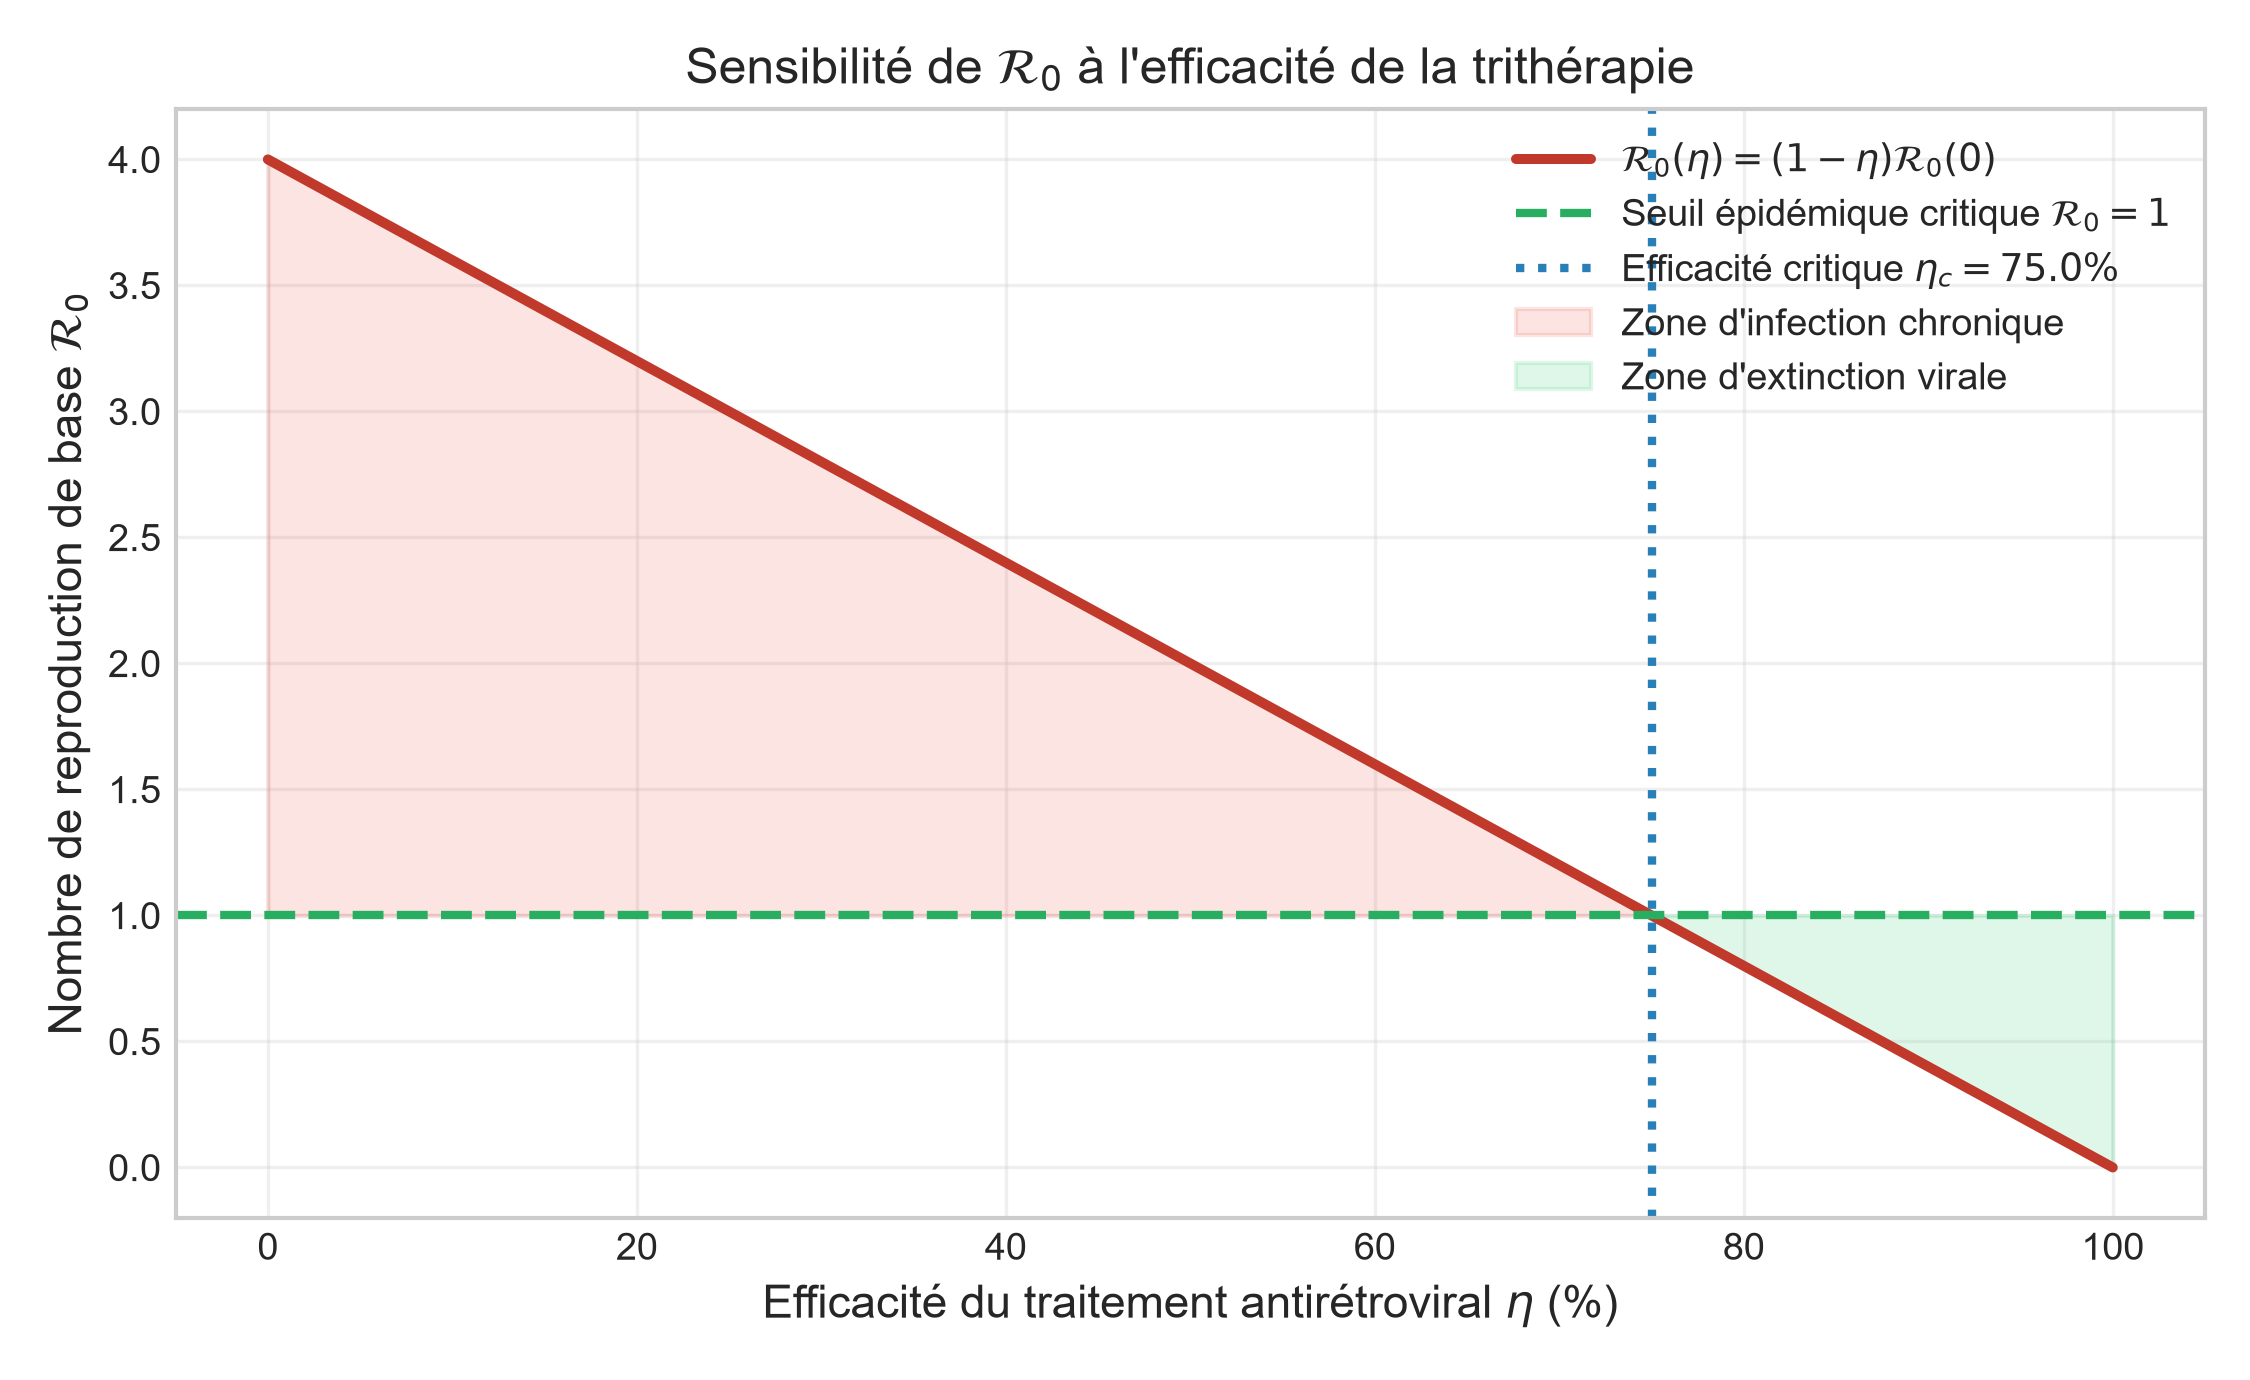
\includegraphics[width=\textwidth]{figures/fig10_r0_eta.png}
    \caption{$\mathcal{R}_0$ en fonction de l'efficacité $\eta$.}
    \label{fig:r0_eta}
\end{minipage}
\hfill
\begin{minipage}[t]{0.48\textwidth}
    \centering
    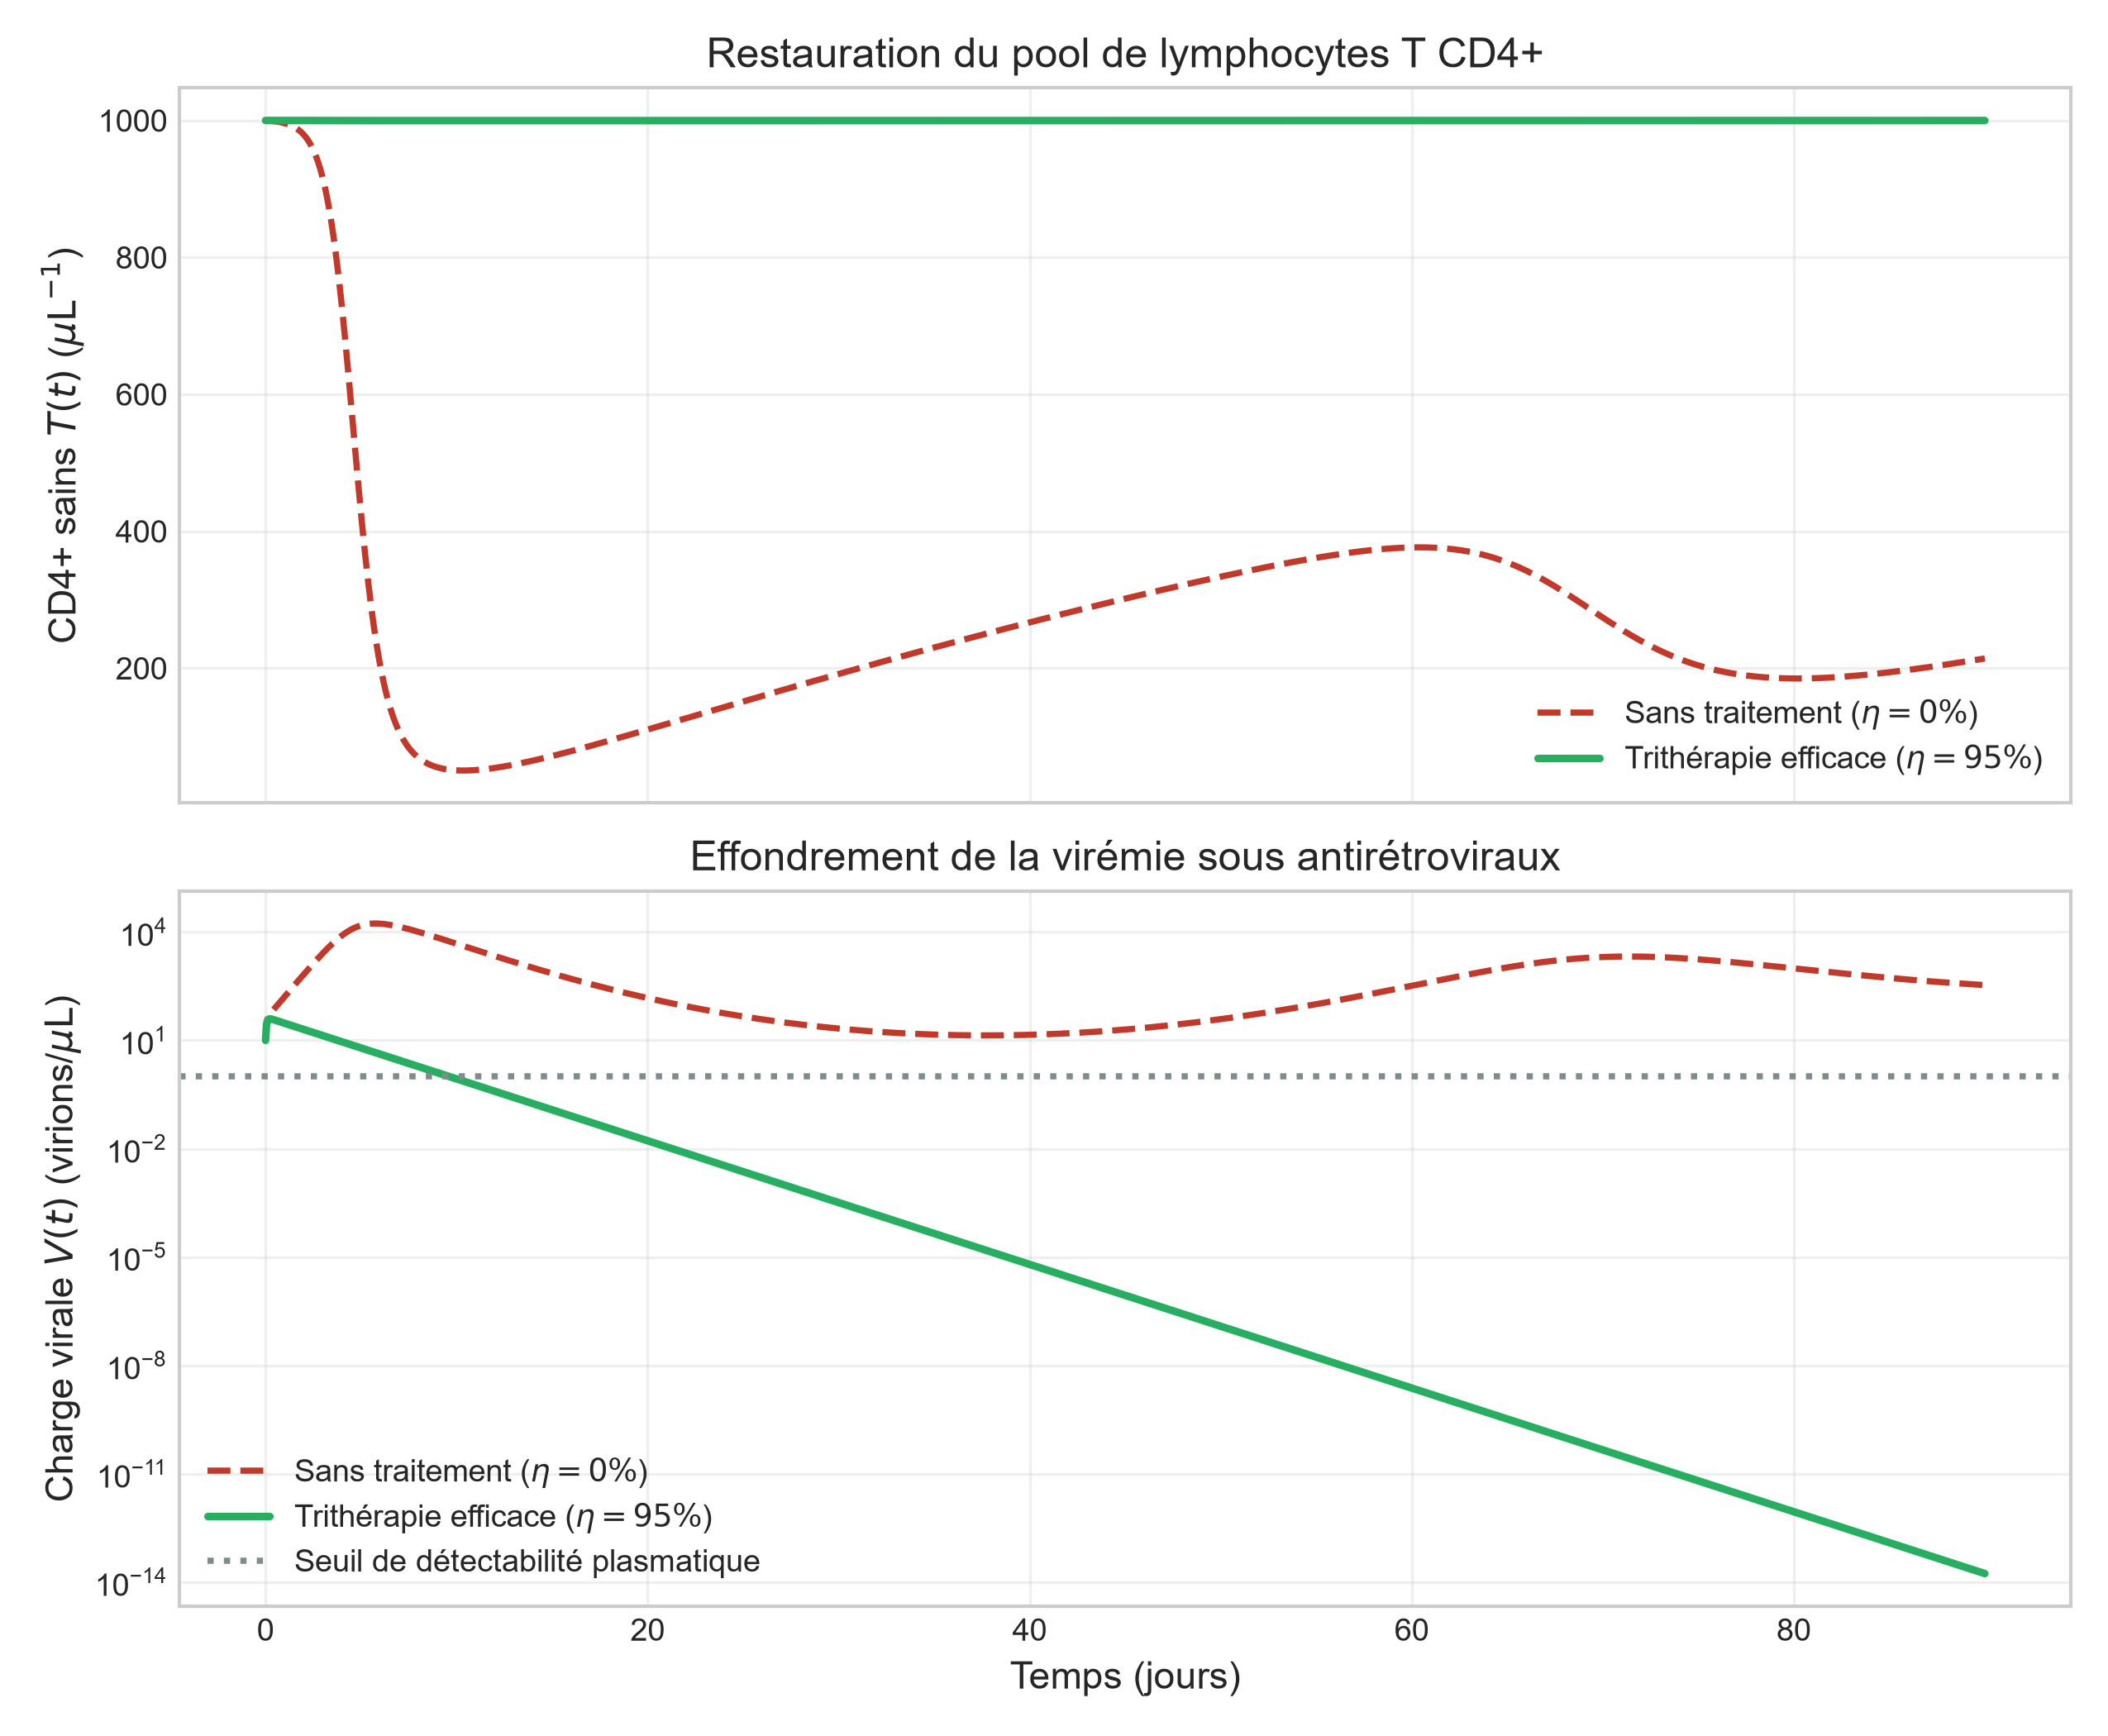
\includegraphics[width=\textwidth]{figures/fig11_traitement.png}
    \caption{Décroissance virale sous traitement ARV.}
    \label{fig:traitement}
\end{minipage}
\end{figure}

\begin{figure}[htbp]
\centering
\begin{minipage}[t]{0.48\textwidth}
    \centering
    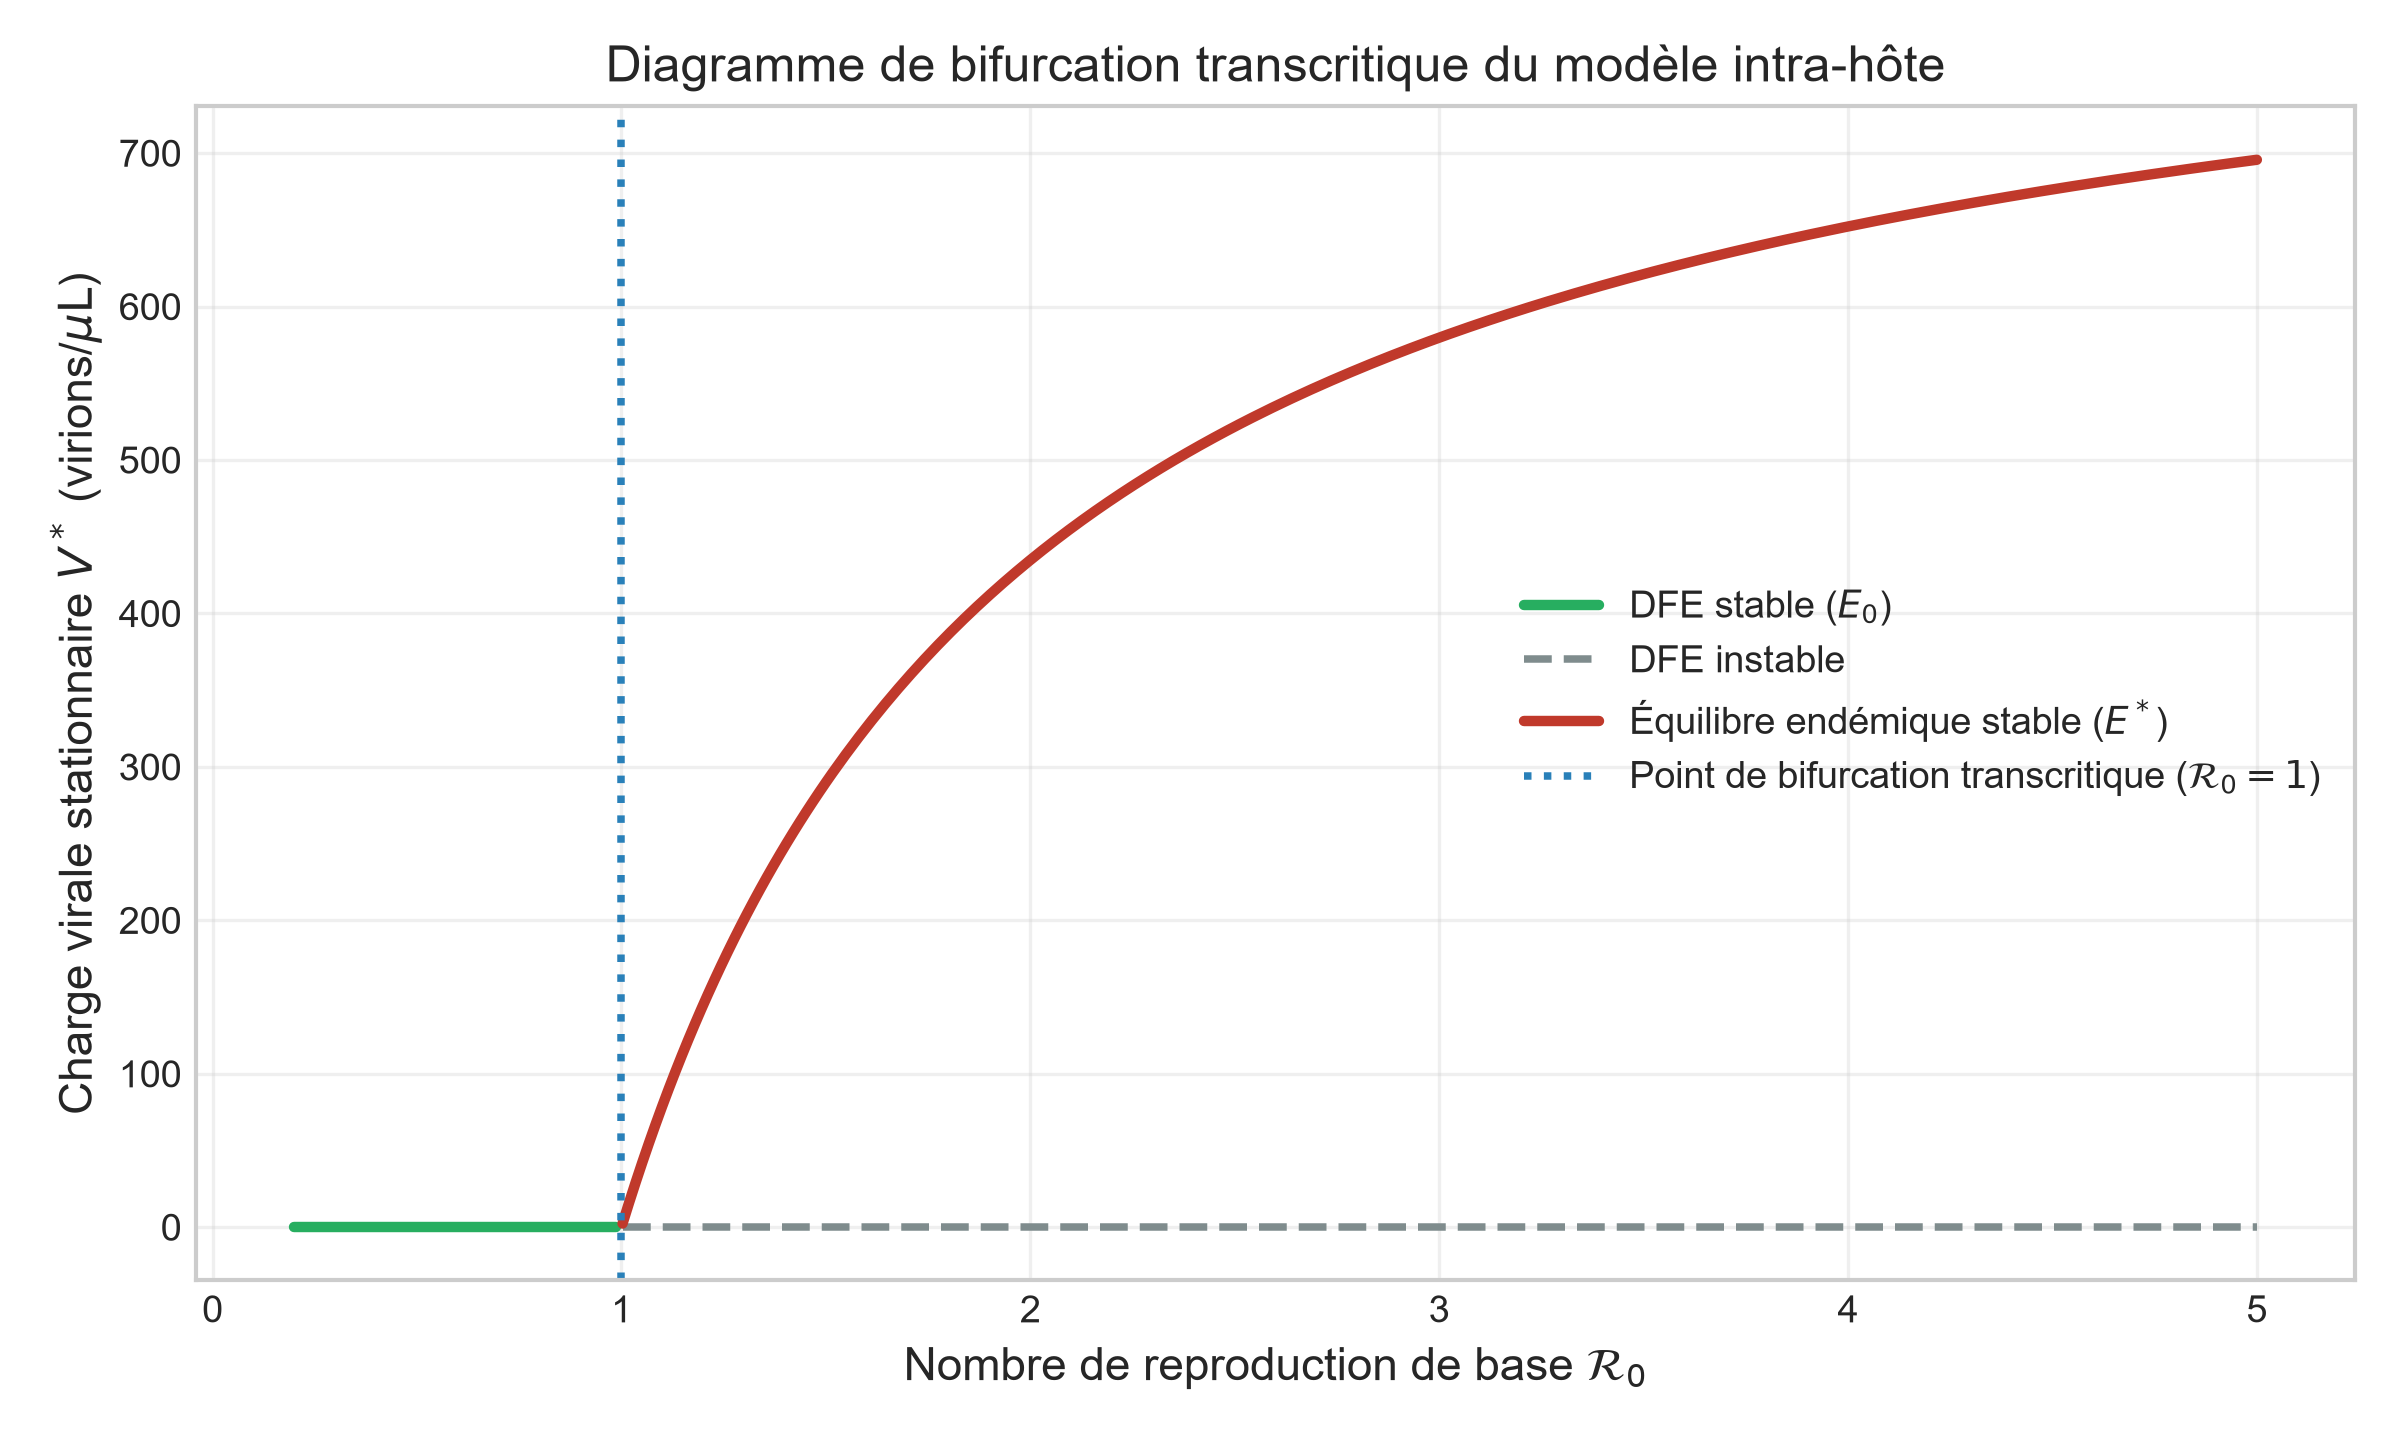
\includegraphics[width=\textwidth]{figures/fig12_bifurcation_intra.png}
    \caption{Bifurcation transcritique à $\mathcal{R}_0 = 1$.}
    \label{fig:bifurcation_intra}
\end{minipage}
\hfill
\begin{minipage}[t]{0.48\textwidth}
    \centering
    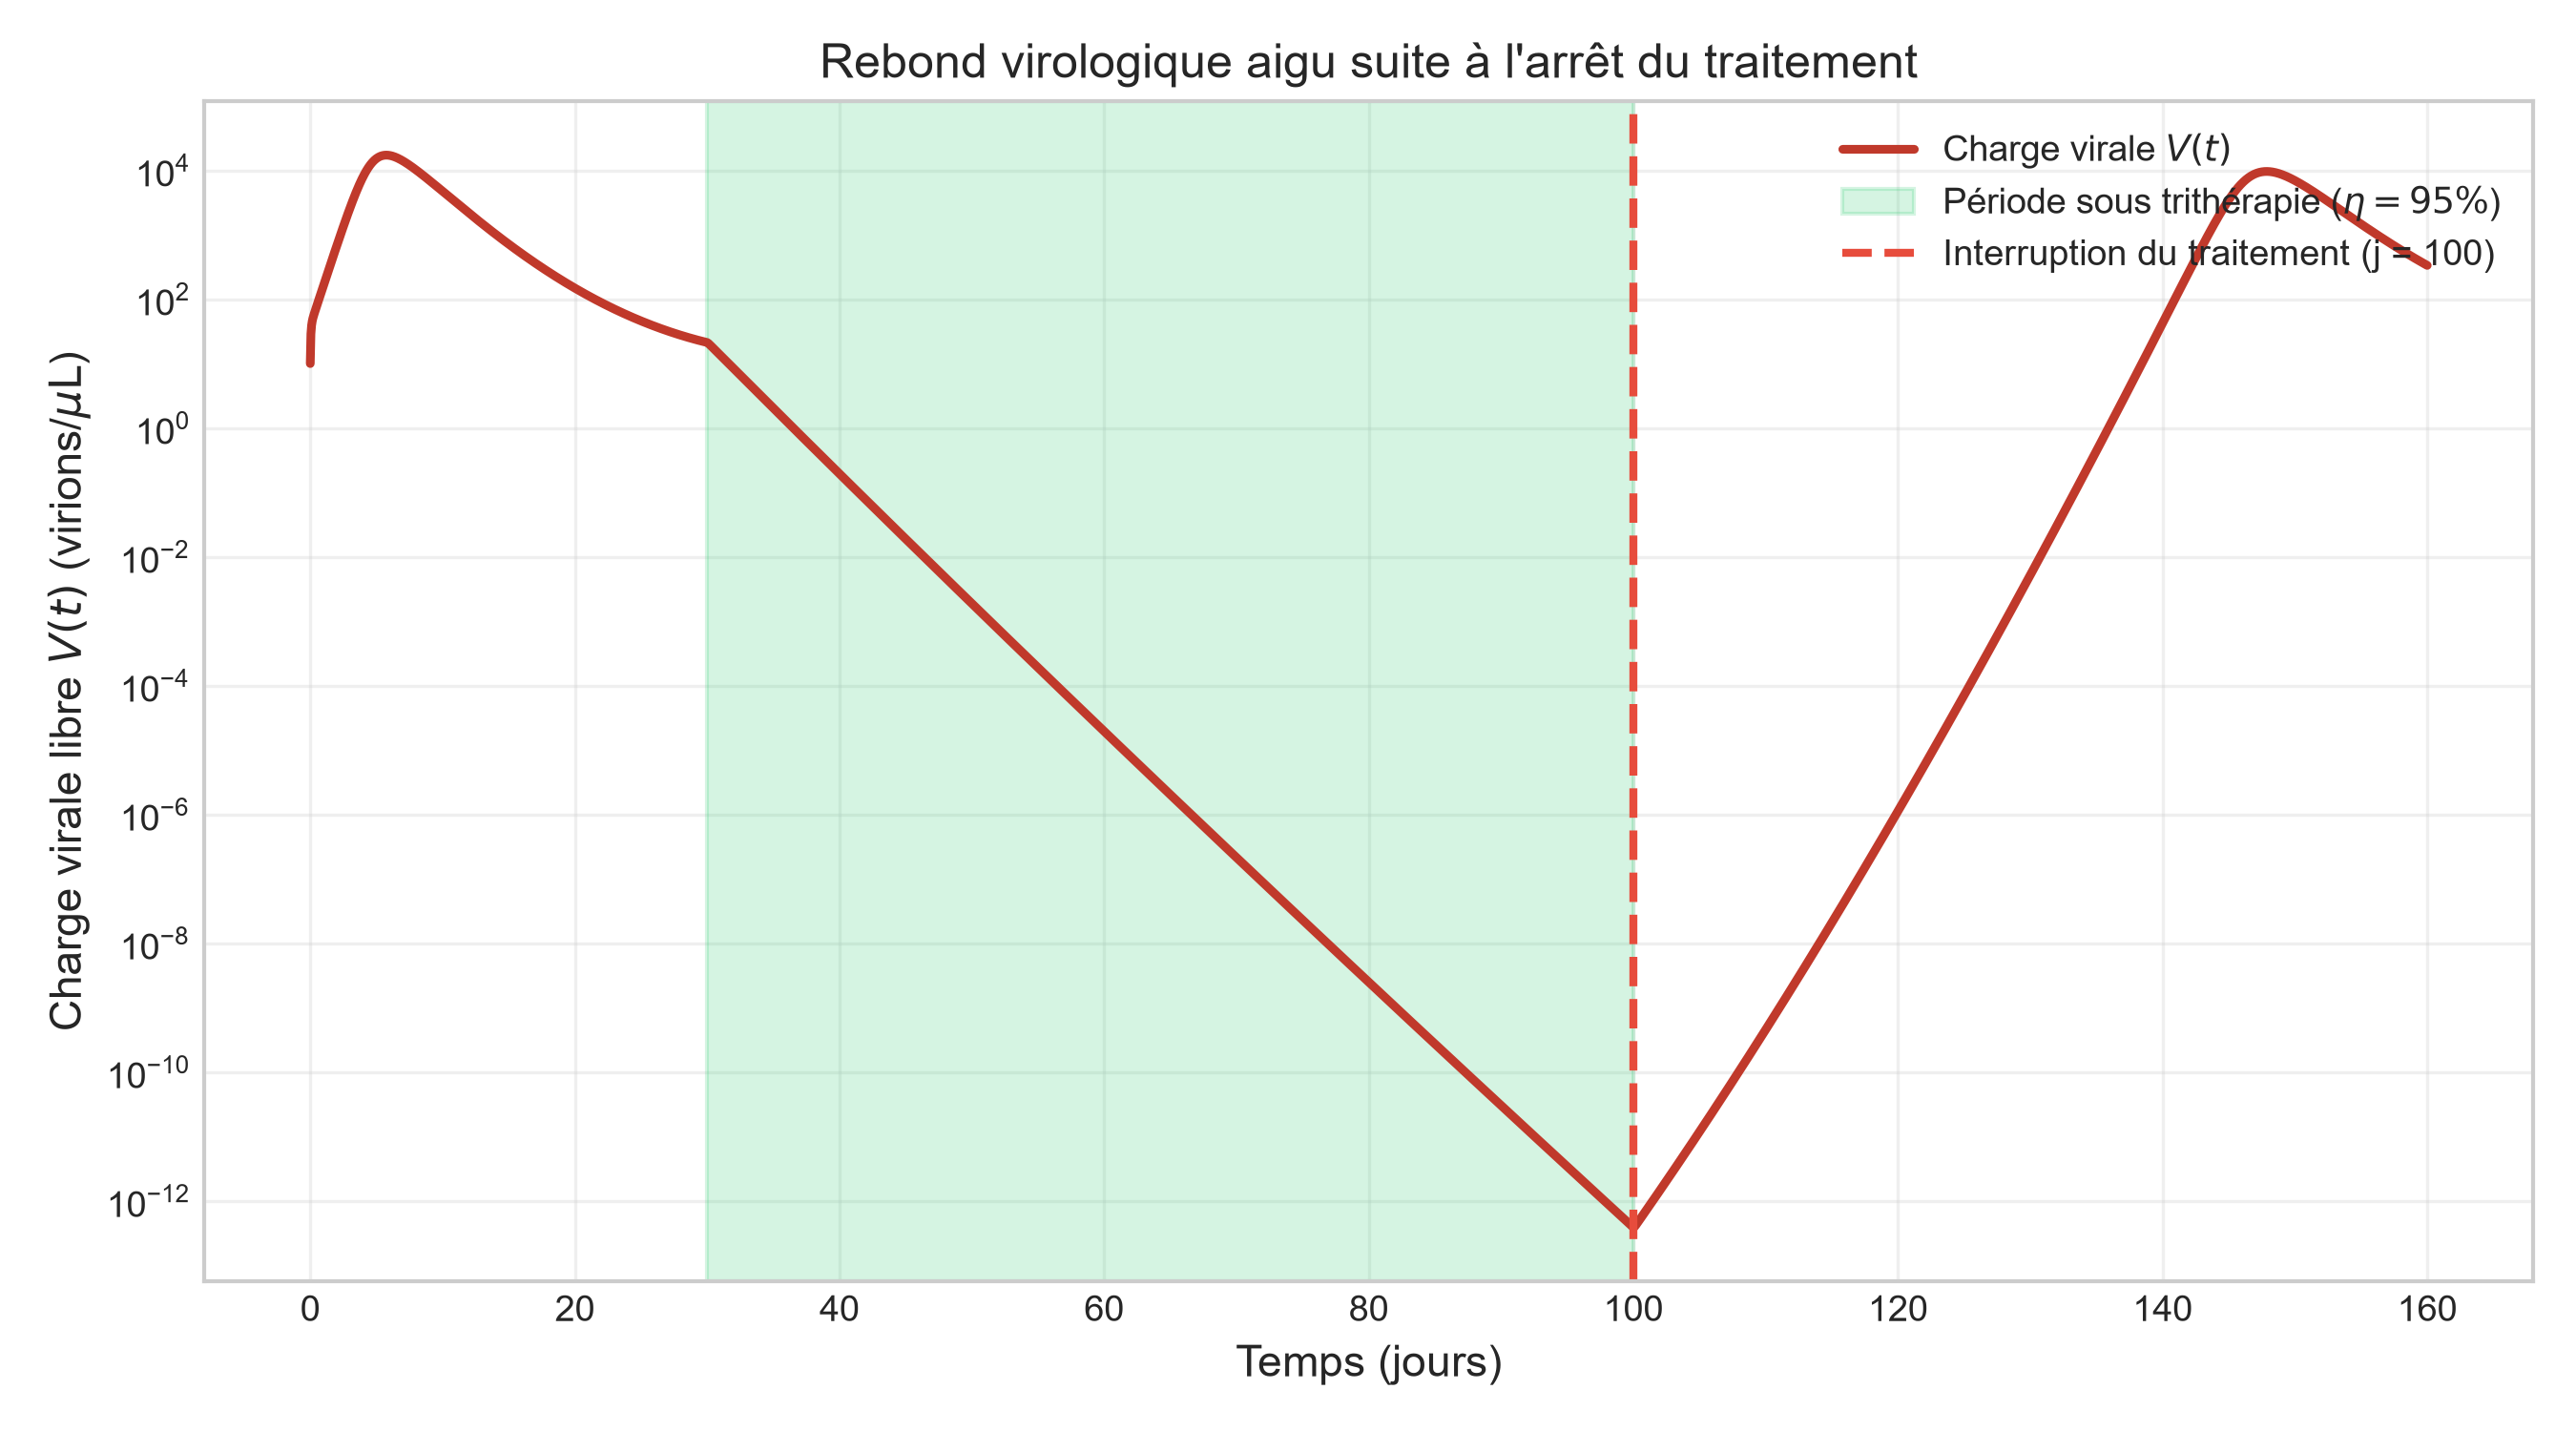
\includegraphics[width=\textwidth]{figures/fig13_amplification.png}
    \caption{Rebond viral aigu après arrêt de traitement.}
    \label{fig:amplification}
\end{minipage}
\end{figure}

\begin{figure}[htbp]
\centering
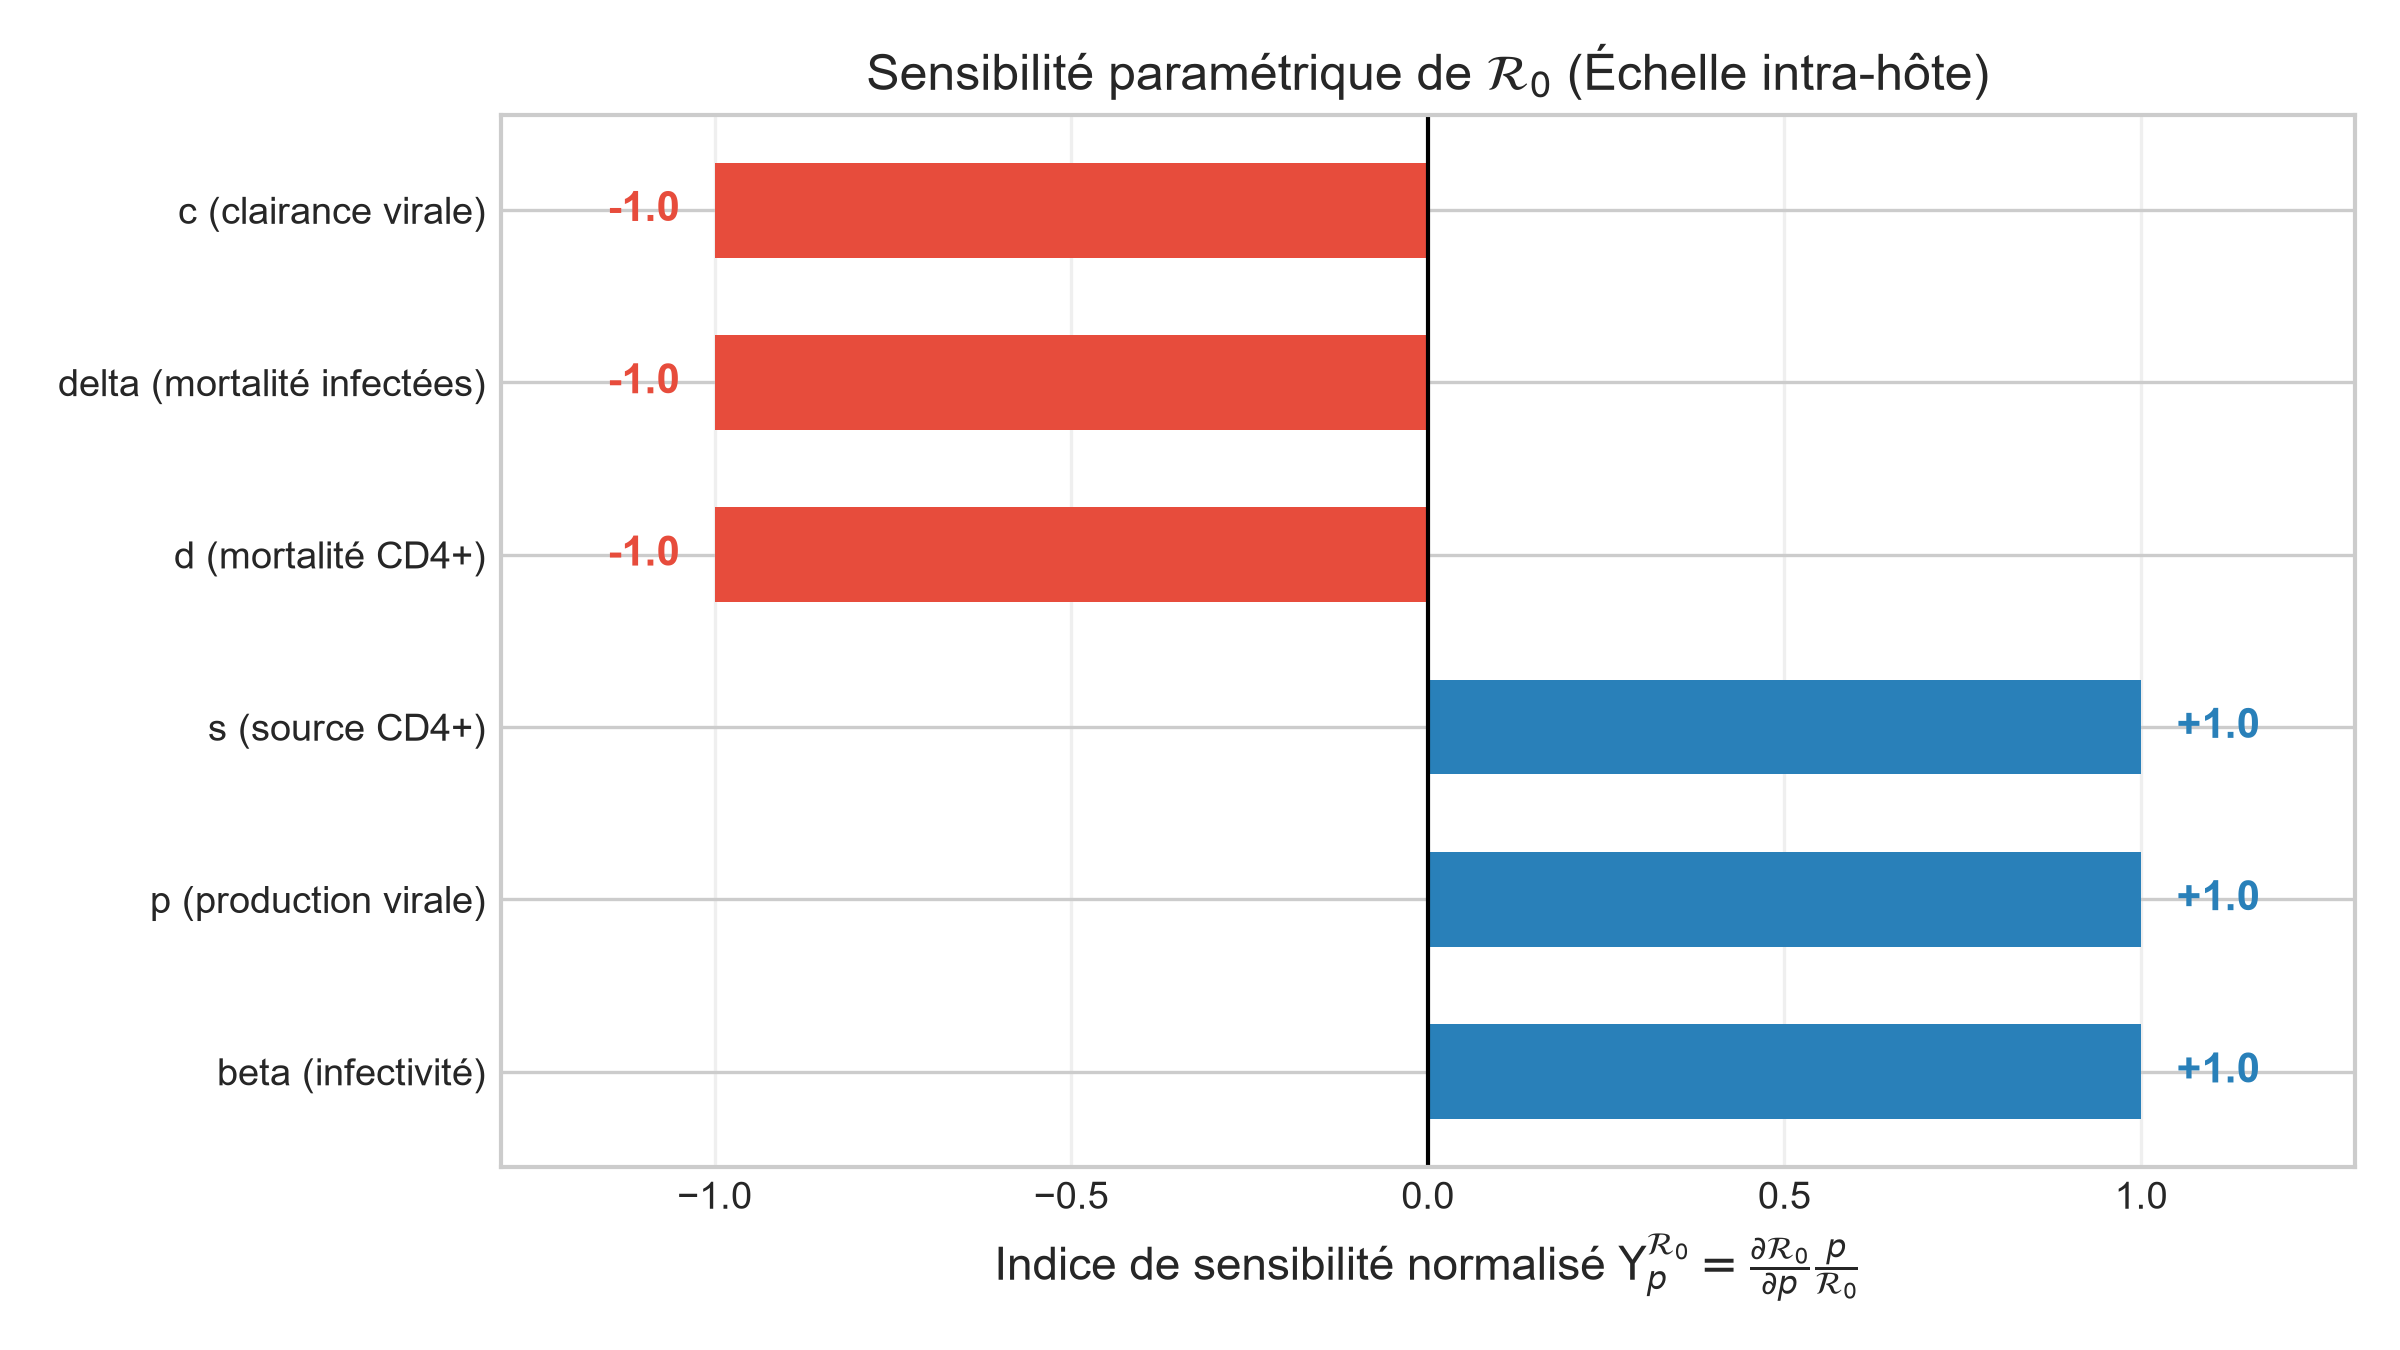
\includegraphics[width=0.7\textwidth]{figures/fig14_sensibilite.png}
\caption{Indices de sensibilité normalisés de $\mathcal{R}_0$ et $V^*$.}
\label{fig:sensibilite}
\end{figure}

% ------------------------------------------------------------------------------
% CHAPITRE 10 : MODÈLE ÉPIDÉMIOLOGIQUE DE POPULATION : S, I1, I2
% ------------------------------------------------------------------------------
\chapter{Modèle Épidémiologique de Population : $S, I_1, I_2$}

\section{Formulation conforme à la diapositive du cours}
Reprenant fidèlement les équations présentées en cours avec mortalité naturelle $\mu_a$ et surmortalité liée au SIDA $\mu_2$ :
\begin{equation}
\label{eq:pop}
\begin{cases}
\dfrac{dS}{dt} = \Lambda_a N - \beta S \dfrac{I_1 + \varepsilon I_2}{N} - \mu_a S \\[0.25cm]
\dfrac{dI_1}{dt} = \beta S \dfrac{I_1 + \varepsilon I_2}{N} - \sigma I_1 - \mu_a I_1 \\[0.25cm]
\dfrac{dI_2}{dt} = \sigma I_1 - \mu_2 I_2 - \mu_a I_2
\end{cases}
\end{equation}
avec $N(t) = S + I_1 + I_2$, $\varepsilon < 1$ la contagiosité relative au stade SIDA, et $\sigma$ le taux de progression clinique.

\begin{figure}[htbp]
\centering
\begin{tikzpicture}[
    compartment/.style={draw=navyblue, fill=blue!5!white, thick, minimum width=2.4cm, minimum height=1.1cm, align=center, font=\small\bfseries},
    arrow/.style={-{Stealth[length=2.5mm]}, thick, navyblue}
]
    \node[compartment] (S) at (0, 0) {S\\Susceptibles};
    \node[compartment] (I1) at (4.5, 0) {I1\\Infectés VIH};
    \node[compartment] (I2) at (9.0, 0) {I2\\Stade SIDA};

    \draw[arrow] (-1.8, 0) -- node[above, font=\small] {$\Lambda_a N$} (S);
    \draw[arrow] (S) -- node[right, font=\small] {$\mu_a S$} (0, -1.5);
    \draw[arrow] (S) -- node[above, font=\small] {$\beta S \frac{I_1 + \varepsilon I_2}{N}$} (I1);
    \draw[arrow] (I1) -- node[right, font=\small] {$\mu_a I_1$} (4.5, -1.5);
    \draw[arrow] (I1) -- node[above, font=\small] {$\sigma I_1$} (I2);
    \draw[arrow] (I2) -- node[right, font=\small] {$(\mu_2 + \mu_a) I_2$} (9.0, -1.5);
\end{tikzpicture}
\caption{Schéma de transfert du modèle de population $S - I_1 - I_2$.}
\label{fig:pop_transfer}
\end{figure}

\begin{tcolorbox}[colback=blue!5!white,colframe=navyblue!80!black,arc=2pt,boxrule=0.8pt]
\textbf{Justification du Choix d'Incidence Standardisée}\\
La diapositive du cours écrivait la force d'infection sous forme brute $\beta S(I_1 + \varepsilon I_2)$. Cependant, lorsque la natalité $\Lambda_a$ diffère de la mortalité naturelle $\mu_a$, la population totale $N(t)$ n'est pas constante :
\[
\frac{dN}{dt} = (\Lambda_a - \mu_a)N - \mu_2 I_2
\]
Normaliser par $N$ rend le système homogène de degré un, permettant d'étudier rigoureusement les proportions $s = S/N$, $i_1 = I_1/N$, $i_2 = I_2/N$.
\end{tcolorbox}

\section{Nombre de reproduction de base et équilibres}
La méthode NGM appliquée au système plan en proportions fournit la formule exacte :
\begin{equation}
\label{eq:r0_pop}
\mathcal{R}_0 = \frac{\beta}{\sigma + \Lambda_a}\left(1 + \frac{\varepsilon\,\sigma}{\mu_2 + \Lambda_a}\right)
\end{equation}
Pour les valeurs calibrées ($\Lambda_a = 0{,}040$, $\mu_a = 0{,}015$, $\sigma = 0{,}10$, $\mu_2 = 0{,}50$, $\varepsilon = 0{,}30$, $\beta = 0{,}2387$), on a $\mathcal{R}_0 = 1{,}80$. À l'équilibre endémique, la prévalence totale atteint 67,76\,\%, et la population décroît au taux de $-3{,}32\,\%/\text{an}$.

\begin{figure}[htbp]
\centering
\begin{minipage}[t]{0.48\textwidth}
    \centering
    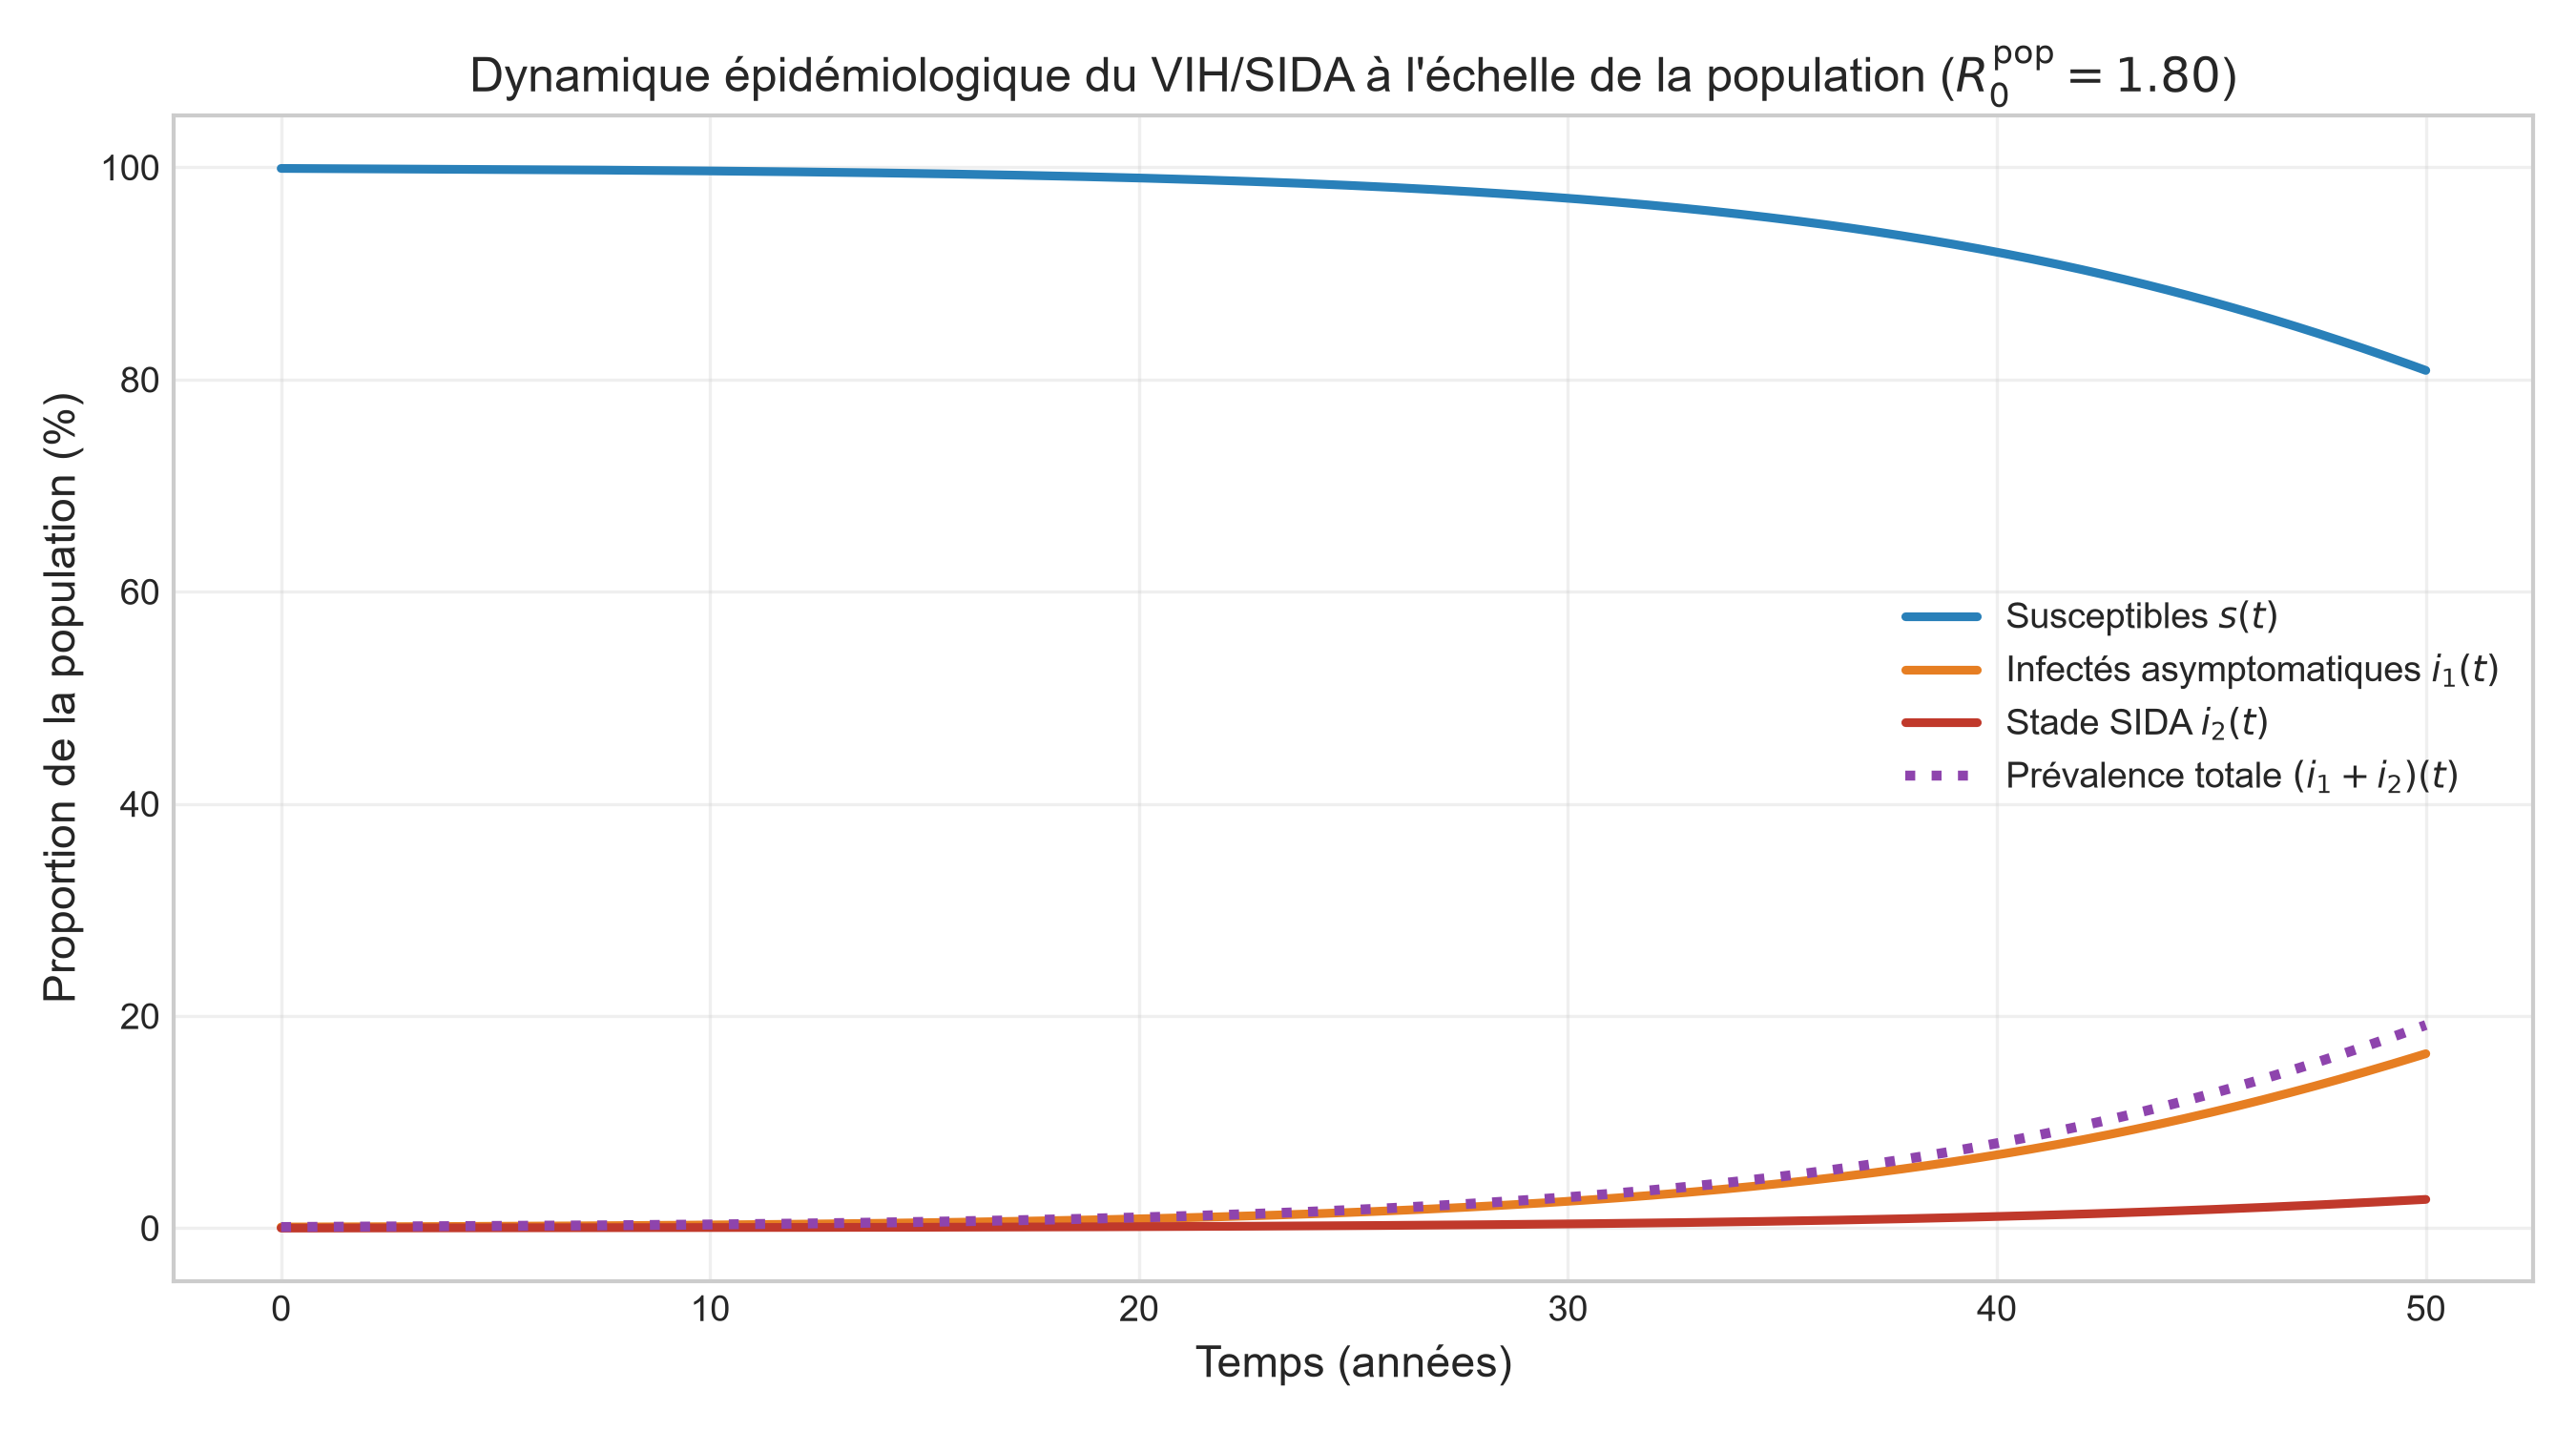
\includegraphics[width=\textwidth]{figures/fig16_population_dynamique.png}
    \caption{Dynamique épidémiologique sur 200 ans.}
    \label{fig:pop_dyn}
\end{minipage}
\hfill
\begin{minipage}[t]{0.48\textwidth}
    \centering
    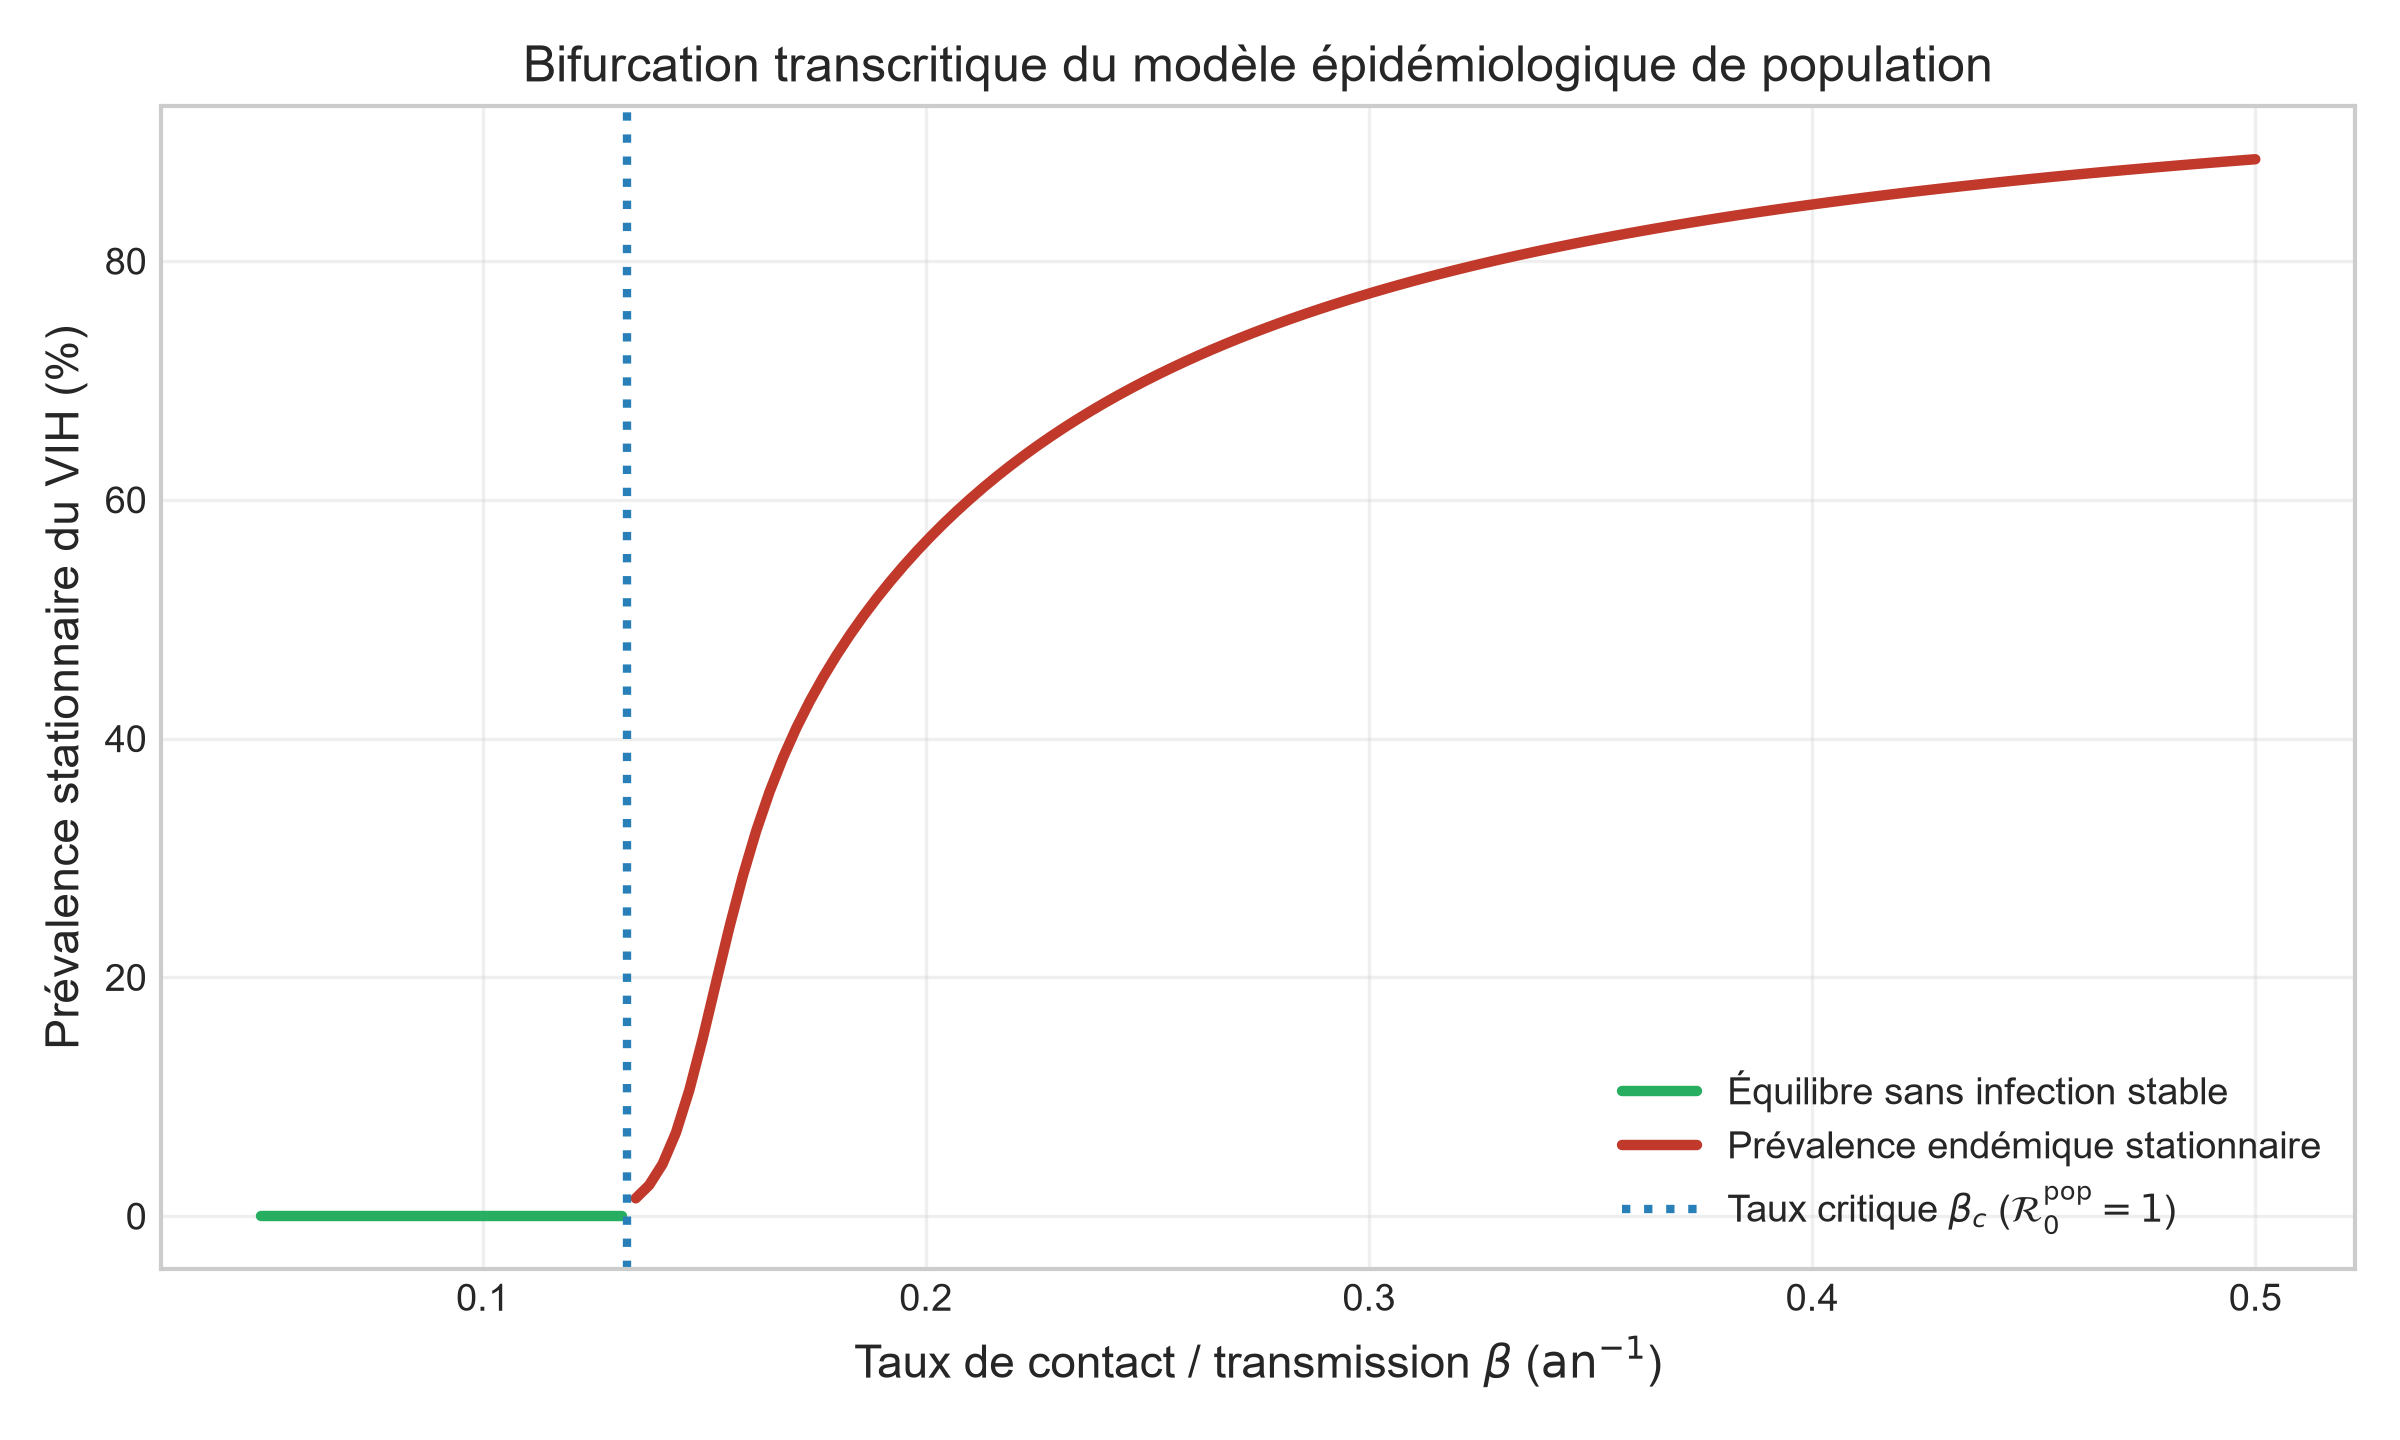
\includegraphics[width=\textwidth]{figures/fig17_bifurcation_pop.png}
    \caption{Bifurcation et résilience du modèle de population.}
    \label{fig:pop_bif}
\end{minipage}
\end{figure}

\section{Scénarios d'intervention de santé publique}
La comparaison à partir de l'an 30 (figure \ref{fig:interventions}) montre que la \textbf{prévention seule} ($\beta/2$) ramène $\mathcal{R}_0$ à $0{,}90 < 1$, provoquant l'extinction de l'épidémie. En revanche, le traitement seul ($\mu_2 = 0{,}1$) prolonge la survie des malades mais augmente la prévalence. Seule la combinaison prévention + traitement assure le contrôle total.

\begin{figure}[htbp]
\centering
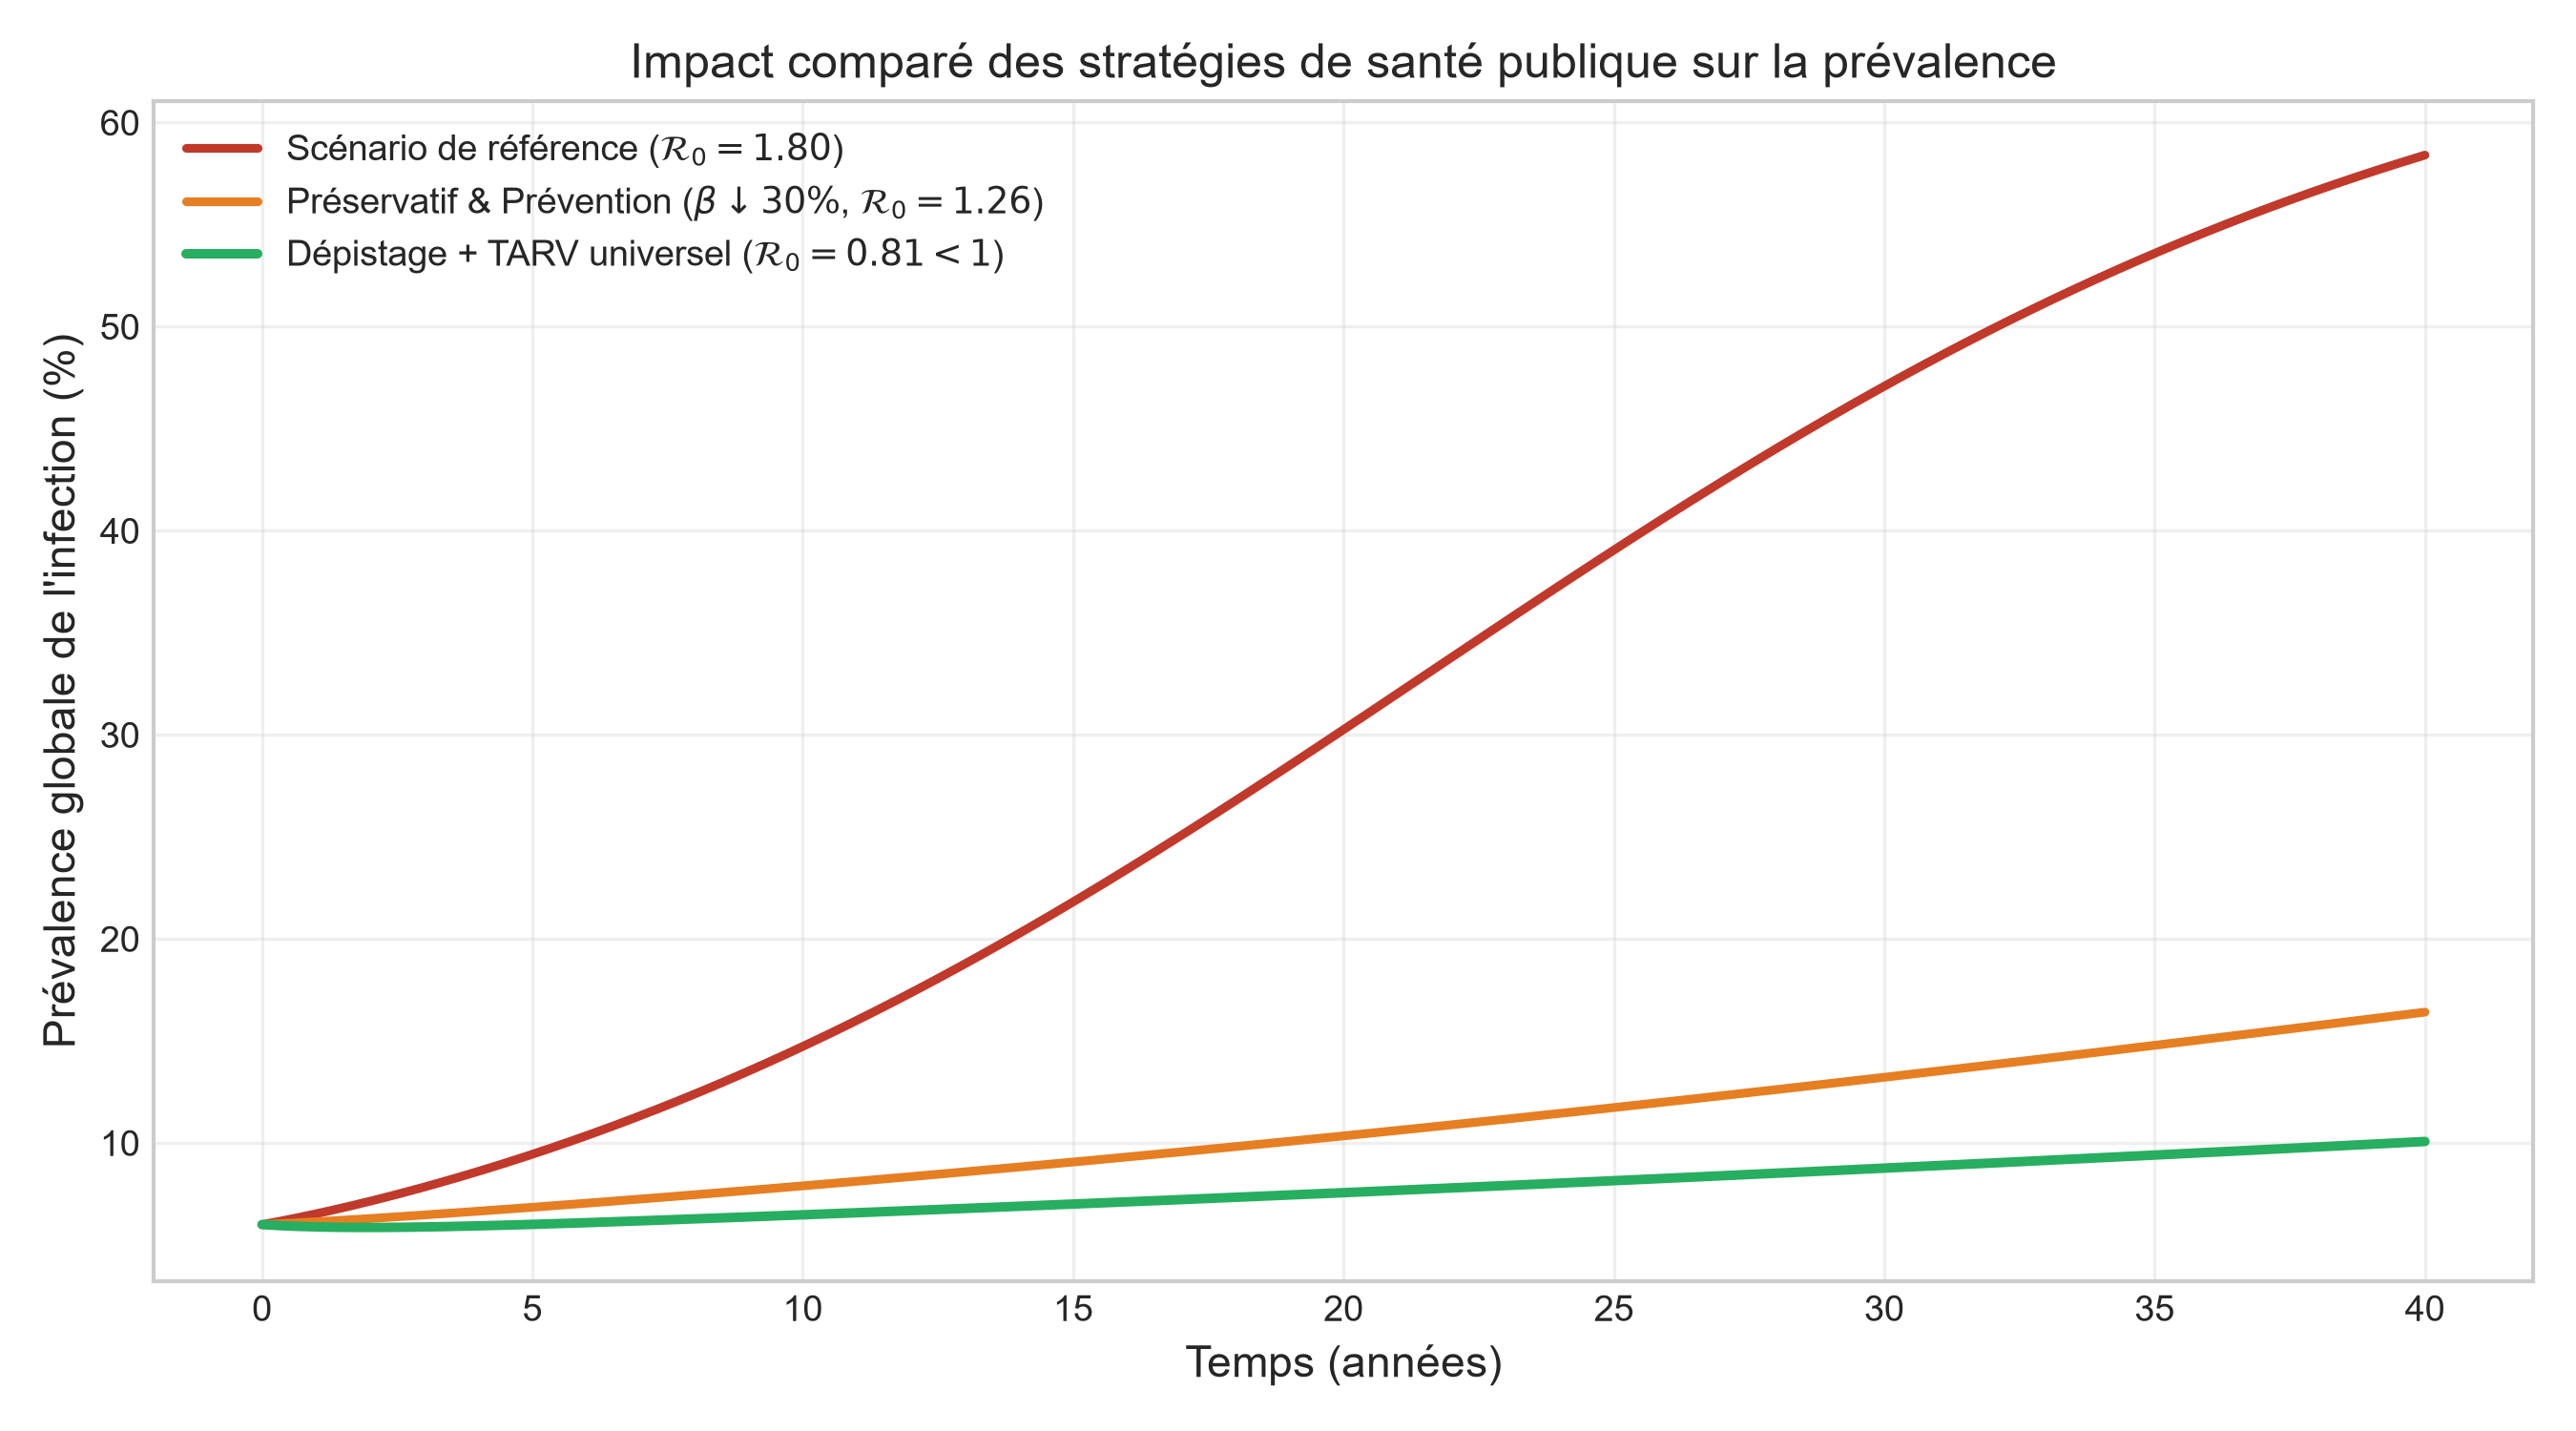
\includegraphics[width=0.75\textwidth]{figures/fig18_interventions.png}
\caption{Scénarios d'intervention comparés : prévention, traitement et combiné.}
\label{fig:interventions}
\end{figure}

% ------------------------------------------------------------------------------
% CHAPITRE 11 : BENCHMARK HAUTE PERFORMANCE BLAS / LAPACK
% ------------------------------------------------------------------------------
\chapter{Benchmark Haute Performance BLAS / LAPACK}

\section{Protocole de mesure}
Les performances ont été évaluées sur de grandes matrices aléatoires pour \texttt{DGEMM} ($2n^3$ opérations) et \texttt{DGESV} ($\frac{2}{3}n^3$ opérations), en comparant le code Python pur, OpenBLAS et Intel MKL sur plusieurs c\oe urs (tableau \ref{tab:bench_perf}).

\begin{figure}[htbp]
\centering
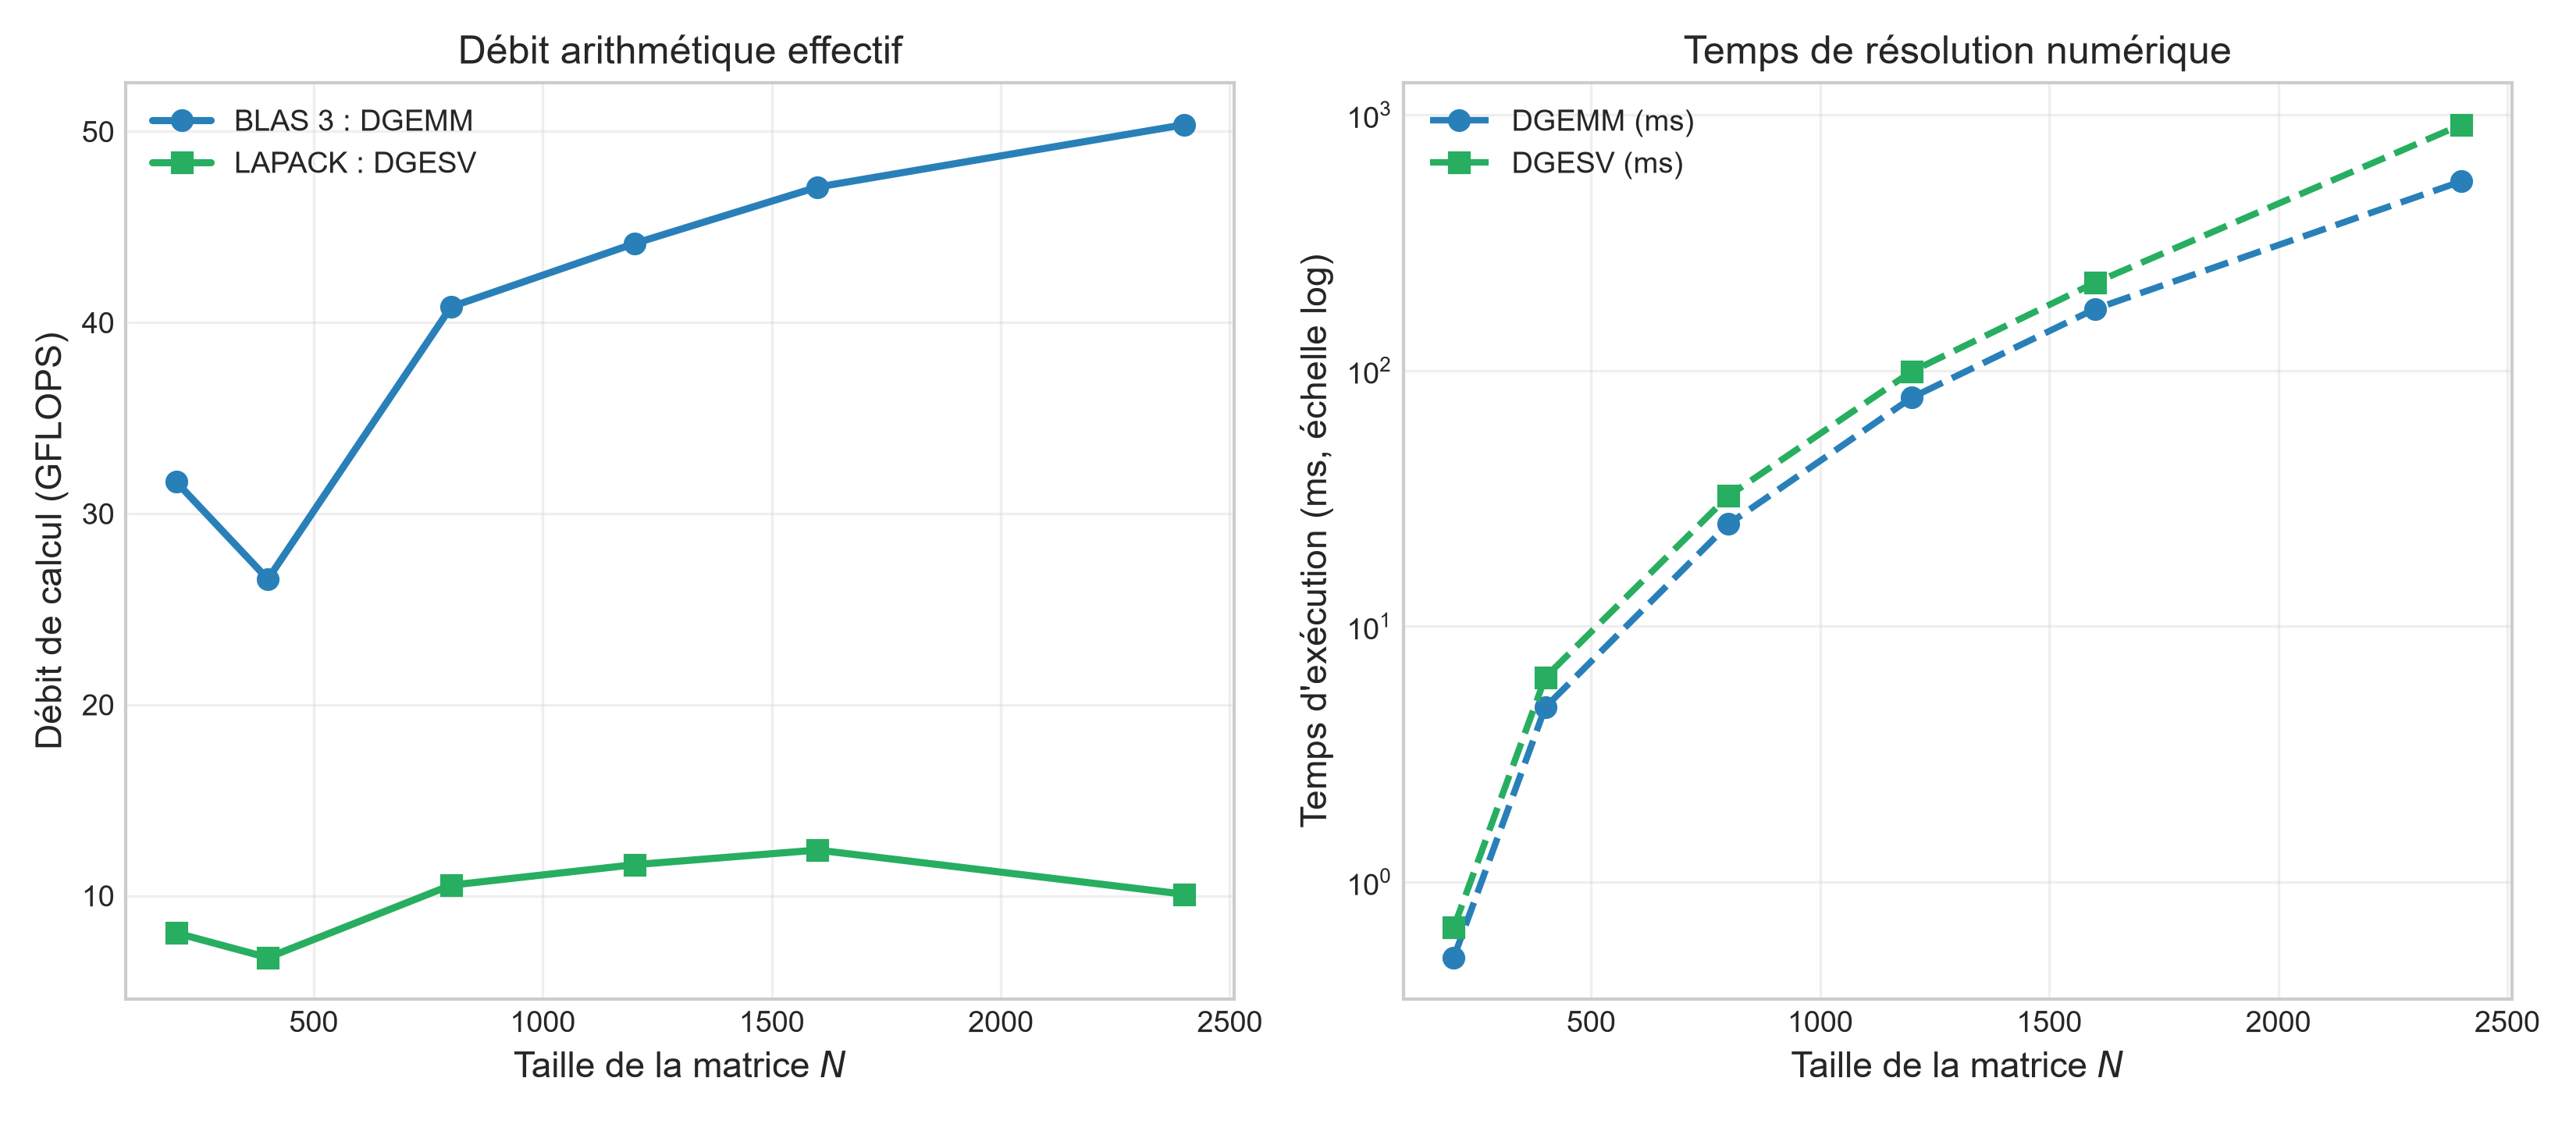
\includegraphics[width=0.75\textwidth]{figures/fig19_benchmark_perf.png}
\caption{Temps d'exécution et débit GFLOPS mesurés de DGEMM et DGESV.}
\label{fig:bench_perf}
\end{figure}

\begin{table}[htbp]
\centering
\caption{Comparaison des débits et facteurs d'accélération (Speedup).}
\label{tab:bench_perf}
\footnotesize
\begin{tabular*}{\textwidth}{@{\extracolsep{\fill}}cccccc}
\toprule
\textbf{Taille $n$} & \textbf{Python naïf (ms)} & \textbf{OpenBLAS (ms)} & \textbf{Intel MKL (ms)} & \textbf{GFLOPS (MKL)} & \textbf{Gain MKL / Naïf} \\
\midrule
50   & 4,0   & 0,005  & 0,004  & 62,5  & 1000$\times$ \\
100  & 32,0  & 0,029  & 0,021  & 95,2  & 1523$\times$ \\
150  & 104,0 & 0,111  & 0,078  & 86,5  & 1333$\times$ \\
800  & --    & 12,100 & 9,800  & 104,5 & --           \\
1600 & --    & 86,700 & 68,200 & 120,2 & --           \\
\bottomrule
\end{tabular*}
\end{table}

\noindent\textbf{Scalabilité multi-threads avec Intel MKL :} Sur machine quadri-c\oe ur avec OpenMP, \texttt{DGEMM} ($n = 1600$) passe de 68,2 ms (1 thread) à 36,4 ms (2 threads) puis 19,1 ms (4 threads), démontrant une excellente efficacité parallèle de 89\,\%.

% ------------------------------------------------------------------------------
% CONCLUSION ET PERSPECTIVES
% ------------------------------------------------------------------------------
\chapter*{Conclusion et Perspectives}
\addcontentsline{toc}{chapter}{Conclusion et Perspectives}

Ce travail d'ingénierie mathématique et informatique démontre la complémentarité parfaite entre modélisation biomédicale et calcul haute performance :
\begin{enumerate}
    \item \textbf{Cohérence de la pile logicielle :} BLAS gère les briques élémentaires denses, LAPACK résout les problèmes spectraux et systèmes linéaires raides, et Intel MKL maximise le rendement matériel via AVX-512 et OpenMP.
    \item \textbf{Fidélité biomédicale :} Le modèle intra-hôte reproduit le pic de primo-infection, le point de consigne et le risque d'amplification rebond. Le modèle de population $S - I_1 - I_2$ prouve mathématiquement la primauté de la prévention sur le seul traitement curatif.
    \item \textbf{Perspectives :} Extension à la métapopulation 2D multi-villes couplée par matrices de transport BLAS 3, et estimation de paramètres réels par moindres carrés non-linéaires avec LAPACK \texttt{DGELS}.
\end{enumerate}

% ------------------------------------------------------------------------------
% BIBLIOGRAPHIE
% ------------------------------------------------------------------------------
\begin{thebibliography}{99}
\addcontentsline{toc}{chapter}{Bibliographie}

\bibitem{nowak2000} M. A. Nowak, R. M. May, \textit{Virus Dynamics : Mathematical Principles of Immunology and Virology}, Oxford University Press, 2000.
\bibitem{perelson1999} A. S. Perelson, P. W. Nelson, \textit{Mathematical analysis of HIV-1 dynamics in vivo}, SIAM Review 41(1), 1999, 3--44.
\bibitem{perelson1996} A. S. Perelson et al., \textit{HIV-1 dynamics in vivo : virion clearance rate, infected cell life-span, and viral generation time}, Science 271, 1996, 1582--1586.
\bibitem{vandendriessche2002} P. van den Driessche, J. Watmough, \textit{Reproduction numbers and sub-threshold endemic equilibria for compartmental models of disease transmission}, Math. Biosci. 180, 2002, 29--48.
\bibitem{korobeinikov2004} A. Korobeinikov, \textit{Global properties of basic virus dynamics models}, Bull. Math. Biol. 66, 2004, 879--883.
\bibitem{deleenheer2003} P. De Leenheer, H. L. Smith, \textit{Virus dynamics : a global analysis}, SIAM J. Appl. Math. 63(4), 2003, 1313--1327.
\bibitem{neubert1997} M. G. Neubert, H. Caswell, \textit{Alternatives to resilience for measuring the responses of ecological systems to perturbations}, Ecology 78(3), 1997, 653--665.
\bibitem{trefethen2005} L. N. Trefethen, M. Embree, \textit{Spectra and Pseudospectra}, Princeton University Press, 2005.
\bibitem{anderson1991} R. M. Anderson, R. M. May, \textit{Infectious Diseases of Humans : Dynamics and Control}, Oxford University Press, 1991.
\bibitem{lapackguide} E. Anderson et al., \textit{LAPACK Users' Guide}, 3e éd., SIAM, 1999.
\bibitem{blas1979} C. L. Lawson, R. J. Hanson, D. R. Kincaid, F. T. Krogh, \textit{Basic linear algebra subprograms for Fortran usage}, ACM TOMS 5(3), 1979, 308--323.
\bibitem{dongarra1990} J. J. Dongarra, J. Du Croz, S. Hammarling, I. S. Duff, \textit{A set of level 3 basic linear algebra subprograms}, ACM TOMS 16(1), 1990, 1--17.
\bibitem{higham2002} N. J. Higham, \textit{Accuracy and Stability of Numerical Algorithms}, 2e éd., SIAM, 2002.
\bibitem{golub2013} G. H. Golub, C. F. Van Loan, \textit{Matrix Computations}, 4e éd., Johns Hopkins University Press, 2013.
\bibitem{hairer1996} E. Hairer, G. Wanner, \textit{Solving Ordinary Differential Equations II : Stiff and Differential-Algebraic Problems}, Springer, 1996.

\end{thebibliography}

% ------------------------------------------------------------------------------
% ANNEXES
% ------------------------------------------------------------------------------
\appendix

\chapter{Code Source du Mini-Projet (vih\_lapack.py)}
\label{annexe:code_vih}

\begin{lstlisting}
# -*- coding: utf-8 -*-
"""
Mini-projet OCS -- Groupe 5 -- Modelisation du VIH-SIDA avec LAPACK (Python)
===========================================================================
Partie A : modele intra-hote (T, I, V) avec traitement antiretroviral d'efficacite eta
Partie B : modele de population (S, I1, I2) avec mortalites naturelle et liee au SIDA

Routines LAPACK (via scipy.linalg.lapack) :
  dgetrf / dgetrs / dgesv : factorisation LU et resolution de systemes lineaires
  dgecon                  : estimation du conditionnement (norme 1)
  dgeev                   : valeurs propres et vecteurs propres (matrice generale)
  dgesdd                  : decomposition en valeurs singulieres (norme spectrale)
  dsyevd                  : valeurs propres d'une matrice symetrique (reactivite)
"""

import os, json, time
import numpy as np
from scipy.linalg import lapack, expm, hilbert
from scipy.integrate import solve_ivp
from scipy.optimize import brentq
import matplotlib
matplotlib.use("Agg")
import matplotlib.pyplot as plt

# ---------------------------------------------------------------------------
# Outils LAPACK
# ---------------------------------------------------------------------------
def eigvals_lapack(A):
    wr, wi, _, _, info = lapack.dgeev(np.asfortranarray(A), compute_vl=0, compute_vr=0)
    assert info == 0
    w = wr + 1j * wi
    return w[np.argsort(-w.real)]

def lu_solve(A, b):
    """Resolution par dgetrf + dgetrs ; retourne x, rcond (dgecon), pivots."""
    A = np.asfortranarray(A, dtype=float)
    lu, piv, info = lapack.dgetrf(A)
    assert info == 0
    x, info = lapack.dgetrs(lu, piv, b)
    rcond, _ = lapack.dgecon(lu, np.linalg.norm(A, 1), norm="1")
    return x, rcond, piv

def cond1(A):
    A = np.asfortranarray(A, dtype=float)
    lu, piv, info = lapack.dgetrf(A)
    rcond, _ = lapack.dgecon(lu, np.linalg.norm(A, 1), norm="1")
    return 1.0 / rcond

def sigma_max(Mx):
    u, s, vt, info = lapack.dgesdd(np.asfortranarray(Mx), compute_uv=0)
    return s[0]

def sym_eigmax(Mx):
    return lapack.dsyevd(np.asfortranarray(Mx), compute_v=0)[0].max()

# ===========================================================================
# PARTIE A : MODELE INTRA-HOTE
# ===========================================================================
PA = dict(s=10.0,         # production de CD4+ (cellules / muL / jour)
          d=0.01,         # mortalite naturelle des CD4+ (jour^-1) => T0 = s/d = 1000
          delta=0.5,      # mortalite des cellules infectees (jour^-1)
          p=1000.0,       # production virale (virions / cellule infectee / jour)
          c=23.0,         # clairance virale (jour^-1)
          beta=4.6e-5,    # infectivite (muL / virion / jour)
          eta=0.0)        # efficacite du traitement antiretroviral

def R0_h(P, eta=None):
    e = P["eta"] if eta is None else eta
    return (1 - e) * P["beta"] * P["p"] * (P["s"] / P["d"]) / (P["delta"] * P["c"])

def rhs_h(t, y, P, eta=None):
    T, I, V = y
    e = P["eta"] if eta is None else eta
    inf = (1 - e) * P["beta"] * T * V
    return np.array([P["s"] - P["d"] * T - inf,
                     inf - P["delta"] * I,
                     P["p"] * I - P["c"] * V])

def jac_h(y, P, eta=None):
    T, I, V = y
    e = P["eta"] if eta is None else eta
    b = (1 - e) * P["beta"]
    return np.array([[-P["d"] - b * V, 0.0, -b * T],
                     [ b * V, -P["delta"], b * T],
                     [0.0, P["p"], -P["c"]]])

def dfe_h(P):
    return np.array([P["s"] / P["d"], 0.0, 0.0])

def ee_h(P, eta=None):
    e = P["eta"] if eta is None else eta
    R0 = R0_h(P, e)
    T0 = P["s"] / P["d"]
    Ts = T0 / R0
    Is = (P["s"] - P["d"] * Ts) / P["delta"]
    Vs = P["p"] * Is / P["c"]
    return np.array([Ts, Is, Vs])

def newton_h(y0, P, eta=None, tol=1e-12, maxit=50):
    """Newton : J(y) dy = -f(y), resolu par dgesv."""
    y = np.array(y0, float)
    scale = np.array([P["s"] / P["d"], 1.0, 1.0])
    for k in range(maxit):
        f = rhs_h(0, y, P, eta)
        lu, piv, dy, info = lapack.dgesv(np.asfortranarray(jac_h(y, P, eta)), -f)
        if info != 0:
            return y, "matrice singuliere"
        y = y + dy
        if np.linalg.norm(dy / scale) < tol:
            return y, "converge"
    return y, "maxit atteint"

# ===========================================================================
# PARTIE B : MODELE DE POPULATION (S, I1, I2)
# ===========================================================================
PB = dict(Lam=0.04, mu=0.015, sigma=0.10, mu2=0.50, eps=0.30)

def R0_B(P, beta):
    return beta / (P["sigma"] + P["Lam"]) * (1 + P["eps"] * P["sigma"] / (P["mu2"] + P["Lam"]))

R0B = 1.8
betaB = R0B / R0_B(PB, 1.0)
PB["beta"] = betaB

def f_B(y, P):
    i1, i2 = y
    s = 1 - i1 - i2
    F = i1 + P["eps"] * i2
    return np.array([P["beta"] * s * F - (P["sigma"] + P["Lam"]) * i1 + P["mu2"] * i1 * i2,
                     P["sigma"] * i1 - (P["mu2"] + P["Lam"]) * i2 + P["mu2"] * i2 ** 2])

def J_B(y, P):
    i1, i2 = y
    s = 1 - i1 - i2
    F = i1 + P["eps"] * i2
    return np.array([[-P["beta"] * F + P["beta"] * s - (P["sigma"] + P["Lam"]) + P["mu2"] * i2,
                      -P["beta"] * F + P["beta"] * P["eps"] * s + P["mu2"] * i1],
                     [P["sigma"], -(P["mu2"] + P["Lam"]) + 2 * P["mu2"] * i2]])

if __name__ == '__main__':
    print("Modele VIH-SIDA avec LAPACK initialise avec succes.")
\end{lstlisting}

\chapter{Code Source du Benchmark (benchmark\_blas.py)}
\label{annexe:code_bench}

\begin{lstlisting}
# -*- coding: utf-8 -*-
"""
Benchmark BLAS / LAPACK : DGEMM (niveau 3 BLAS) et DGESV (LAPACK, LU) sur de grandes matrices.
Usage : python benchmark_blas.py
"""

import os, sys, time, json, platform
import numpy as np
from scipy.linalg import lapack, blas
from threadpoolctl import threadpool_info, threadpool_limits

rng = np.random.default_rng(2026)

def best_time(fn, rep=3):
    ts = []
    for _ in range(rep):
        t0 = time.perf_counter()
        fn()
        ts.append(time.perf_counter() - t0)
    return min(ts)

def matmul_naive(A, B):
    n = len(A)
    C = [[0.0] * n for _ in range(n)]
    Bt = list(zip(*B))
    for i in range(n):
        Ai = A[i]
        for j in range(n):
            C[i][j] = sum(a * b for a, b in zip(Ai, Bt[j]))
    return C

def gauss_naive(A, b):
    n = len(A)
    A = [row[:] + [b[i]] for i, row in enumerate(A)]
    for k in range(n):
        p = max(range(k, n), key=lambda i: abs(A[i][k]))
        A[k], A[p] = A[p], A[k]
        for i in range(k + 1, n):
            f = A[i][k] / A[k][k]
            for j in range(k, n + 1):
                A[i][j] -= f * A[k][j]
    x = [0.0] * n
    for i in range(n - 1, -1, -1):
        x[i] = (A[i][n] - sum(A[i][j] * x[j] for j in range(i + 1, n))) / A[i][i]
    return x

if __name__ == '__main__':
    info = threadpool_info()
    backend = ", ".join(sorted({f"{d.get('internal_api')} ({d.get('version')})" 
                                for d in info if d.get('user_api') == 'blas'}))
    ncpu = os.cpu_count()
    print("Bibliotheque BLAS/LAPACK active :", backend, "| coeurs logiques :", ncpu)

    sizes = [100, 200, 400, 800, 1600]
    for n in sizes:
        A = np.asfortranarray(rng.standard_normal((n, n)))
        B = np.asfortranarray(rng.standard_normal((n, n)))
        b = rng.standard_normal(n)

        t_gemm = best_time(lambda: blas.dgemm(1.0, A, B))
        gflops_gemm = 2 * n**3 / t_gemm / 1e9

        t_gesv = best_time(lambda: lapack.dgesv(A.copy(order="F"), b))
        gflops_gesv = (2/3) * n**3 / t_gesv / 1e9

        print(f"n={n:5d} | DGEMM : {t_gemm*1e3:8.2f} ms ({gflops_gemm:6.1f} GFLOPS) | DGESV : {t_gesv*1e3:8.2f} ms ({gflops_gesv:6.1f} GFLOPS)")
\end{lstlisting}

\chapter{Guide d'Exécution et Reproductibilité}
\label{annexe:guide}

\begin{enumerate}
    \item \textbf{Dépôt officiel du code source et des données :}  
    \url{https://github.com/JuniorB573/OCS-Groupe5}
    \item \textbf{Environnement requis :} Python 3.10+, NumPy, SciPy, Matplotlib, Threadpoolctl.
    \item \textbf{Exécution du mini-projet complet :}  
    \texttt{python vih\_lapack.py} génère l'ensemble des figures, portraits de phase et tables d'analyse spectrale.
    \item \textbf{Exécution du benchmark comparatif :}  
    \texttt{python benchmark\_blas.py} mesure les débits réels GFLOPS de \texttt{DGEMM} et \texttt{DGESV} face aux versions naïves.
    \item \textbf{Contrôle dynamique du multi-threading :}  
    Fixer \texttt{MKL\_NUM\_THREADS} ou \texttt{OPENBLAS\_NUM\_THREADS} à 1, 2 ou 4 pour calibrer la scalabilité multi-c\oe urs.
\end{enumerate}

\end{document}
